\documentclass{article}
 \usepackage[table,xcdraw]{xcolor}
%\documentclass[twocolumn,showpacs,showkeys,preprintnumbers,amsmath,amssymb]{revtex4}
\usepackage[american]{babel}
\usepackage[latin1]{inputenc}
\usepackage{graphicx}
%\usepackage[colorinlistoftodos]{todonotes}
\usepackage{booktabs}
\usepackage{booktabs}
\usepackage{float}
\usepackage{subcaption}
\usepackage{amssymb}
\usepackage{indentfirst}
%\usepackage[numbers]{natbib}
\usepackage[backend=biber]{biblatex}
\addbibresource{poodl-paper.bib}
\begin{document}


\title{Ideologically Motivated Biases in a Multiple Issues Opinion Model}

%\vspace{1cm}

\author{Marcelo V. Maciel \and Andr\'e C. R. Martins\\
  %}
  %\email{amartins@usp.br}
  %\affiliation{%
  NISC - EACH, Universidade de S\~ao Paulo\\
  Av. Arlindo B\'etio, 1000, S\~ao Paulo, 03828-080, Brazil}

%\author{Andr\'e C. R. Martins\\
  %}
 %\email{amartins@usp.br}
 %\affiliation{%
%NISC - EACH, Universidade de S\~ao Paulo\\
%Av. Arlindo B\'etio, 1000, S\~ao Paulo, 03828-080, Brazil}


\date{}


\maketitle
%\vspace{0.3cm}

%\center{\Large\bf Segundo autor}
%\center{\large\bf Afilia��o}


\begin{abstract}
  It has been observed people tend to have opinions that are far more internally
  consistent than it would be reasonable to expect. Here, we study how that
  observation might emerge from changing how agents trust the opinions of their
  peers in a model for opinion dynamics with multiple issues. A previous
  Bayesian inspired opinion model for continuous opinions is extended to include
  multiple issues. In the original model, agents tended to trust less opinions
  that were too different from their own. We investigate the properties of the
  extended model in its natural form. And we also introduce the possibility the
  trust of the agent might depend not only on the specific issue but on the
  average opinions over the many issues. By adopting such a ideological point of
  view, we observe an important decrease in the spread of individual opinions.


  %\keywords{}
  %\pacs{}
\end{abstract}


\section{Introduction}

 % Incluir aqui a parte sobre teoria pol�tica, um par�grafo � suficiente, a princ�pio.

Here, we will present an opinion dynamics model \cite{castellanoetal07,
  galam12a, galametal82, galammoscovici91, sznajd00, deffuantetal00, martins08a}
where the opinions exist over an one-dimensional axis and each agent has a best
estimate on more than one issue over that axis. Describing opinions over a
spatial landscape is an usual way to describe policy alternatives and agents'
preferences. The geometrical properties of the space are usually defined by
mapping from similarity to proximity of the political agents
\cite{downs1957economic, laver2014measuring, tomz2008candidate}. Such a
description can capture the common notion of parties or policies being more ``to
the left'' or ``right''. If they're similar then they're closer
\cite{van2005political, miller2015spatial}. The spatial metaphor is not
restricted to politics it is commonly used in the literature about opinion
dynamics and actually based upon a long research tradition in cognitive science
\cite{aisbett2001general, attneave1950dimensions,gardenfors2004conceptual}.
Major opinions, including political ones, tend to be formed not from only one
issue but from how each person feels about a number of them. Locating someone in
a left versus right or liberal versus conservative axis, therefore, requires
inspecting the opinions of that person in not only one but several issues that
constitute the agent ideological positioning \cite{benoit2006party}.

For many problems, it makes sense to consider different issues as having
components in more than one single dimension \cite{vicenteetal08b}. However, it
is often the case that describing the problem as one-dimensional can be
justified. We can certainly see this as a first approximation along the most
relevant dimension. In that case, the one dimensional case is just a projection
along a direction where variation seems especially important of
higher-dimensional problems. From an application point of view, it is usual to
find discussions to be simplified over only one main disagreement.

One traditional way to model this type of scenario is to use continuous opinions
over a fixed interval, as it is done in the Bounded Confidence (BC) models
\cite{deffuantetal00,hegselmannkrause02}. While discrete models
\cite{galametal82,galammoscovici91,sznajd00} can be very useful at describing
choices, they are not easiest way to represent strength of opinion unless a
continuous variable is associated to the choice \cite{martins08a}. Discrete
models also tend to lack a scale where we can compare opinions and decide which
one is more conservative or more liberal.

On the other hand, continuous models are not particularly well suited for
problems involving discrete decisions. As we will not deal with those kinds of
problems here, they are a natural choice. Indeed, continuous opinions models
have been proposed for several different problems on how opinions spread on a
society \cite{deffuantetal02a,weisbuchetal05}, from questions about the spread
of extremism
\cite{amblarddeffuant04,gargiulomazzoni08a,franksetal08a,alizadeh14a,Albi2016}
to other issues such as how different networks
\cite{Kurmyshev2011,Acemoglu2011,Das2014,Hu2017} or the uncertainty of each
agent \cite{deffuant06} might change how agents influence each other.

Here, we will use a continuous opinion model created by Bayesian-like reasoning
\cite{martins08c}, inspired by the Continuous Opinions and Discrete Actions
(CODA) model \cite{martins08a,martins12b}. That model was shown previously
\cite{martins08c} to provide the same qualitative results as BC models. While a
little less simple, the Bayesian basis makes for a clearer interpretation of the
meaning of the variables. That makes extending the model and interpreting new
results simple. That approach is also consistent with a bounded rationality
variant interpretation of the spatial model of political decision making
\cite{humphreys2010spatial,ostrom1998behavioral}.

Variations of how each agent estimate how trustworthy other agents are will also
be introduced. Here, we use a function of trust $p^*$ that plays a role similar
to the threshold value in BC models. While $p^*$ is not a simple discontinuous
cut-off, it is a function of the distance between the opinions of the agent and
the neighbor. If only one issue is debated, that distance is uniquely defined.
However, if we have multiple issues represented on the same one-dimensional
line, it is not clear which distance we should use. That happens because we have
the opinion of agent $i$ on a specific issue $o_i$ and we can compare it to
$o_j$ to estimate how much $i$ trusts $j$. However, as there are several issues
we could also use the mean opinion of $i$ over all its issues and the same goes
for $j$. Therefore, we will study two additional cases: in the first
alternative, we will change \(p^*\) to \(p^{**}\), determined by the distance
between the neighbor and the agent average opinions. In the second alternative,
we will use a \(p^{***}\) calculated from the opinion of the neighbor and the
average opinion of the agent. The idea here is to make the behavior of our
agents closer to what experiments show about human reasoning. We have observed
that our reasoning about political problems can be better described as
ideologically motivated \cite{jostetal03a,taberlodge06a,Claassen2015a}. Indeed,
our opinions tend to come in blocks even when the issues are logically
independent \cite{jervis76a}. Our reasoning abilities seem to exist more to
defend our main point of views \cite{mercier11a,merciersperber11a} and our
cultural identity \cite{kahanetal11} than to find the best answer. In that
context, evaluating others by how they differ from us as a whole, instead of in
each issue, is a model variation worth exploring.

\section{The Model}
The model is grounded on a Bayesian foundation for opinion dynamics as defended
in \cite{martins12b}. The reason for such a foundation is twofold. First,
opinion dynamics models tend to be created on an ad hoc basis without any clear
connection between them and how each may contribute to the accumulation of
knowledge \cite{flache2017}. The Bayesian approach provides flexible first
principles that allow us to circumvent this problem. Second, even though it is
well documented that people don't faithfully follow the principle of Bayesian
rationality\footnote{For a formal definition of Bayesian rationality see
  \cite[p.104]{gintis2016individuality}.}, many works also indicate that it is a
good \textit{approximation} and that humans are imperfectly bayesian
\cite{tenenbaumetal07,kempetal10a, teglasetal11a, martins05b,
  gintis2016individuality, baker2017rational}. In this framework every agent has
a prior probability distribution about the issue at stake that represents their
knowledge. Agents communicate and the probability that the value stated by a
neighbor $j$, what here we'll call the opinion (\(o\)), is true is the
likelihood that $i$ uses, following an approximate Bayesian rule, to update its
prior probability distribution such that \textbf{posterior opinion distribution}
$\propto$ \textbf{prior} $\times$ \textbf{likelihood}\footnote{For a more
  extensive definition and derivations see \cite{martins12b} and
  \cite{martins2009bayesian} respectively.}.

Here, the population will consist of \(N\) fully connected agents (an agent $i$
can interact with any other agent $j$). Each agent $i$ will have an opinion
$0\leq o_{ik} \leq 1$, where $k=1, \ldots, n$ is a specific issue. We assume
each agent opinion about issue $k$ can represented as a value $o_{ik}$ at the
range of possible values for $o$s. Agents also have an uncertainty $\sigma$
associated to their average estimate $o$. The uncertainty $\sigma$ could be
different for each agent and also updated during the interactions
\cite{martins08c}. For the sake of simplicity, however, we will assume the
uncertainty $\sigma_i =\sigma$ is identical for (almost) all agents and it does
not change. The set of opinions for each agent on all possible issues will
define its ideological profile \(I_i = ( (o_{i 1}, \sigma), \ldots, (o_{i n},
\sigma) ) \) , where \(n\) is the number of issues, \(o\) is the opinion about
the issue and \(\sigma\) is the global uncertainty~\cite{martins2009bayesian}.
The arithmetic mean $x_i$ of agent $i$ opinions in each issue will be called
here the ideal point for each agent, that is, it defines the agent ideological
position at the dimension of interest \cite{armstrong2014analyzing}. Obviously
\( x_i = \frac{1}{n} \sum_{k=1}^{n} o_{ik} \).

In order to have agents with initial ideal points well distributed over the
possible range, the initial valued for each \(o_{ik}\) was randomly drawn
using a Beta \(Be(\alpha, \beta)\) with random parameters $\alpha_i$ and
$\beta_i$. Those parameters were drawn for each agent $i$ from the ranges \( (
\alpha \in [1.1, 100], \beta \in [1.1, 100] ) \) by dividing those ranges by
\(N\) equally spaced values and then assigning them to each agent after mixing
the values as in a Latin hypercube sampling~\cite{mckay2000comparison}. That is done to
allow agents with a diverse value of initial ideal points and, at the same time,
to keep the initial \(o_{ik}\)s of each agent $i$ correlated.


While we could have \(\sigma\) as a measurement of each agent uncertainty and
have it evolve with time, here we will keep it as a fixed parameter of the
model. However, a proportion \textit{p$\_$intran} of agents will be stubborn
about one single issue $k$, so that \(\sigma_{ik} \approxeq 0\) (implemented as
1e-20). That behavior is kept constant as the simulation unfolds, that is
$\sigma_{ik}$ is also not updated by the model. A proportion of agents who are
stubborn is introduced here so we can check if inflexible
\cite{galam05b,deffuant2002can,martinsgalam13a} have a significant impact on the
outcomes of the model.


%For its part, \(\sigma\) is a parameter of the model, not the agents. However, a
%proportion \textit{p$\_$intran} of the agents will have an unique \(\sigma_{i,k}
%= 1e-20\). This is done so that wesuch as “how much each agent trusts another agent should be a function can control for the impact of inflexible
%agents on the model dynamics \cite{galam05b,deffuant2002can,martinsgalam13a}.

%How many agents are intransigent is also a parameter (coded as
%\textit{p$\_$intran} ), and such \(\sigma\) is established at the initial
%condition by sampling the issue index from the \(I_i\)'s length. This means that
%we've opted for an implementation in which agents are intransigents in a
%\textit{single} issue.

In each iteration of the simulation, two procedures are applied: the
opinion update through social influence, and a random opinion update (noise). In
the social influence procedure we draw two agents, \(i\) and \(j\), from the
population, where \(i\) will observe \(j\) opinion about a randomly drawn issue \(k
\in (1 , \ldots, n)\). %That way, we have the corresponding pairs (\(o_{i,k},
%o_{j,k}\)) and (\(\sigma_{i,k}, \sigma_{j,k}\)).
Agent \(i\) updates its opinion (\(o_{ik}\)) following an approximate Bayesian
rule. That rule is obtained by assuming each agent has a Normal prior
\(f_i(\theta) = \frac{1}{\sqrt{2 \pi} \sigma_i} e^{- \frac{(\theta - o_i )^2}{2
    \sigma_i}} \) compatible with its parameters $o_{i}$ and $\sigma_{i}$, where
the index related to the issue $k$ was omitted for the sake of simplifying the
equation. The agents also assume a mixture likelihood where there is an initial
chance \(p\), updated to \(p^*\) that the agent \(j\) has information and a
chance \(1-p\) it knows nothing and its opinion is just a random non-informative
draw. That is, the likelhood is given by \( f(o_j|\theta) = p
N(\theta,\sigma_j^2) + (1-p)U(0,1) \). While a full Bayesian treatment would
produce a posterior distribution that is a mixture of two normals, here we will
assume each agent only updates its expected value and it does not carry the full
posterior information to the next iteration. That leads to the following update
rule for the expected value $o_{i,k}$ \cite{martins2009bayesian}:


  \begin{equation}\label{eq:oupdate}
    o_{ik}(t+1) =
    p^{*}
    \frac{o_{ik}(t) + o_{jk}(t) }{2}
    +
    (1 - p^{*})
    o_{ik}(t),
  \end{equation}
where  $p^{*}$ is given by
  \begin{equation}\label{eq:pstar}
   p^{*}
    =
  \frac{
      p \frac{1}{\sqrt{2 \pi} \sigma_i}
      e^{- \frac{ (\Delta_{ij})^2}{2 \sigma_i^2}}
    }{
      p
      \frac{1}{\sqrt{2 \pi} \sigma_i}
    e^{- \frac{ ( \Delta_{ij})^2}{2 \sigma_i^2}}
    +
    (1 - p)
  }.
\end{equation}

Here \(\Delta_{ij} = o_{ik} (t) - o_{jk} (t)\) is the distance between the
opinions on the $k$ issue. As $\Delta_{ij}$ increases, it is easy to see that
Equation \ref{eq:pstar} causes $p^{*}$ to tend to zero. Given this relationship,
$\Delta_{ij}$ plays a similar role to the threshold parameter in the Bounded
Confidence models by making distant opinions less influential. And, as that
happens, the weights in average update Equation~\ref{eq:oupdate} change so that
the previous value $ o_{i,k}(t)$ remains almost unchanged.

The threshold role of $\Delta_{ij}$ suggests we might change its definition to
check how it might better reflect the actual behavior of humans. In particular,
people tend to trust better those who have a similar ideology. That means trust
might not depend on the specific issue alone, but on the average over all
issues. While that is not the model we obtain from applying Bayes rule, such a
change makes sense as an attempt to have a better model. In order to check that
possibility we will also implement two other cases by changing the way
$\Delta_{ij}$ is calculated. In the first variation, $p^*$ will be substituted
by \(p^{**}\), where \(p^{**}\) means \(\Delta_{ij} = x_i(t) - x_j(t) \), that
is, agent $i$ will observe the average ideological position of $j$ in order to
estimate its trust. That assumed $i$ has more information than only the value
$o_{jk}(t)$. To check what happens when only $o_{jk}(t)$ can be observed by
agent $i$, we will introduce a second variant case where $i$ compares
$o_{jk}(t)$ to its own average. That is, \(\Delta_{ij} = x_{i}(t) - o_{jk}(t)\)
and we represent that case by \(p^{***}\).

In order to better understand the model dynamics we also introduce noise as the
second procedure. At each iteration, another agent \(i\) is randomly chosen and
its opinion changed due to random noise. That is, $i$ opinion becomes \(
o_{ik}(t+1) = o_{ik}(t) + r \) where \(r\) is drawn from a Normal distribution
with mean 0 and standard deviation \(\rho\). If agent \(i\) is intransigent in
issue \(k\) it won't its \(o_{ik}\) opinion when chosen by the noise algorithm.
Moreover, if \(o_{ik}(t) + r > 1\) then \( o_{ik}(t+1) = 1\). Likewise, if
\(o_{ik}(t) + r < 0 \) then \( o_{ik}(t+1) = 0\). Noise is introduced here as a
way of accounting for the effect of factors not related to the modeled social
influence \cite{flache2017} and it is interesting to verify if small noises can
lead to drastic changes in systemic properties \cite{macy2015signal}.

  \section{Model Results}

  To better understand the model behavior, we ran simulations using as range for
  the parameters the values:

  \begin{table}[H]
    \centering
\begin{tabular}{@{}|l|l|l|l|l|l|@{}}
\toprule
\rowcolor[HTML]{EFEFEF}
$\sigma$ & $n$ & $p$ & $p\_intran$ & $N$ & $\rho$ \\ \midrule
$[0.01, 0.5]$ & $[1, 10]$  & $[0.1, 0.99]$ & $[0.0, 0.1]$ & $[500, 5000]$ & $(0.0, 0.1]$ \\ \bottomrule
\end{tabular}
\caption{Parameters' Bounds}
\end{table}

The parameter space was explored by two sweeps of its parameters: one sampling
of 70,000 quasi-random low-discrepancy sequence draws on all parameters
\cite{saltelli2008global, saltelli2000sensitivity}, that generate evenly spaced
points, and another of 60,000 keeping \(N=500\) so that we can compare different
realizations. An interesting question in any opinion dynamics model is if agents
can reach consensus, if they diverge, or something between those two states.
That can be observed by comparing the initial mean and standard deviation of
each agent's opinions. Figure \ref{fig:std} shows histograms for those variables
at the initial condition and also for the final opinions corresponding to the
(\(p^{*}, p^{**}, p^{***}\)) cases. The upper graphic shows the distribution of
the mean opinions $x_i$, and the lower one the distribution of the standard
deviation of the opinions of each agent $s_i^2== \frac{1}{n} \sum_{k=1}^{n}
(o_{ik}-x_i)^2$. That is, for each case we sampled 60,000 parameterizations
guaranteeing that we're filling evenly the space of parameters' possible values.
Then we collected the mean and standard deviation of the opinions \textit{of
  each agent} for each parameterization both at the initial and final
conditions. Figure \ref{fig:std} then gives a general view of the model behavior
as we are plotting many different combinations of parameters' values.

\begin{figure}[H]
  \centering \captionsetup{justification=centering,margin=2cm}

  \begin{subfigure}[h]{0.85\textwidth}
    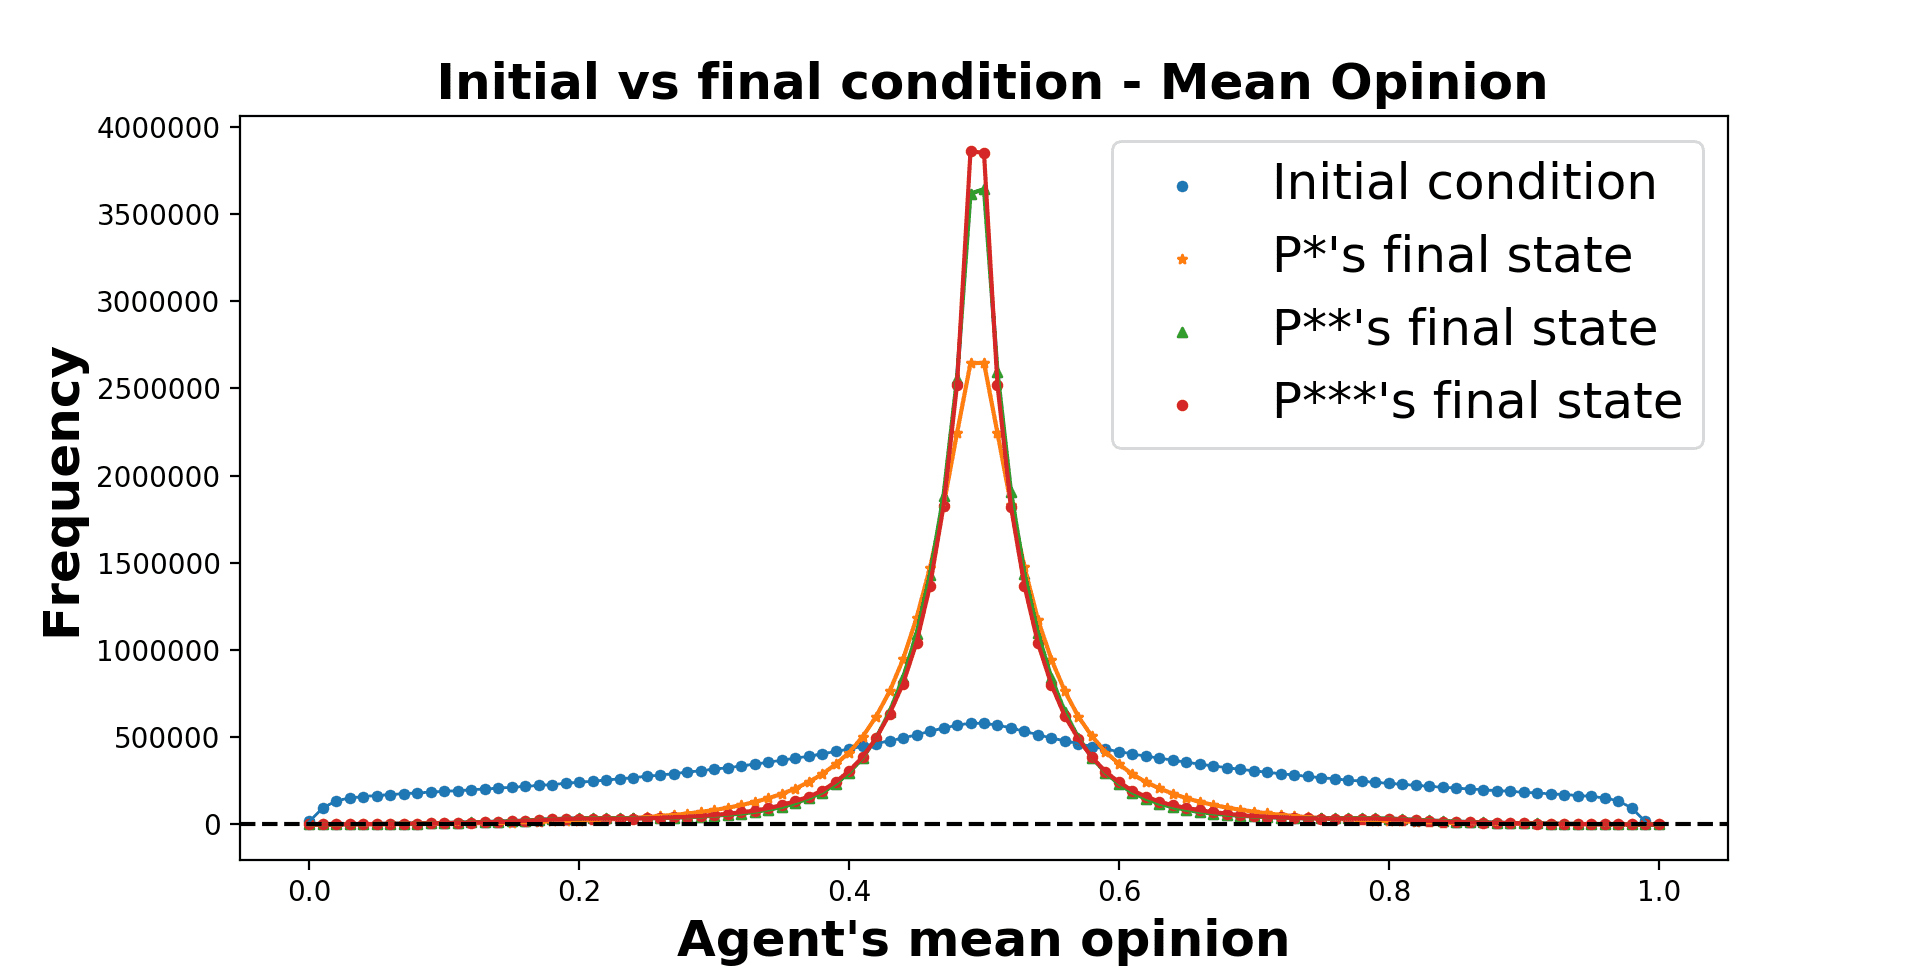
\includegraphics[width=\textwidth]{img/mean_hist.png}
    \caption{Initial x Final state: \\ Distribution of mean opinions}
  \end{subfigure}
  \begin{subfigure}[b]{0.85\textwidth}
    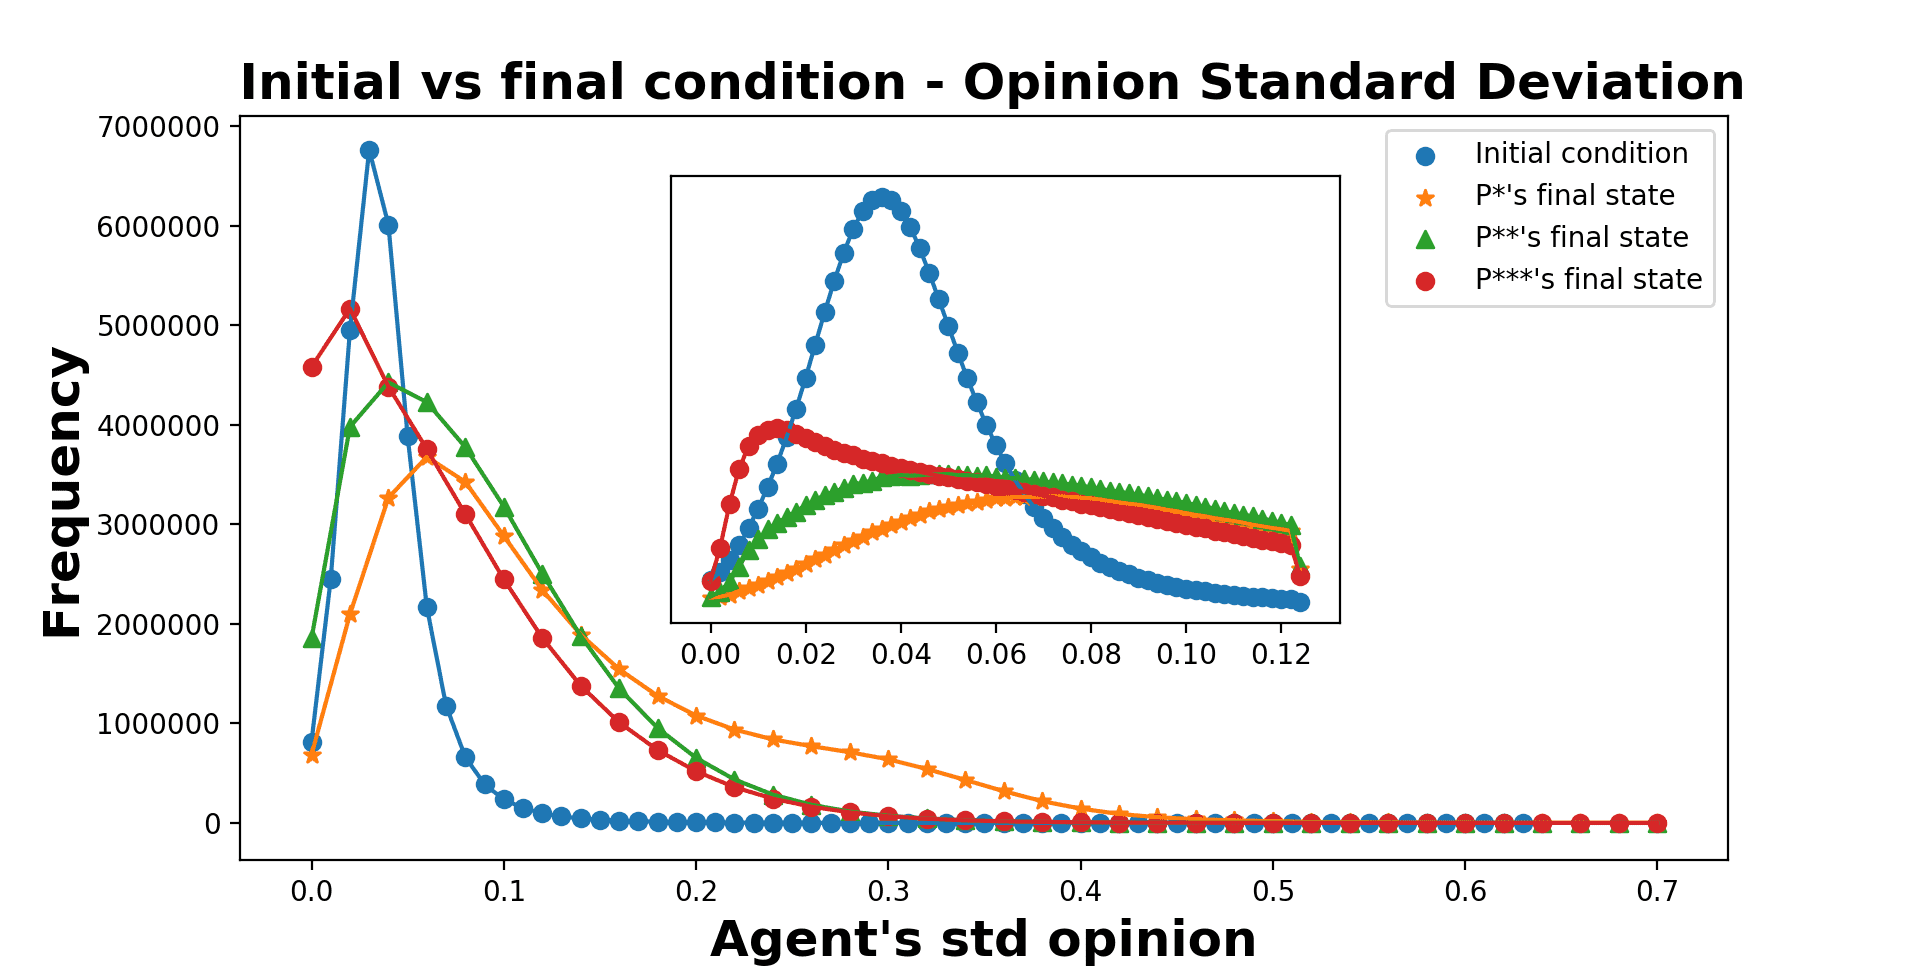
\includegraphics[width=\textwidth]{img/std_hist2.png}
    \caption{Initial x Final state: \\ Distribution of the standard deviations of opinions}
  \end{subfigure}
  \caption{Difference between initial and final opinion distributions for 60.000
    parameterizations. In all cases, \(N = 500\).}
  \label{fig:std}
\end{figure}

The histograms show that, in general, opinions have a tendency to move towards
the middle value. This seems to suggest most parameter values lead to consensus
or near it. However, consensus is not always achieved, as shown by the tails of
the mean distribution at Figure \ref{fig:std}, even if the final distribution
shows that extreme opinions become less common. And we can also observe in the
distribution of standard deviations $s_i$ that the opinions of each agent on
each issue tend to become more diverse, as, for most cases, $s_i$ seems to
increase from its initial values. The only exception is the $p^{***}$ scenario.
There, we still see an increase in the frequency of large values of $s_i$. But
there are also many cases where there is a strong tendency for $s_i$ to become
smaller. Or, in other words, in several scenarios, the agents opinions on the
issues tended to gather much closer to their own mean opinions $x_i$ as a
consequence of the dynamics.

The cases where the average opinions remain a little spread, while rare,
correspond to scenarios where bi-partisanship survives, with agents opinions
surviving at both extreme positions. This suggests that, in general, the model
can be described as one with similarity biased influence \cite{flache2017}. This
tendency to consensus seems to be a little weaker at the \(p^*\) case when
compared to the two other cases, $p^{**}$ and $p^{***}$.


Figure \ref{fig:std} (b) also shows that in all cases (\(p^{*}, p^{**},
p^{***}\)) the standard deviation of the opinions distribution becomes more
spread. While there are situations where $s_i$ tends to become smaller,
signaling the agent opinions become closer to its mean, the reverse also
happens. The tails for larger values of $s_i$ show that the intercation with
other agents quite often led to a more diverse set of opinions over the
different issues. As a matter of fact, except for the $p^{***}$ scenarios, a
larger internal spread than in the initial conditions seem to be the usual
result. For $p^{***}$, while we also observe that strenghtening of the spread
for many parameter values, we also see that an increase in cases with small
$s_i$. That is, the dynamics can lead to stronger internal consistency.

The distributions for the mean and standard deviation might look contradictory
at a first glance. But they are information about different quantities. A
tendency of the $x_i$ towards central value while $s_i$ increases is simple to
understand. It just shows that, while opinions on different issues might be
spreading more, including towards more extreme values, the mean of every issue
opinion of the agents show a clear central tendency. That the mean would have a
central tendency should not be seen as a surprise. But that does not necessarily
correspond to what happens to the agents  opinions on specific issues $o_{ik}$.

    \begin{figure}[H]
  \centering
    \begin{subfigure}[b]{0.49\textwidth}
      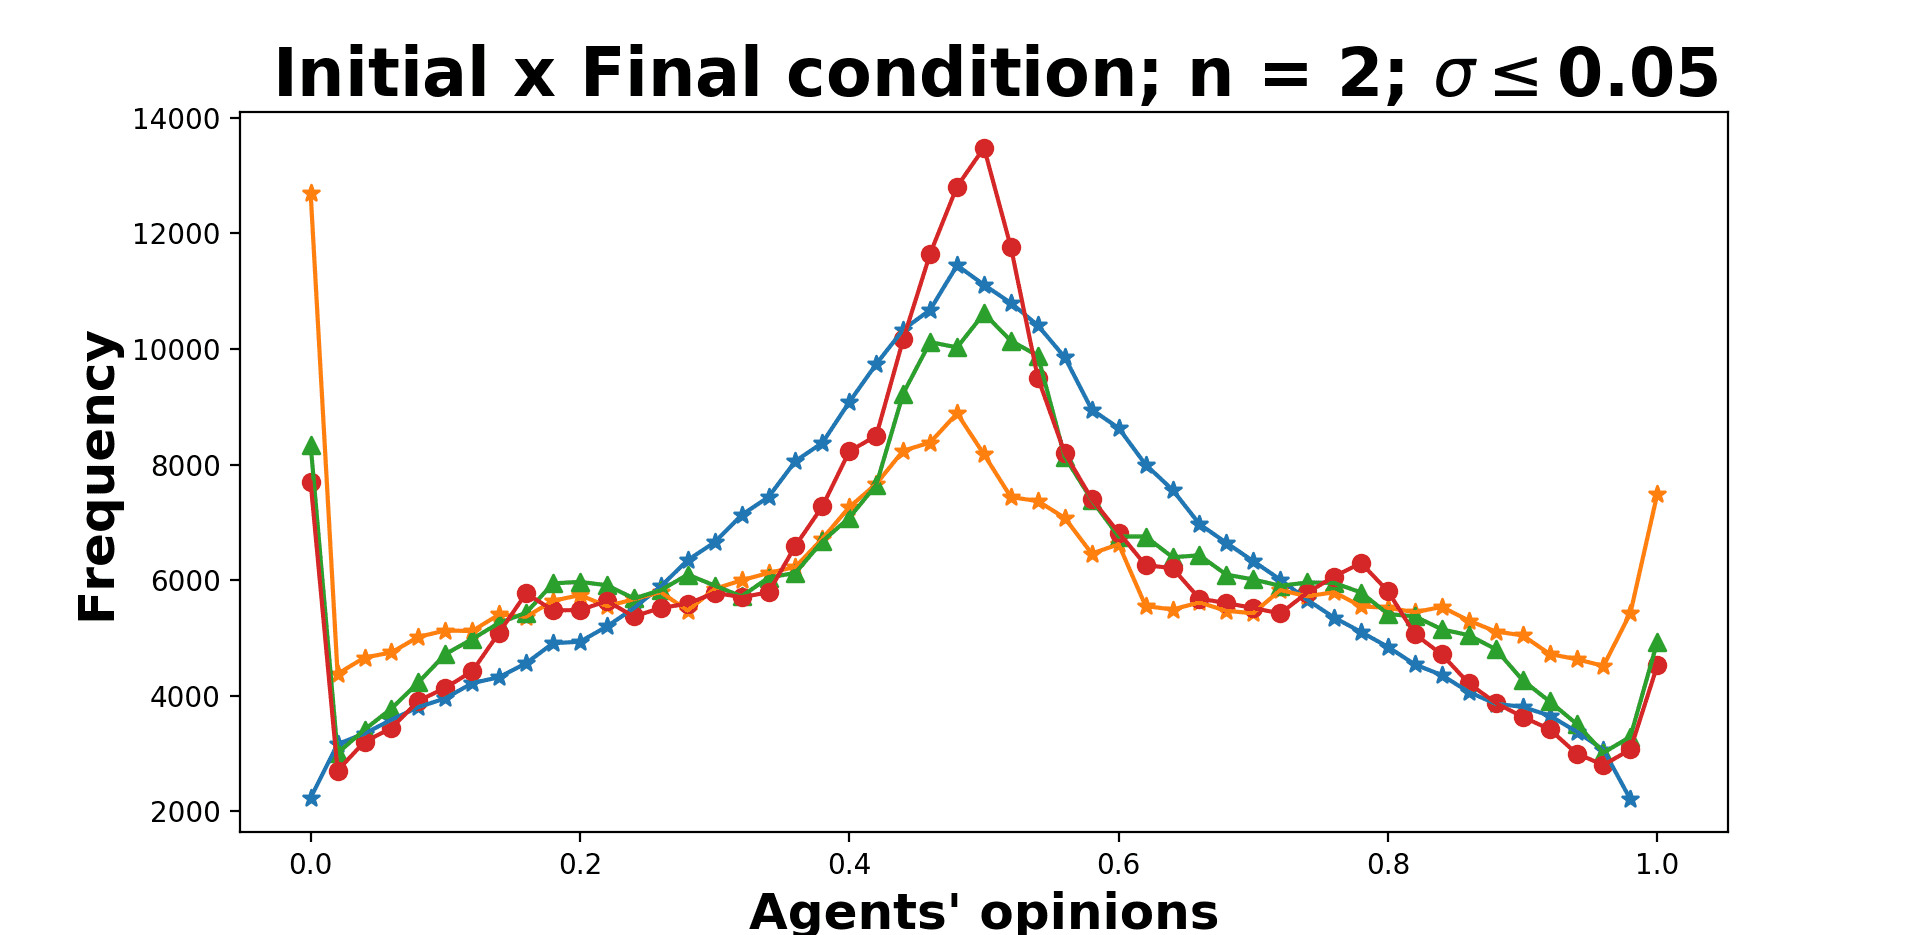
\includegraphics[width=\textwidth]{img/oiks/oiks_smallsigma005_n2.png}
%      \caption{\( n\_issues = 1,  \sigma = 0.1\) }
    \end{subfigure}
         \begin{subfigure}[b]{0.49\textwidth}
      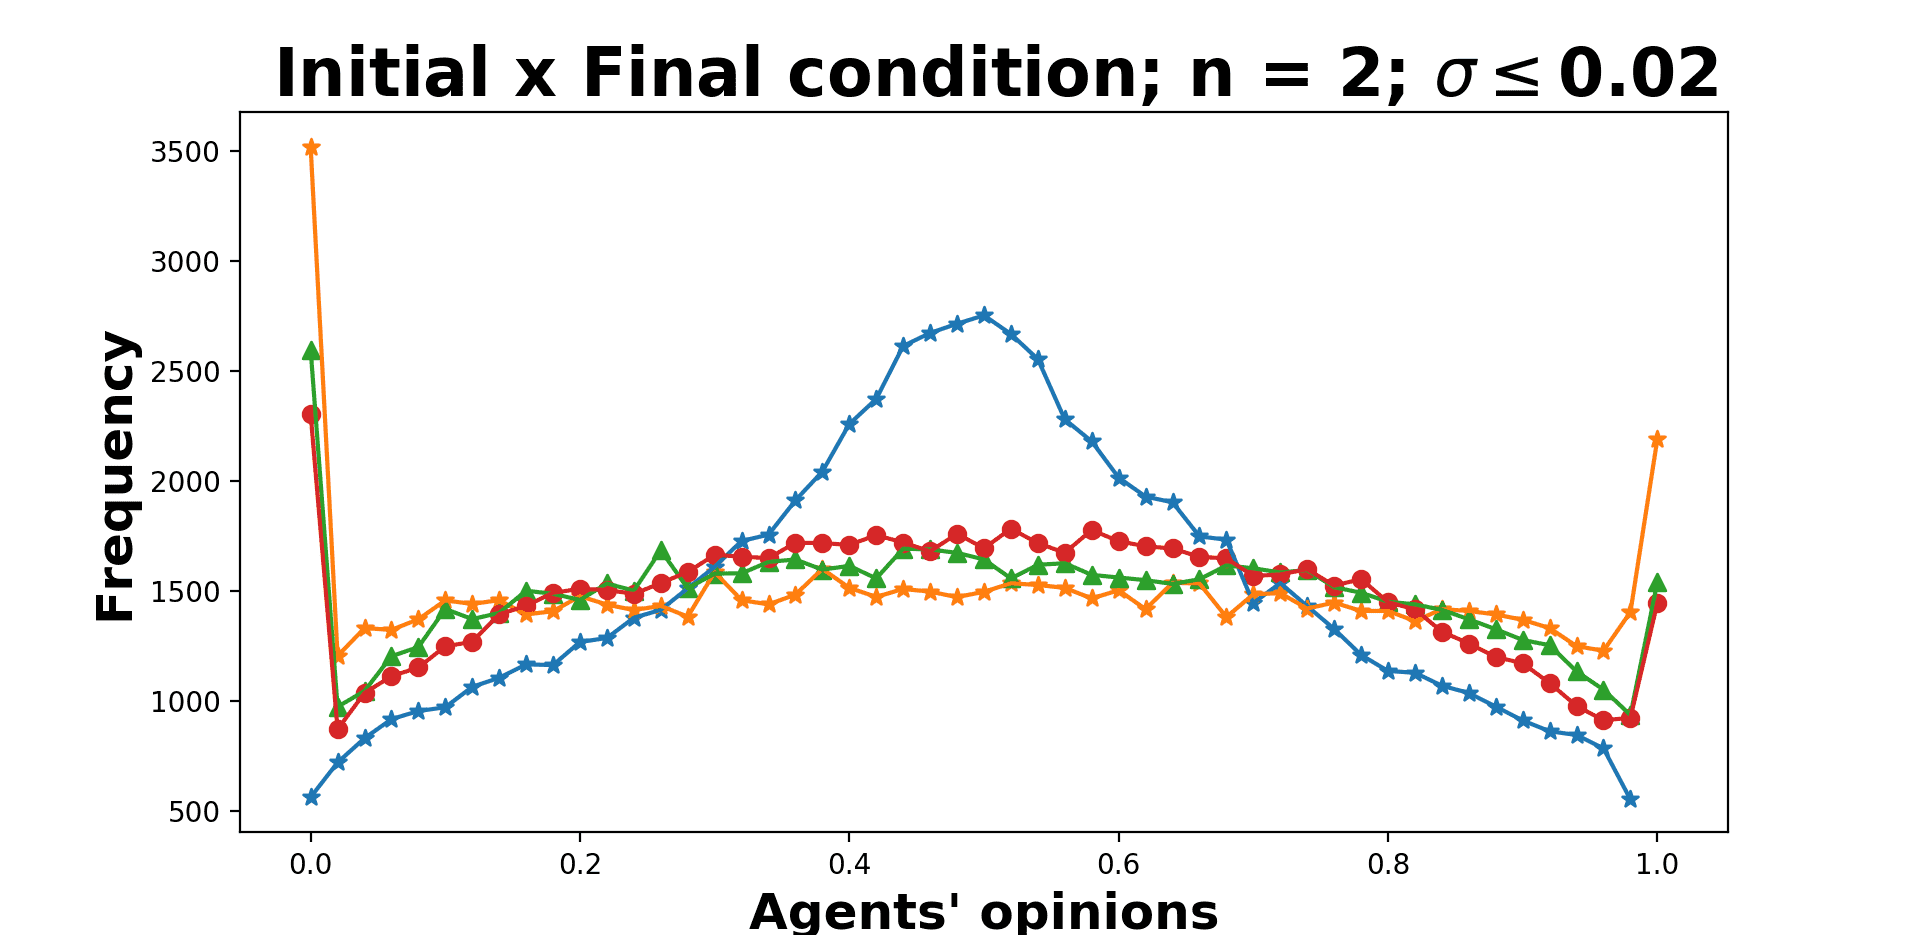
\includegraphics[width=\textwidth]{img/oiks/oiks_smallsigma002_n2.png}
%      \caption{\( n\_issues = 1,  \sigma = 0.1\) }
    \end{subfigure}

    \begin{subfigure}[b]{0.49\textwidth}
      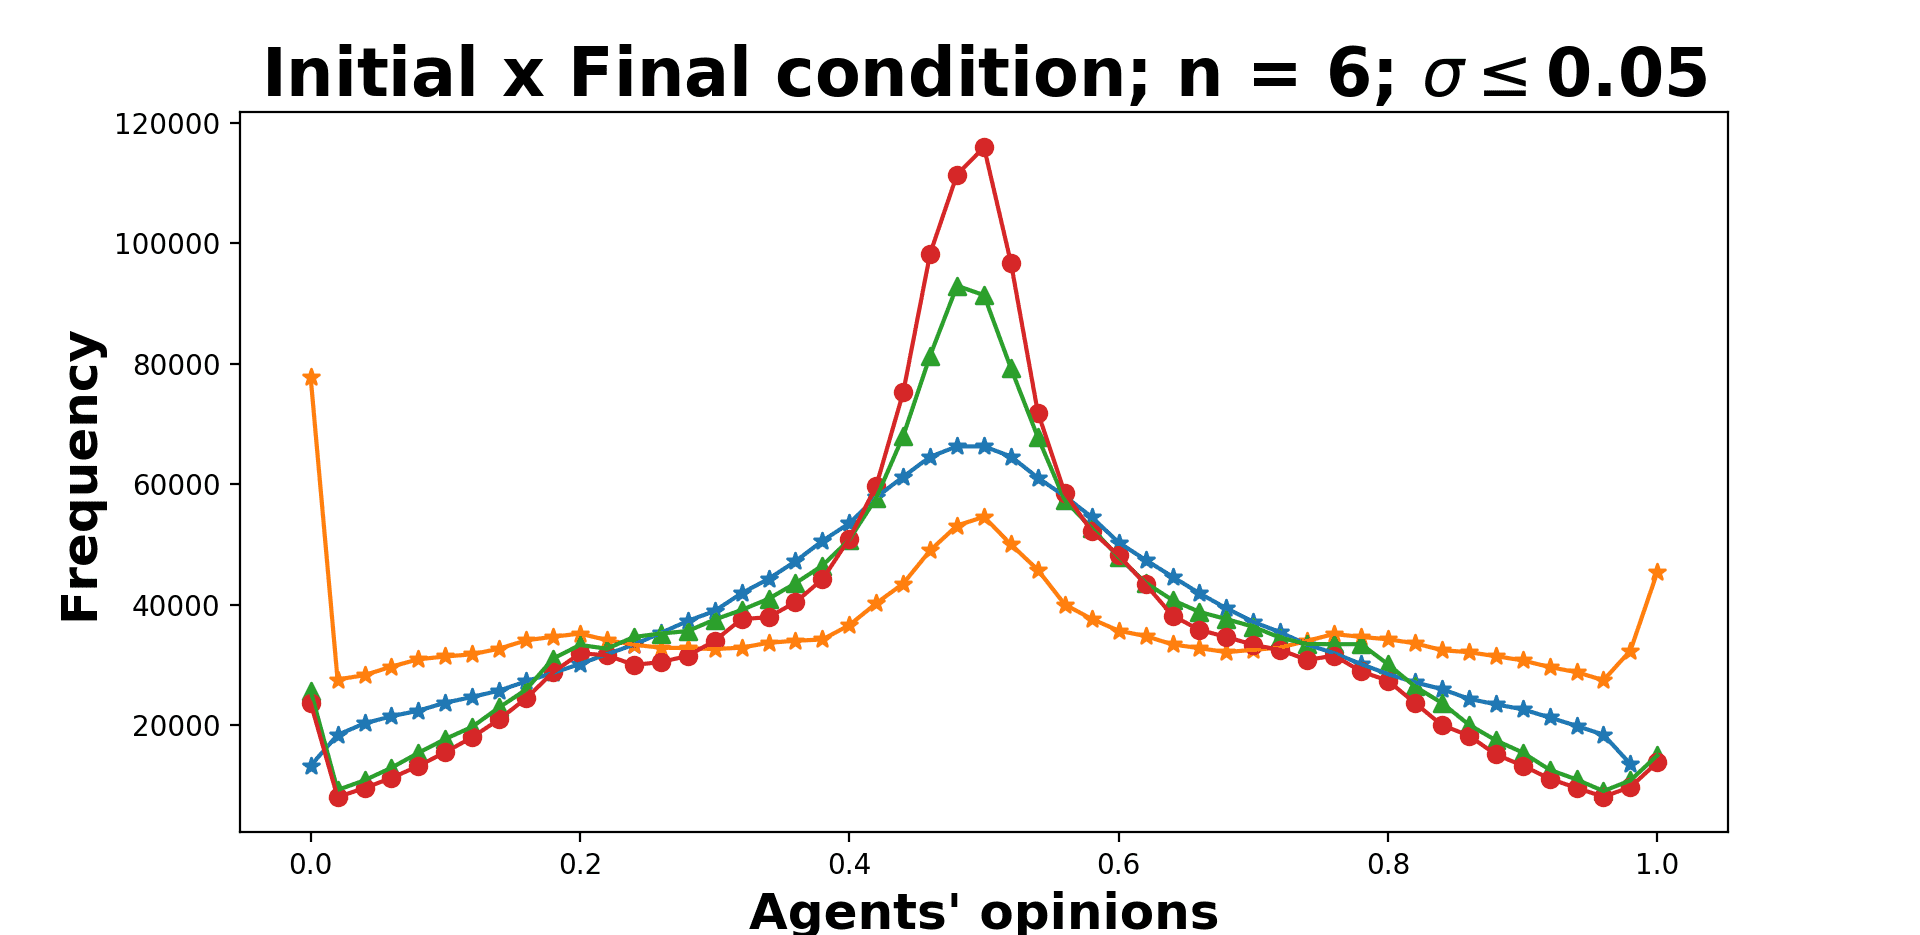
\includegraphics[width=\textwidth]{img/oiks/oiks_smallsigma005_n6.png}
 %      \caption{\(n\_issues = 1, \sigma = 0.02\) }
    \end{subfigure}
    \begin{subfigure}[b]{0.49\textwidth}
      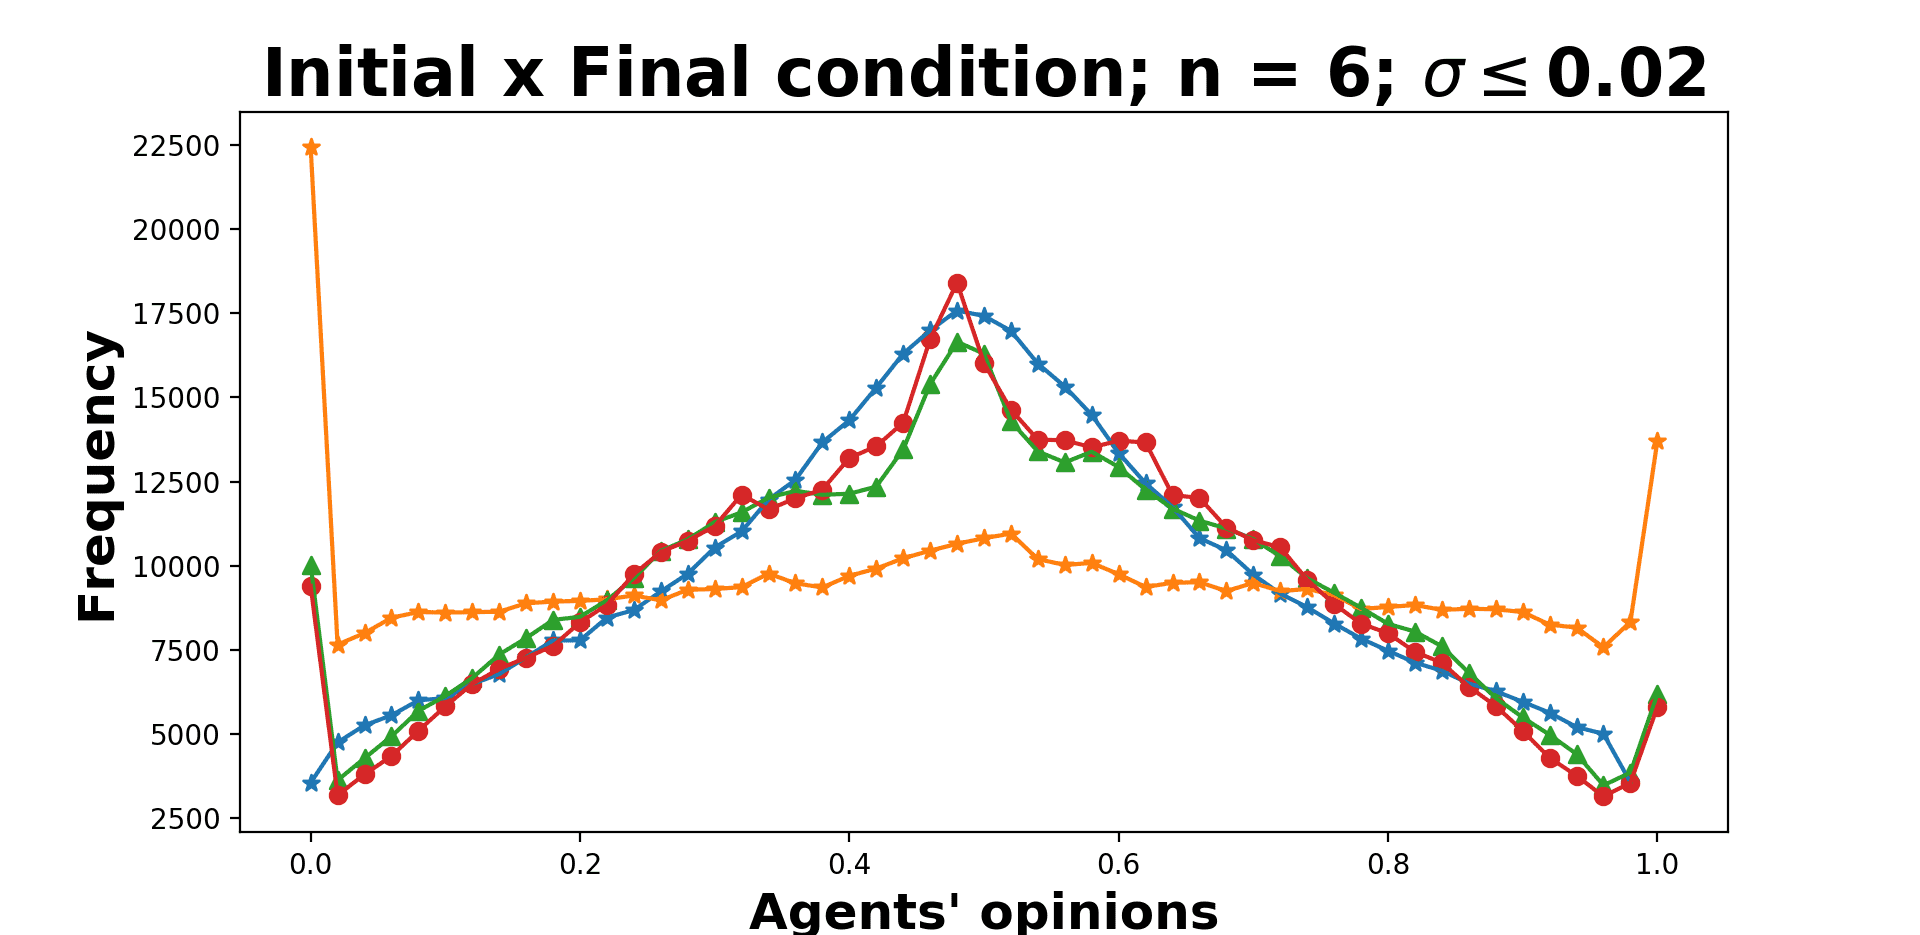
\includegraphics[width=\textwidth]{img/oiks/oiks_smallsigma002_n6.png}
 %      \caption{\(n\_issues = 1, \sigma = 0.02\) }
    \end{subfigure}
     \begin{subfigure}[b]{0.49\textwidth}
       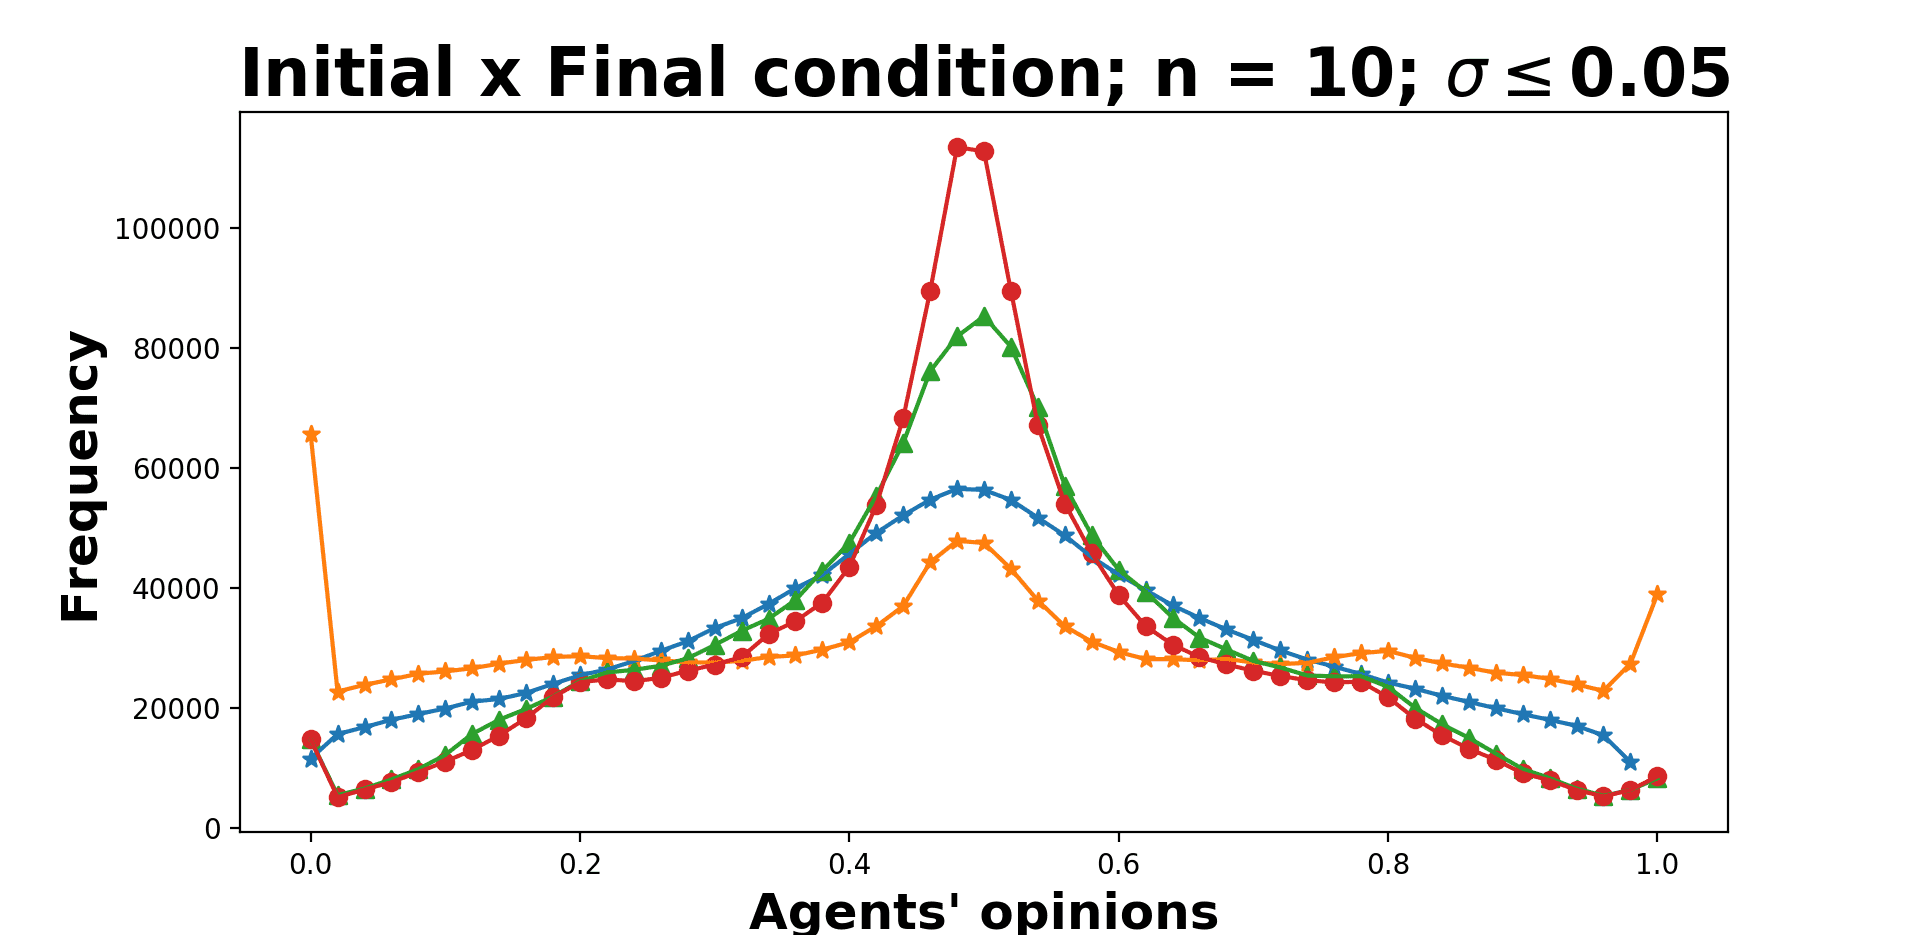
\includegraphics[width=\textwidth]{img/oiks/oiks_smallsigma005_n10.png}
  %     \caption{\(n\_issues = 7, \sigma = 0.1\)}
     \end{subfigure}
     \begin{subfigure}[b]{0.49\textwidth}
       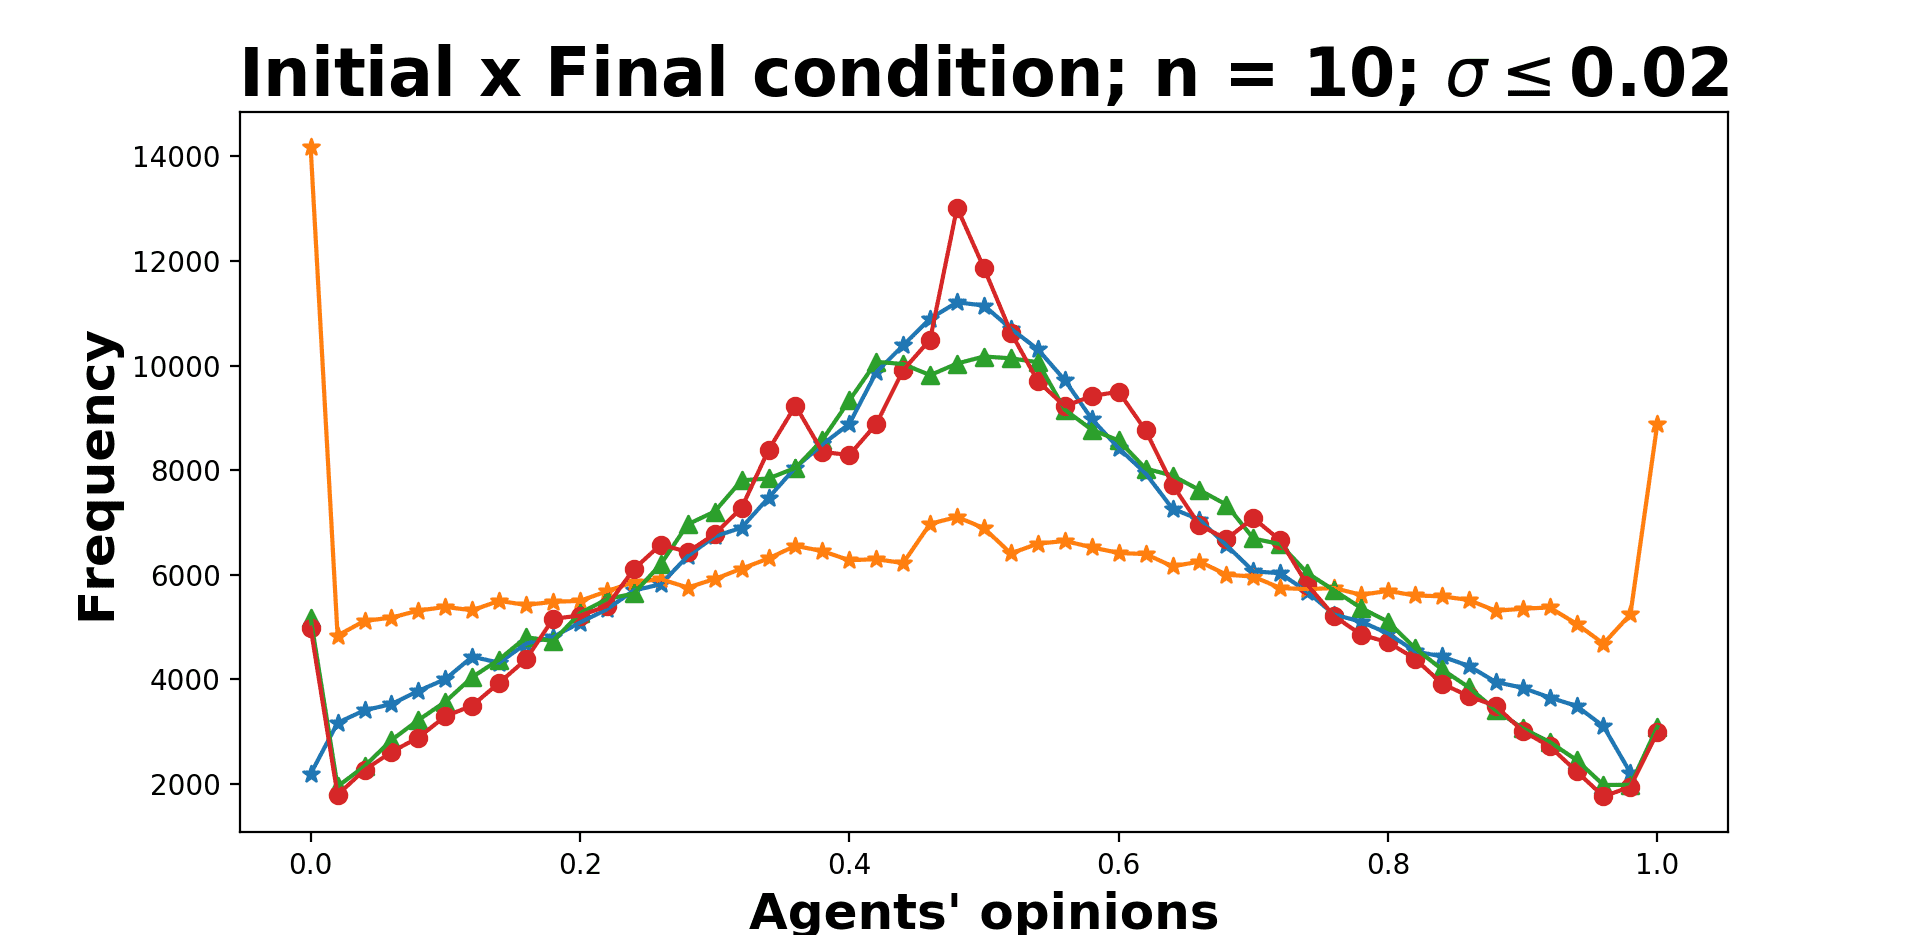
\includegraphics[width=\textwidth]{img/oiks/oiks_smallsigma002_n10.png}
  %     \caption{\(n\_issues = 7, \sigma = 0.1\)}
     \end{subfigure}
     \begin{subfigure}[b]{0.49\textwidth}
       \center
       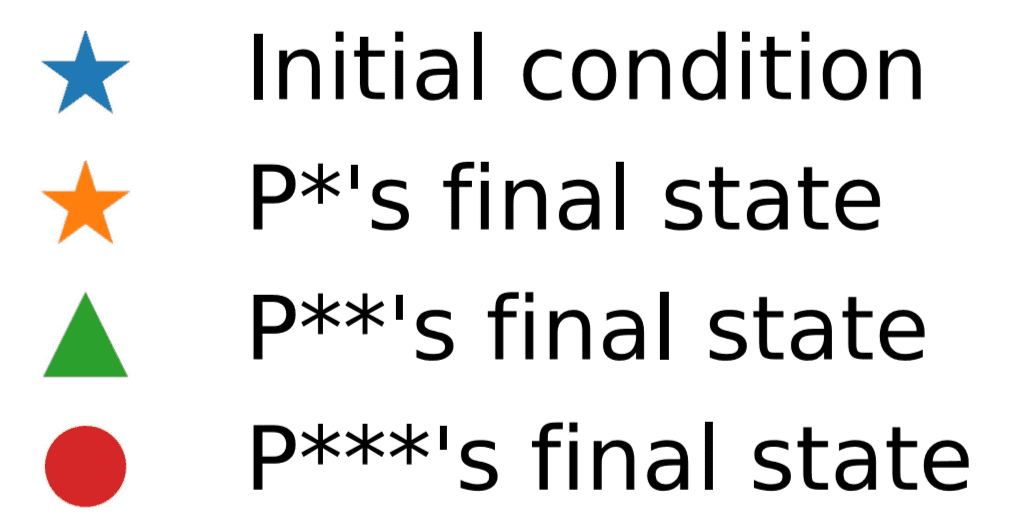
\includegraphics[scale=0.1]{img/oiks/fig2_legend.png}
  %     \caption{\(n\_issues = 7, \sigma = 0.1\)}
     \end{subfigure}

     \caption{Histogram for the final distribution of values of $o_{ik}$.
       Initial distribution is also shown for comparison.}
  \label{fig:oik}
\end{figure}

The behavior of the opinions about specific issues $o_{ik}$ values when we have
small values of $\sigma$ can be observed in the Figure~\ref{fig:oik}. The
graphics show separate cases for different number $n$ of issues and distinct
small values of $\sigma$. The stronger central tendency. While the most
important peak is still around 0.5, the distribution of values is now much more
spread. That reflects the fact that, as $\sigma$ decreases, consensus becomes
much harder and a fraction of the agents find agreement at other values. Indeed,
in every graphic, for the $p^*$ scenario, central opinions become less common
than in initial conditions, while more extreme values become predominant,
showing a clear tendency away from consensus. The same is not true for the more
centralizing versions, $p^{**}$ and $p^{***}$, that seems to show a more varied
behavior. For $\sigma \leq 0.05$, both cases show some tendency to consensus. As
for $\sigma \leq 0.02$, we see very small changes in the initial distribution,
when $n=6$ or $n=10$, and a clear drive to disagreement when $n=2$. In all
scenarios, however, it is clear that the tendency to disagreement is weaker when
update is done following the $p^{**}$ and $p^{***}$ rules than what we observe
for $p^*$.



The histograms, however, don't show the whole story of which parameters
influence the system behavior. With that in mind we performed a Sobol
sensitivity analysis \cite{saltelli2000sensitivity} using as outcome both the
observed standard deviation of agent's mean opinions \(Ystd ^2== \frac{1}{n}
\sum_{k=1}^{n} (x_{i}-\bar{x_i})^2 \) and the standard deviation $S_s$ of the
collection of $N$ internal standard deviations $s_i$. The Sobol indexes
decompose the impact of parameters on the variance of the output. The higher the
value of index the bigger the impact of the parameter on the output. First order
Sobol indexes include linear and non-linear contributions of the parameters,
while total Sobol indexes also include all the interaction effects between
parameters \cite{ten2016sensitivity}. If there are only three parameters, the
total effect \(S_{T1}\) of the first parameter \(X_1\) is given by the equation
\(S_{T1} = S_1 + S_{12} + S_{13} + S_{123}\) where \(S_i =
\frac{V[E(Y|X_i)]}{V(Y)}\); \(S_{12}\) is the impact at the variance of the
output \(Y\) of the interaction of \(X_{1}\) and \(X_{2}\); that is, their
combined effect minus their first order effects: \(S_{ij}\) =
\(\frac{V[E(Y|X_i,X_,)] - V[E(Y|X_i)] - V[E(Y|X_j)]}{V(Y)} \)
\cite{saltelli2008global}. For our simulations, we obtain the estimates:


    \begin{figure}[H]
  \centering
    \begin{subfigure}[b]{0.48\textwidth}
      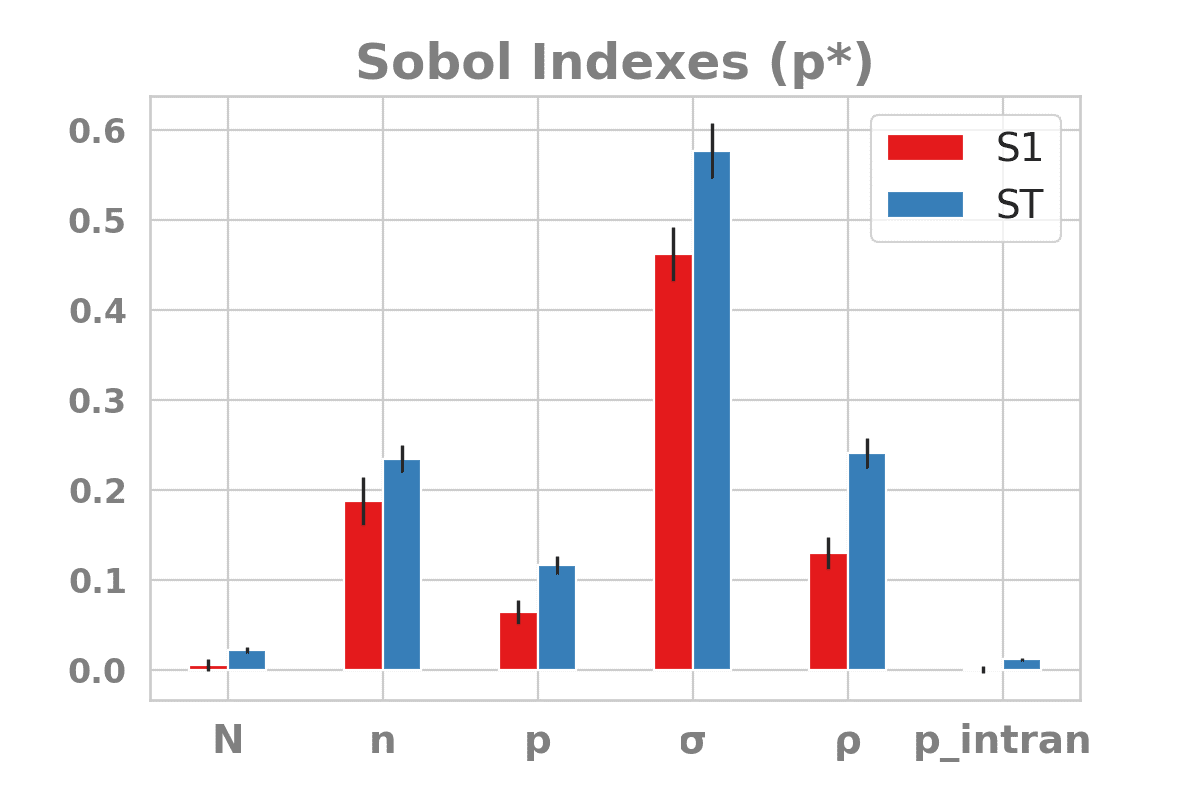
\includegraphics[width=\textwidth]{img/sobolpstar1.png}
%      \caption{\( n\_issues = 1,  \sigma = 0.1\) }
    \end{subfigure}
         \begin{subfigure}[b]{0.48\textwidth}
      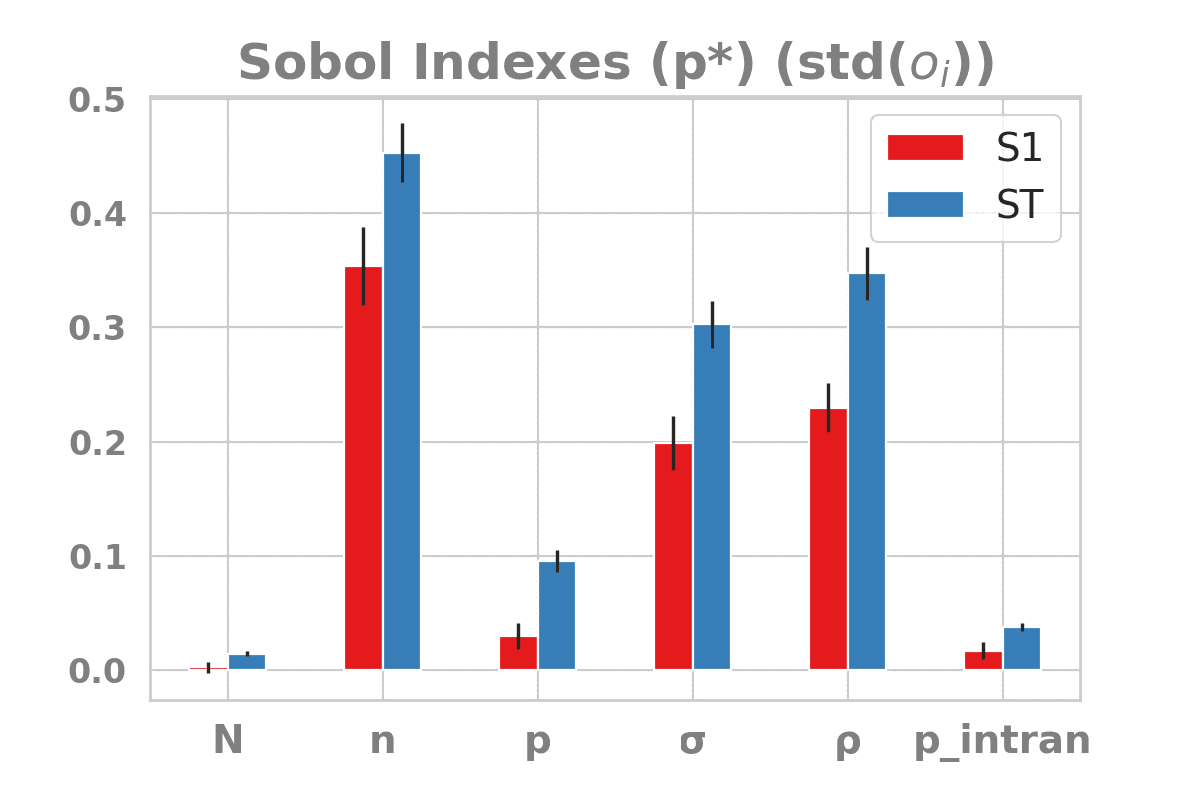
\includegraphics[width=\textwidth]{img/sobolpstar1-measurestd.png}
%      \caption{\( n\_issues = 1,  \sigma = 0.1\) }
    \end{subfigure}
    \begin{subfigure}[b]{0.48\textwidth}
      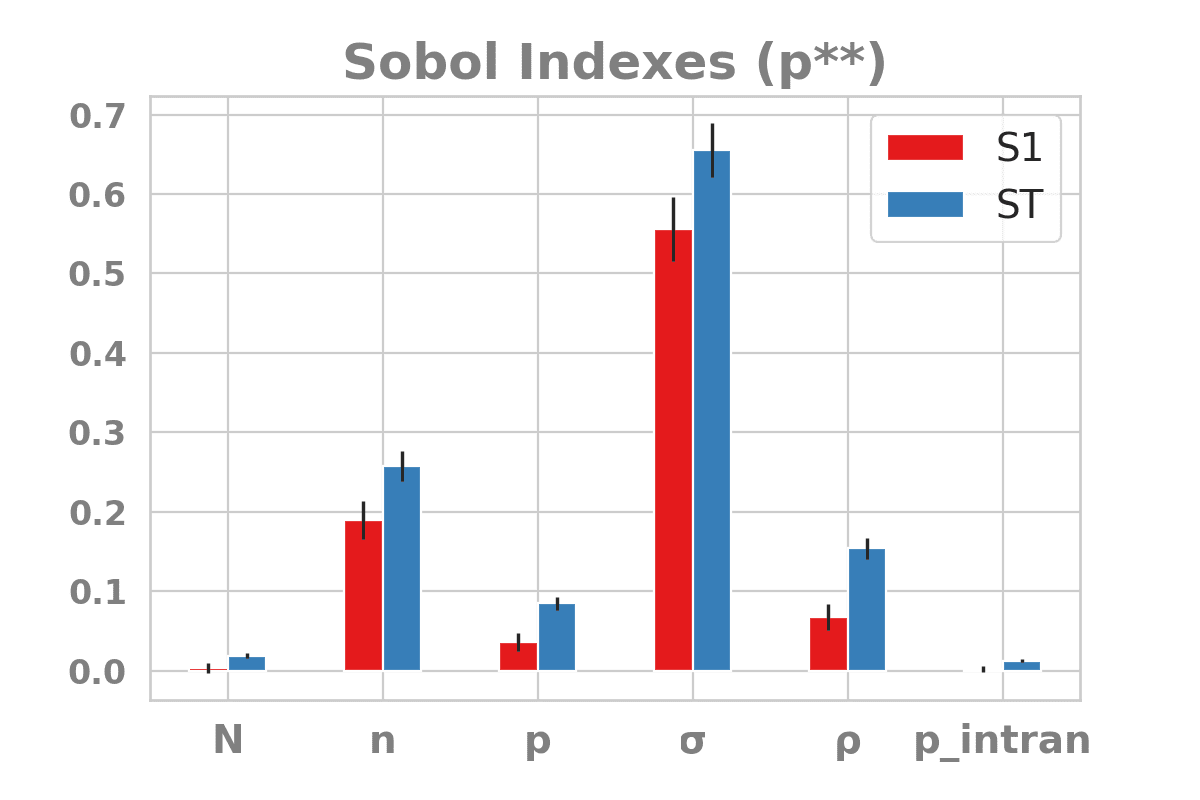
\includegraphics[width=\textwidth]{img/sobolpstar2.png}
 %      \caption{\(n\_issues = 1, \sigma = 0.02\) }
     \end{subfigure}
    \begin{subfigure}[b]{0.48\textwidth}
      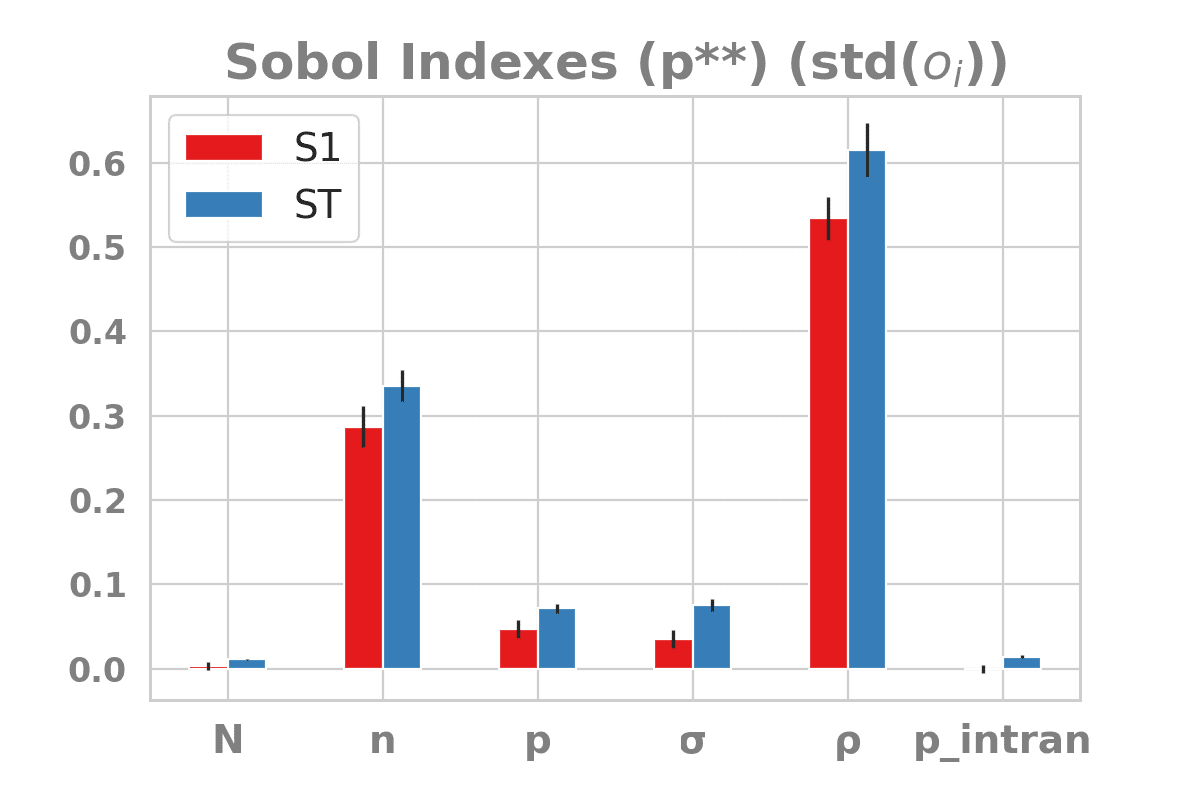
\includegraphics[width=\textwidth]{img/sobolpstar2-measurestd.png}
 %      \caption{\(n\_issues = 1, \sigma = 0.02\) }
     \end{subfigure}
     \begin{subfigure}[b]{0.48\textwidth}
       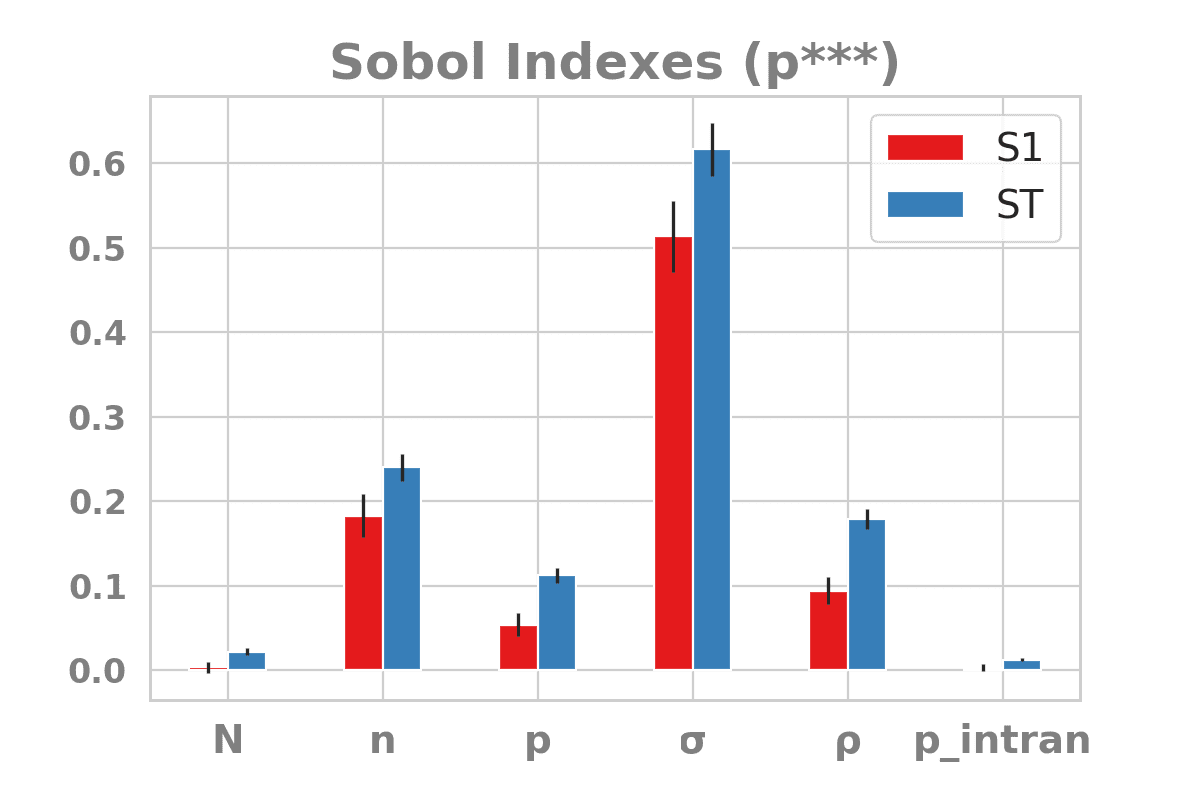
\includegraphics[width=\textwidth]{img/sobolpstar3.png}
  %     \caption{\(n\_issues = 7, \sigma = 0.1\)}
     \end{subfigure}
     \begin{subfigure}[b]{0.48\textwidth}
       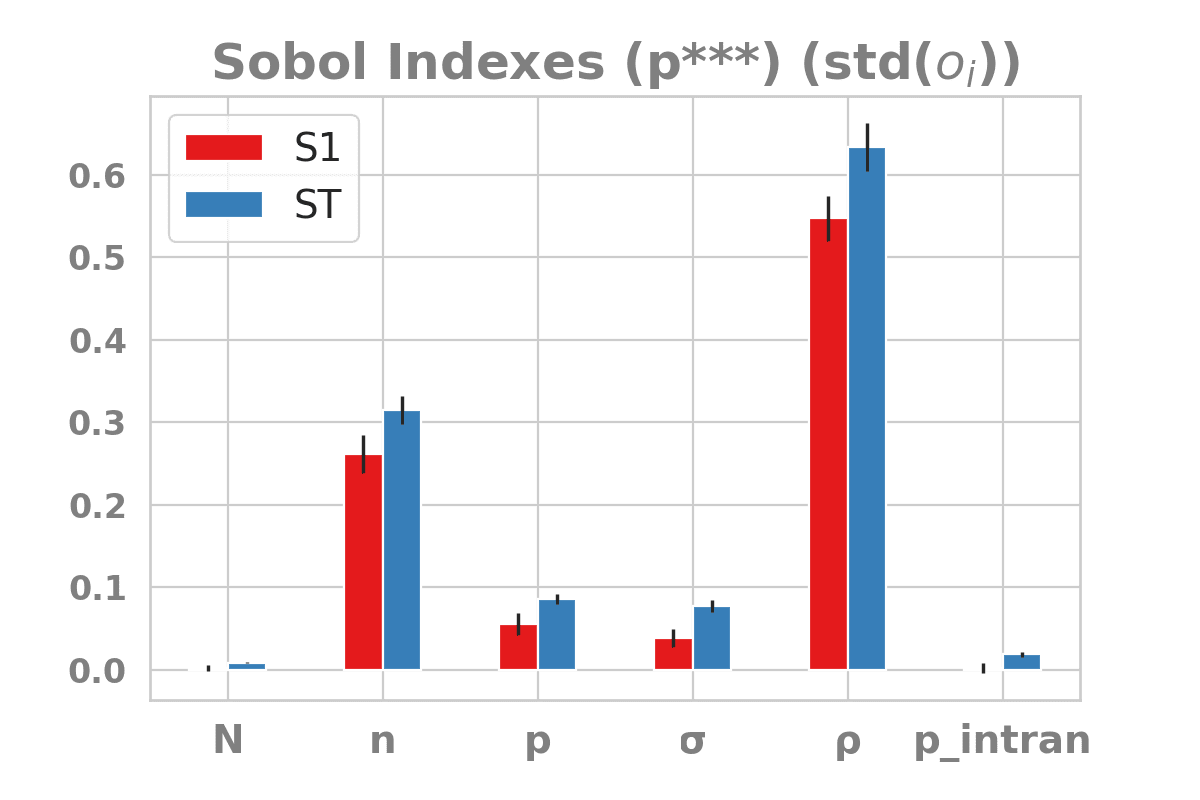
\includegraphics[width=\textwidth]{img/sobolpstar3-measurestd.png}
  %     \caption{\(n\_issues = 7, \sigma = 0.1\)}
     \end{subfigure}
     \caption{Sobol Indexes for the three cases (\(p^{*}, p^{**}, p^{***}\)). First column shows the analysis for $Ystd$ and the second column, for $S_s$.}
     \label{fig:sobol}
    \end{figure}

    The sensitivity analysis in Figure\ref{fig:sobol} shows that \(\sigma, n \),
    and \(\rho\) have the most influence on the final values of $Ystd$ and
    $S_s$. $p$ seems to still have some smaller influence and both $N$ and
    $p_{intran}$ seem to make no difference for the range of values we used. It
    is also interesting to notice that the same general behavior appears in the
    three scenarios for $Ystd$. \(\sigma\) being the parameter that explains
    most of the variance was expected and it is consistent with
    \citep{martins12b}. It is interesting to see that two of the new parameters,
    the number of issues $n$ and the noise \(\rho\), also play an important role
    in explaining the total variance of $Ystd$.

    When we look at the standard deviation of the agent's opinions, $S_s$,
    however, we see that \(\sigma\) is the most relevant parameter only for the
    $p^*$ case. For $p^{**}$ and $p^{***}$, however, \(\sigma\) seems to matter
    very little, basically as much as $p$. And the noise $\rho$ seems to have
    most of the impact on $S_s$. This change is not so hard to understand. As we
    are speaking of how much change we observe in the standard deviations of
    each agent opinions $s_i$, there is a fundamental difference between the
    $p^*$ scenario and the $p^{**}$ and $p^{***}$ ones. On the first one, the
    opinion of $i$ in each issue does not depend on its own opinion on other
    issues. However, as in both $p^{**}$ and $p^{***}$ agent $i$ uses its own
    mean to decide own much to trust other agents, it is natural $i$ opinions
    will tend to a mean value. So, while for $p^*$, $s_i$ is driven by how much
    the opinions get spread in general and, therefore, by \(\sigma\) , $p^{**}$
    and $p^{***}$ scenarios suggest that the tendency to keep consistent
    opinions predominates and the variation in the final results is driven
    mostly by the noise. This is compatible with what we observed Figure
    \ref{fig:std} for the distribution of $s_i$. There, we had that the $p^*$
    showed it was common to observe agents with very little internal
    consistency, equivalent to large amounts of $s_i$. The tail for high $s_i$,
    however, was significantly smaller for $p^{**}$ and $p^{***}$, with
    $p^{***}$ even showing cases where very small $s_i$ became more frequent
    than in the initial distribution.


    A sensitivity analysis, however, does not show the direction of the impact.
    Figure~\ref{fig:scatters} shows scatter plots for $Ystd$ as a function of
    the main parameters. Each point corresponds to the outcome of one
    implementation of the model for the value of the parameter at the $x$-axis
    and the observed value of $Ystd$. Similar scatter plots for $S_s$ showed
    similar behaviors and, therefore, are not shown here.

        \begin{figure}[H]
  \centering

    \begin{subfigure}[b]{0.48\textwidth}
      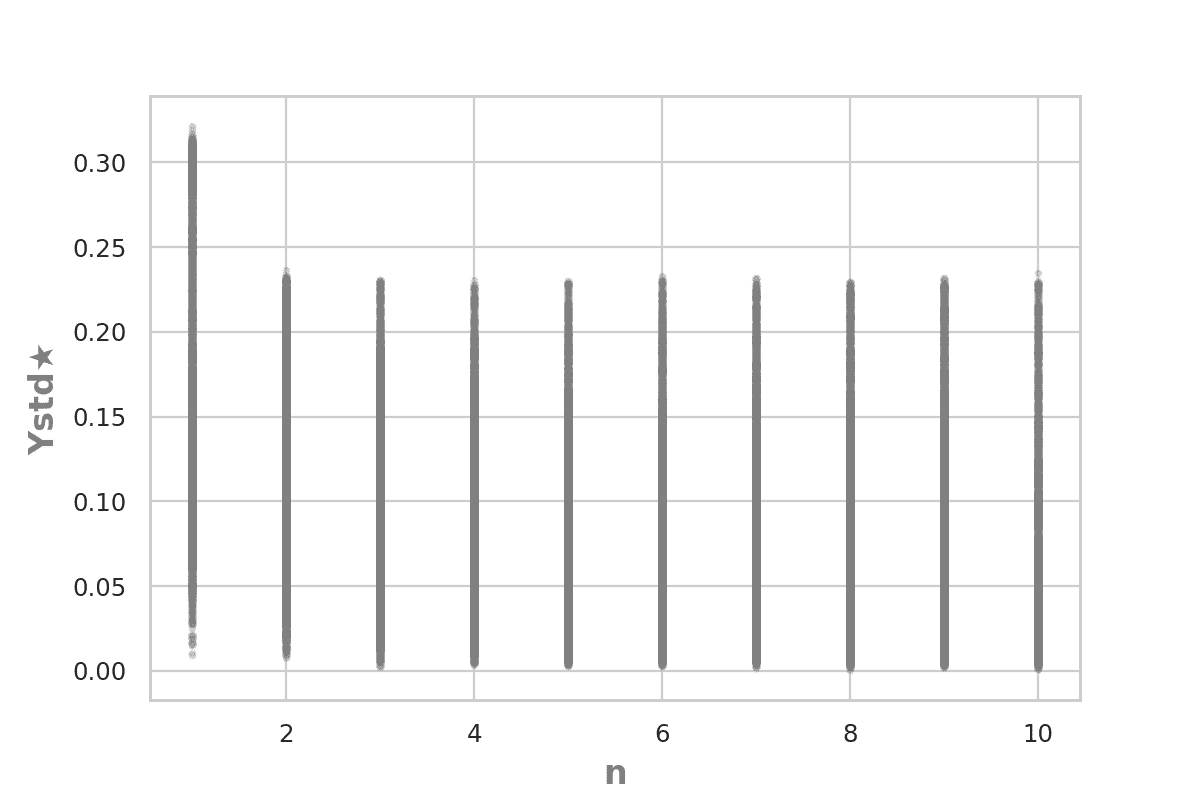
\includegraphics[width=\textwidth]{img/regressionYstdsn.png}
    \end{subfigure}
    \begin{subfigure}[b]{0.48\textwidth}
      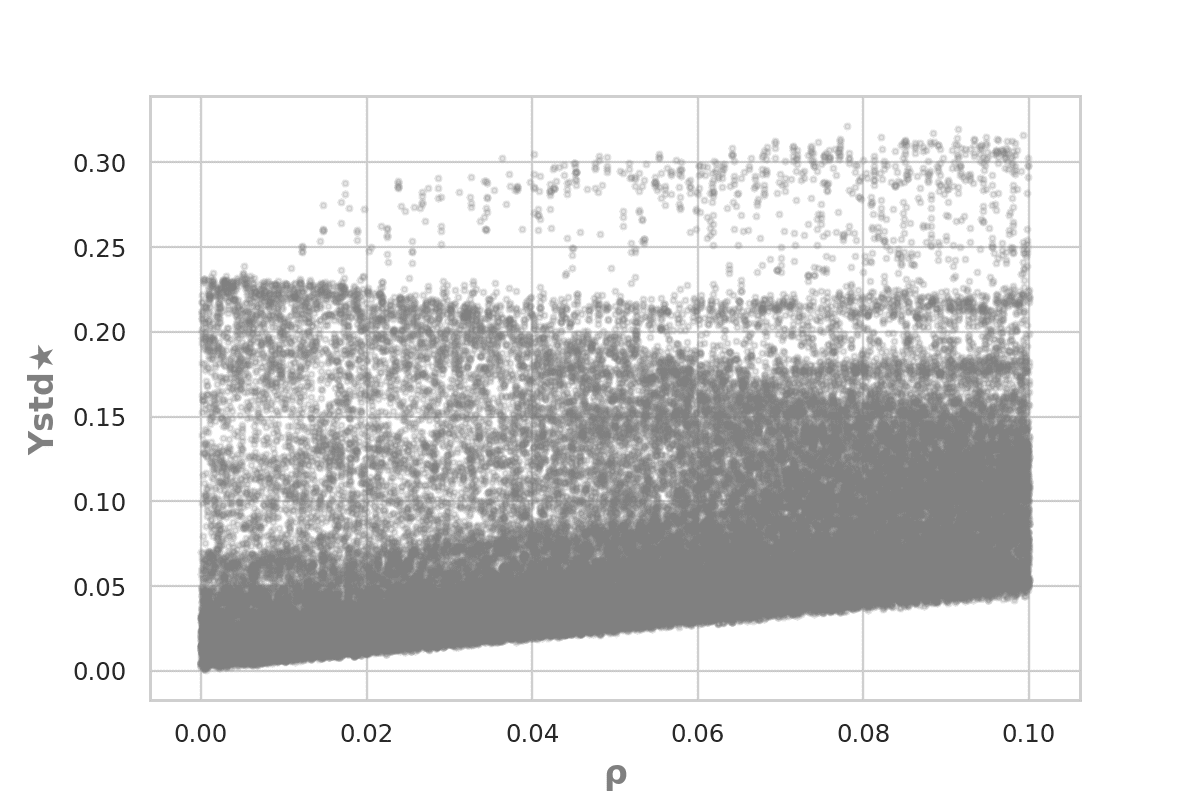
\includegraphics[width=\textwidth]{img/regressionYstdsrho.png}
 %      \caption{\(n\_issues = 1, \sigma = 0.02\) }
     \end{subfigure}
     \begin{subfigure}[b]{0.5\textwidth}
       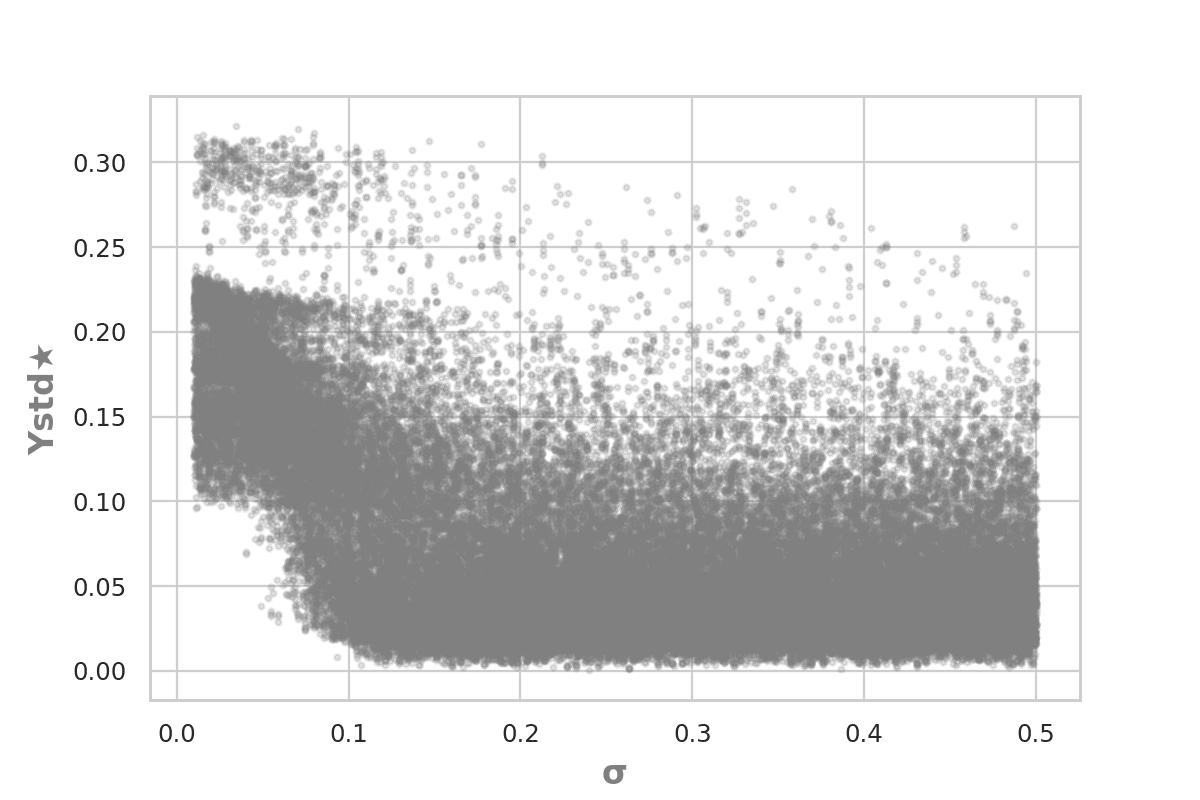
\includegraphics[width=\textwidth]{img/regressionYstdssigma.png}
  %     \caption{\(n\_issues = 7, \sigma = 0.1\)}
     \end{subfigure}
     \caption{Scatterplots for the parameters with highest impact. Each dot corresponds to the result obtained in a single run.}
      \label{fig:scatters}
    \end{figure}


    The negative impact of \(\sigma\) in the population' opinion dispersion is
    expected: a higher \(\sigma\) means agents are easier to influence. As they
    are connected to all the other agents, the more uncertain they are, the more
    centralized the agents' mean opinions will tend to become. The plots also
    show that the exact value of \(\sigma\) seems to matter little above
    approximately 0.1. Therefore we restrict our following analysis to
    \(\sigma\) in the \((0.0, 0.1 ] \) range. The effect of \(\rho\) is also
    expected: the bigger the noise, the more dispersed the final state of the
    system is. The number of issues $n$ seems to have little influence unless it
    is $n=1$. When there is only one issue, we see scenarios where the opinions
    clearly move away to stronger polarizations, with (\(Ystd\)) around 0.3.
    Those cases are no longer observed as we have at least two issues. That is
    probably an artifact of initial conditions. As initial conditions were
    randomly drawn, extreme values in all issues become more and more rare with
    increasing number of issues $n$ and, therefore, there are very few agents to
    push others to the more extreme regions.


    Now we have a general picture, looking at typical behaviors for specific
    parameter values helps us understand the model better. We ran cases where we
    kept \(\rho = 0.05 \) ; \(N = 500\) ; \(p\_intran = 0.0\) fixed, for 500.000
    iterations, and test combinations of $\sigma = (0.02, 0.04, 0.1)$ and $ n =
    (1,5,10)$. The time series at Figure \ref{fig:tseries1} show the time
    evolution of the opinions of all $500$ agents for a typical run of the the
    $p{***}$ case. Only results for $p{***}$ are shown here because the time
    series for $p^*$ and $p{**}$ are visually almost identical to the ones in
    the figures. We see that larger values \(\sigma\) seem to lead opinions
    towards the center: the bigger the \(\sigma\) is, the more agents will tend
    to move closer to the mean.


        \begin{figure}[H]
  \centering
       \begin{subfigure}[b]{0.48\textwidth}
      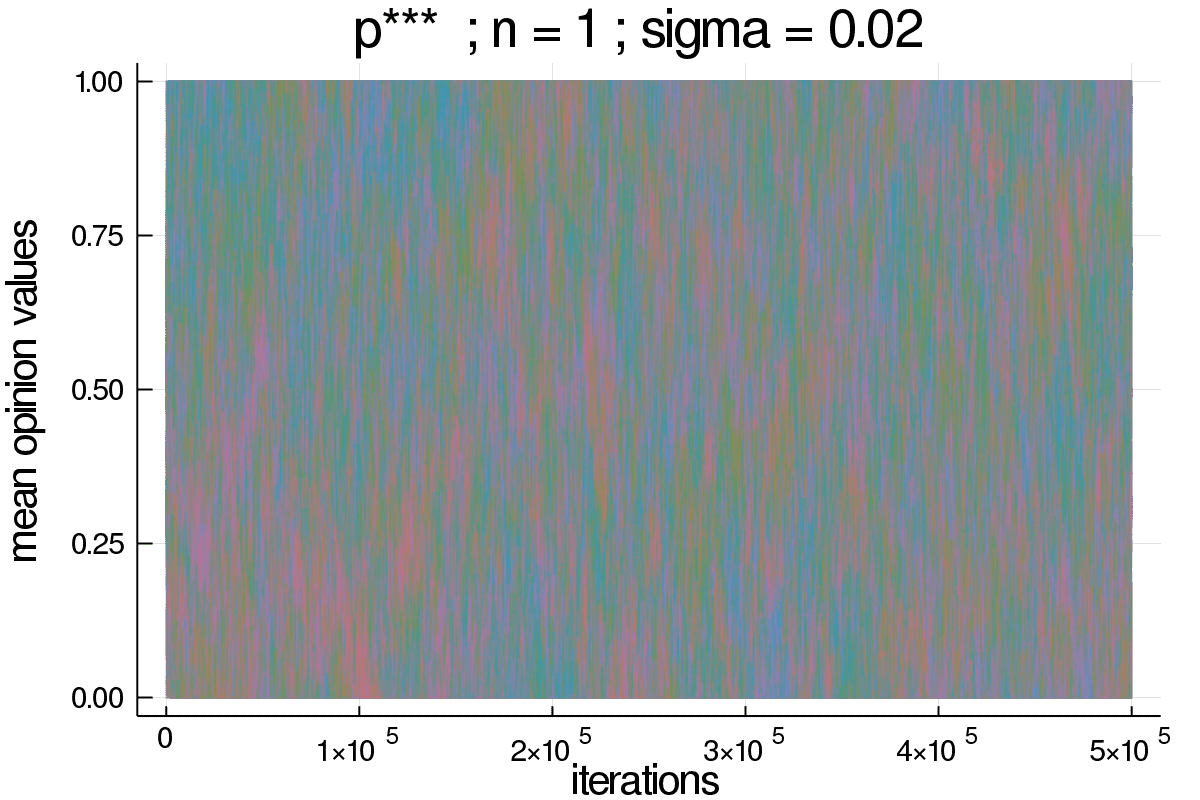
\includegraphics[width=\textwidth]{img/series/tseries1/Poodlcalculatepsssn1-rho005-sigma002-00intransrandom.png}
 %      \caption{\(n\_issues = 1, \sigma = 0.02\) }
     \end{subfigure}
    \begin{subfigure}[b]{0.48\textwidth}
      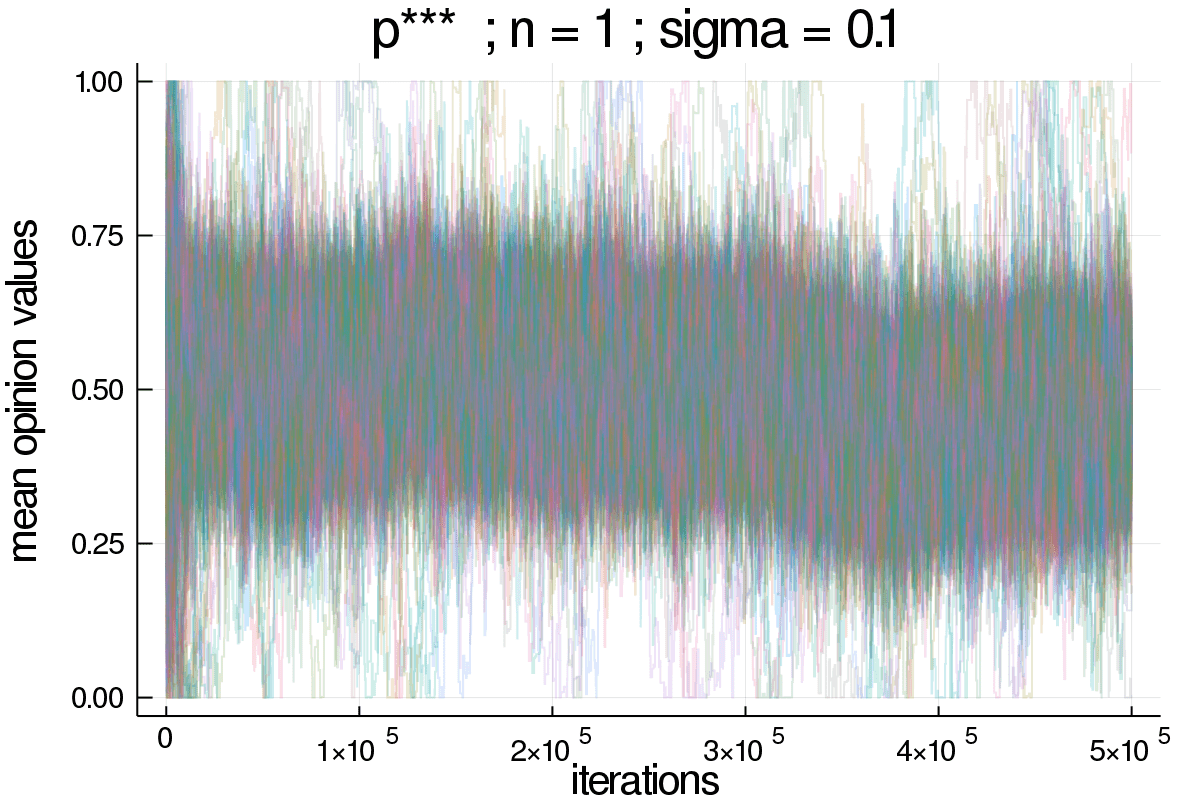
\includegraphics[width=\textwidth]{img/series/tseries1/Poodlcalculatepsssn1-rho005-sigma01-00intransrandom.png}
      %\caption{\textcolor{red}{'ill fix thix}}
    \end{subfigure}
              \begin{subfigure}[b]{0.48\textwidth}
      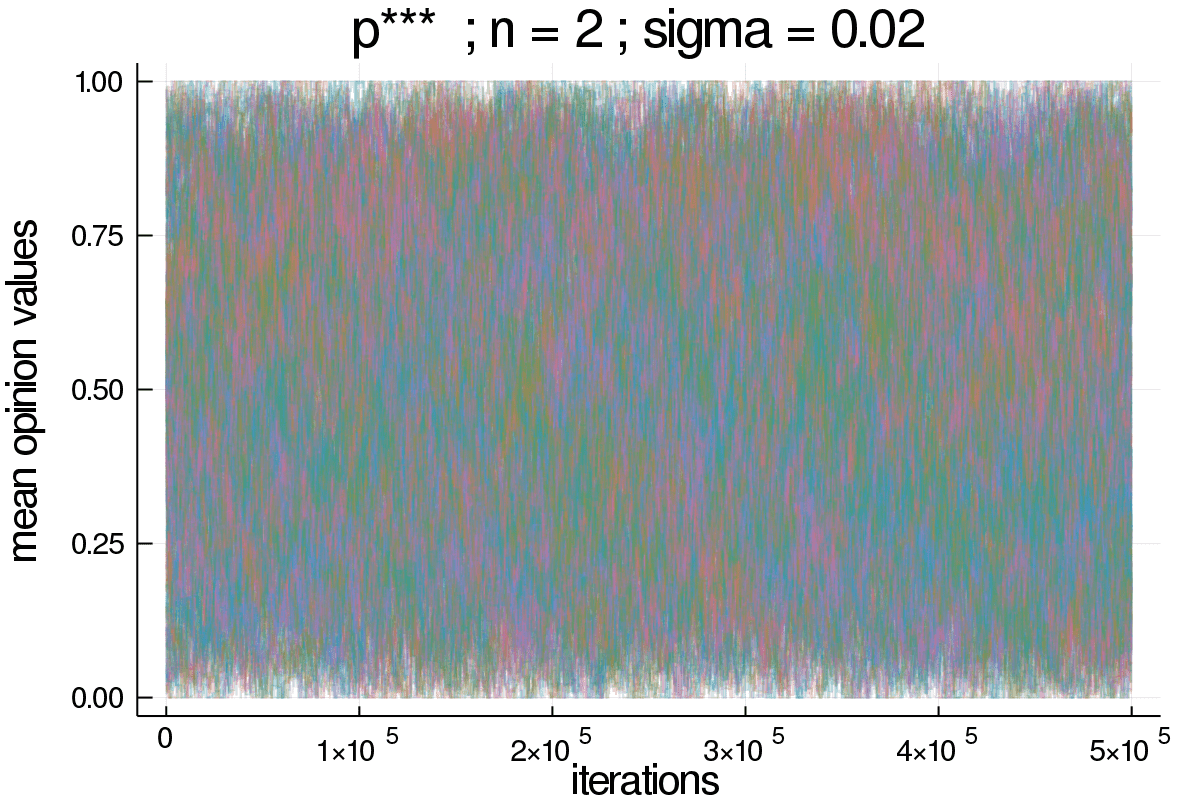
\includegraphics[width=\textwidth]{img/series/tseries1/Poodlcalculatepsssn2-rho005-sigma002-00intransrandom.png}
 %      \caption{\(n\_issues = 1, \sigma = 0.02\) }
     \end{subfigure}
    \begin{subfigure}[b]{0.48\textwidth}
      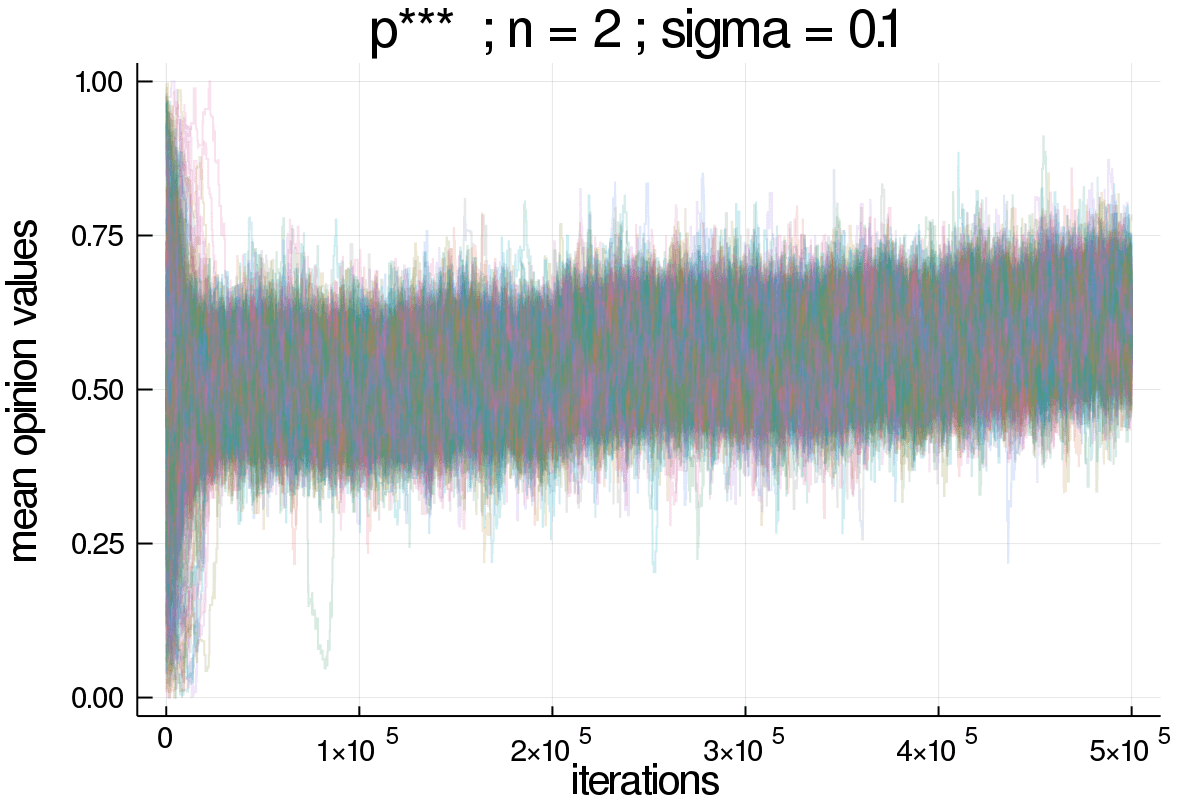
\includegraphics[width=\textwidth]{img/series/tseries1/Poodlcalculatepsssn2-rho005-sigma01-00intransrandom.png}
 %      \caption{\(n\_issues = 1, \sigma = 0.02\) }
    \end{subfigure}
     % \begin{subfigure}[b]{0.48\textwidth}
     %   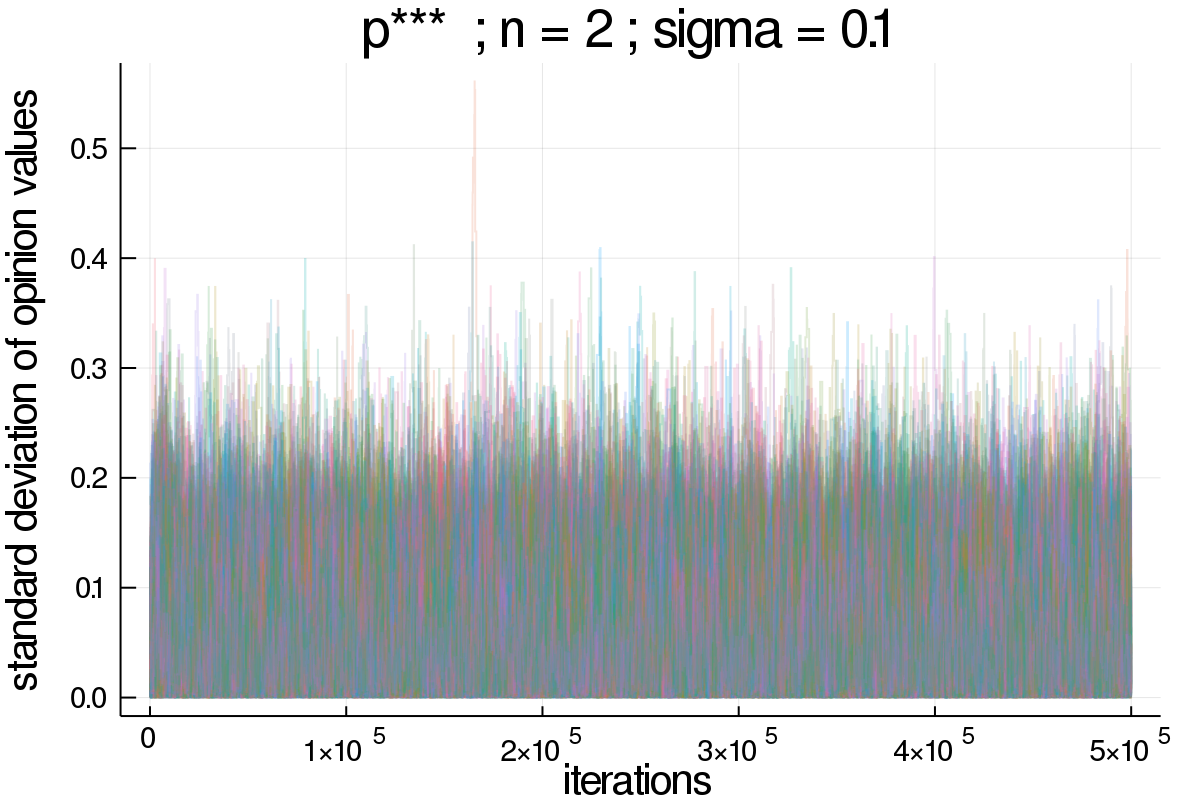
\includegraphics[width=\textwidth]{img/series/tseries1/Poodlcalculatep***n2-rho005-sigma01-00intransrandom-std.png}
     % \end{subfigure}
%     \begin{subfigure}[b]{0.48\textwidth}
%       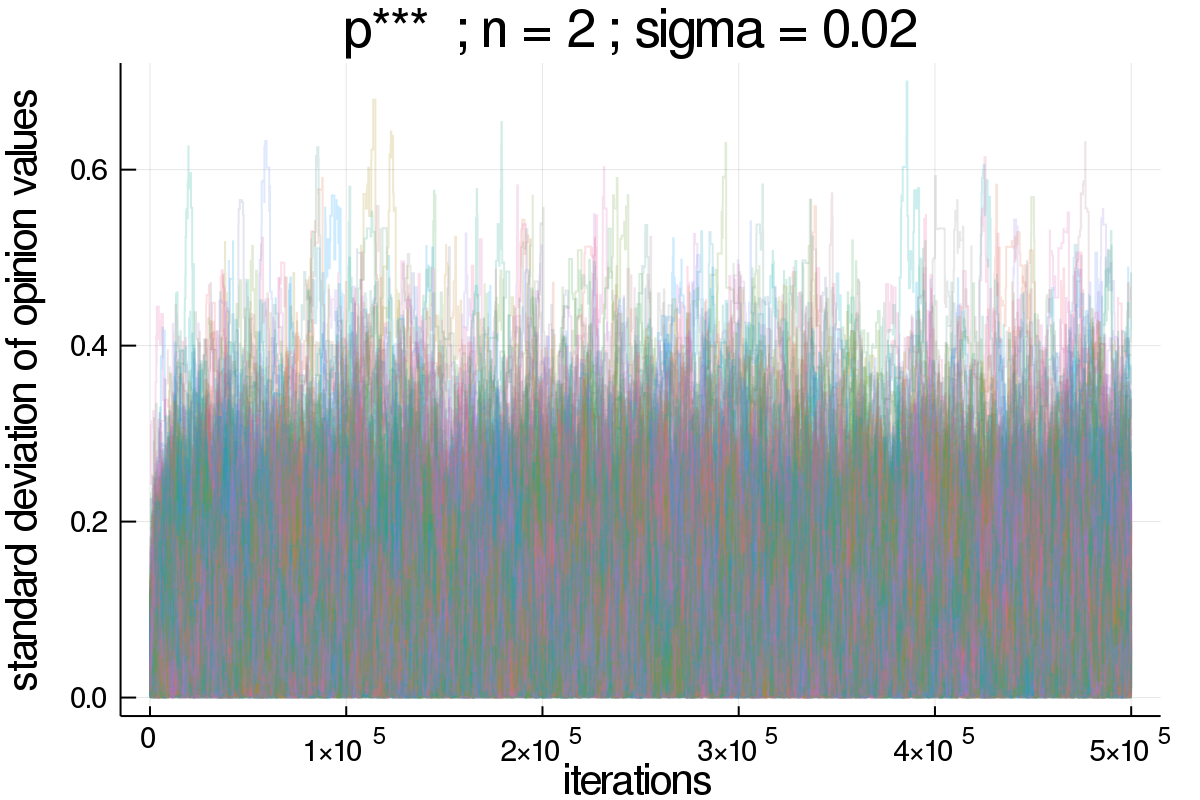
\includegraphics[width=\textwidth]{img/series/tseries1/Poodlcalculatep***n2-rho005-sigma002-00intransrandom-std.png}
% %     \caption{\(n\_issues = 7, \sigma = 0.1\)}
%      \end{subfigure}
     \caption{Time series for the parameterization: \(\rho = 0.05, N = 500,
       p\_intran = 0.0, n  = 1 \) or  $2$}
      \label{fig:tseries1}
    \end{figure}





    Figure \ref{fig:tseries2} shows a similar time evolution series for $n=5$
    issues. Here, even for small values of $\sigma$ we observe the opinions tend
    to avoid the more extreme values. As commented before, that seems to be an artifact of initial
    random draws. While it is easy to draw the most extreme values with only one
    draw, for $n=5$, as we are close to the end of the range, no values outside
    that range are possible. So, the most extreme values require that, at the
    start, agents should have all their five issues drawn as extreme. As that is
    rare, those few that do start there tend to be attracted to still extreme
    positions, but a little less so. However, there actually seems to be a stronger
    tendency towards more central opinions. That can be observed as the increase in $\sigma$
    leads to a position closer to consensus than we observed in Figure \ref{fig:tseries1} for the $n=1$ case.





    \begin{figure}[H]
      \centering
      \begin{subfigure}[b]{0.48\textwidth}
        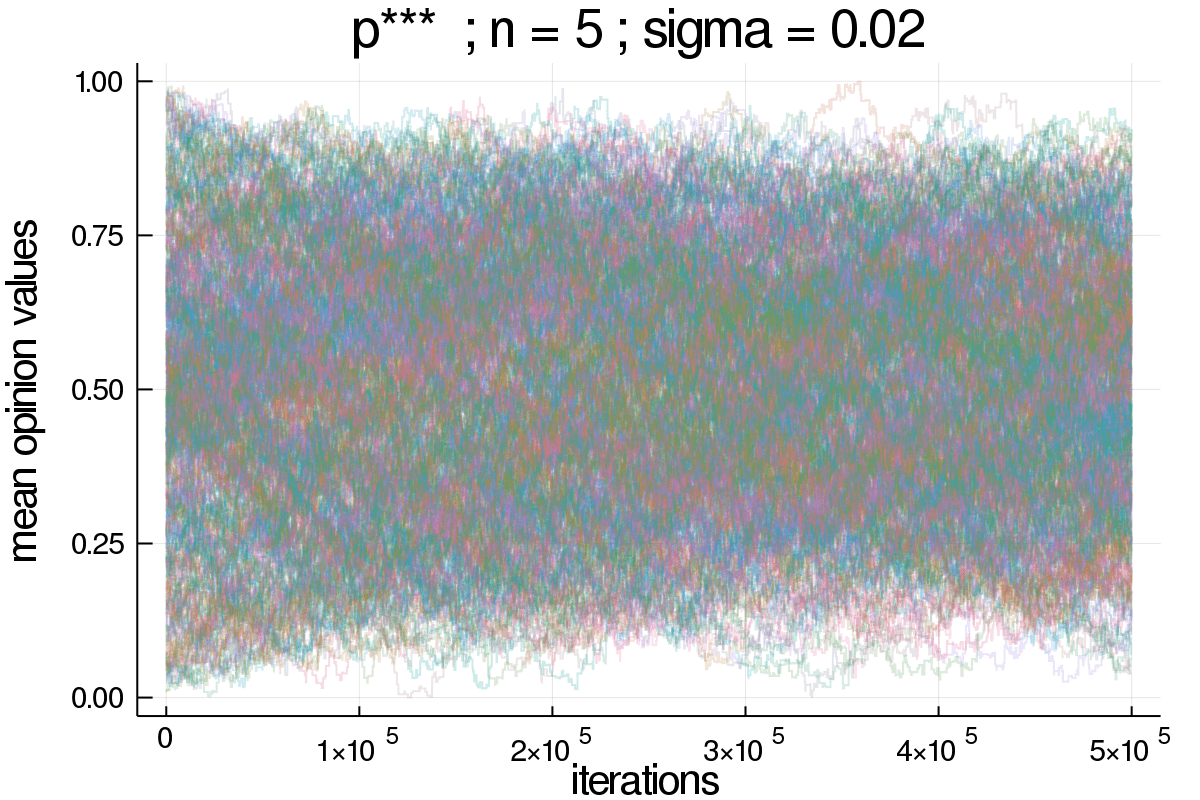
\includegraphics[width=\textwidth]{img/series/tseries2/Poodlcalculatepsssn5-rho005-sigma002-00intransrandom.png}
        % \caption{\textcolor{red}{'ill fix thix}}
      \end{subfigure}
%           \begin{subfigure}[b]{0.48\textwidth}
 %       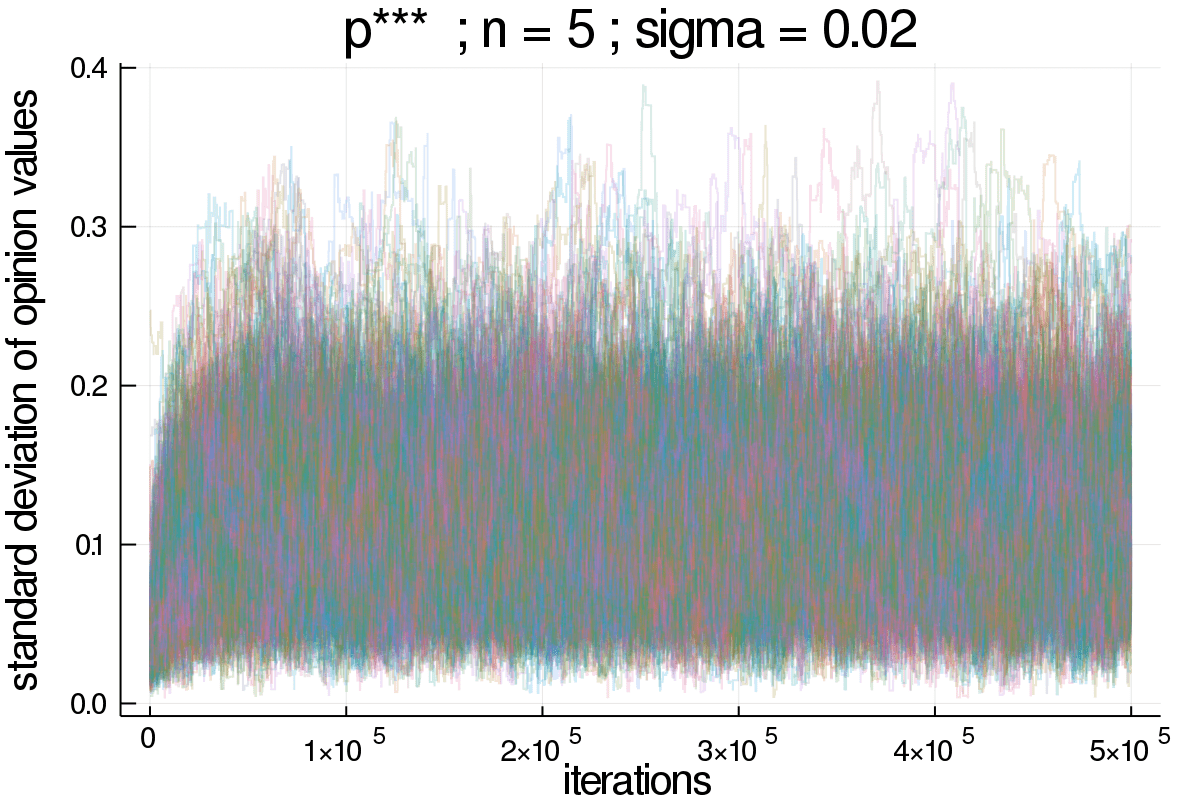
\includegraphics[width=\textwidth]{img/series/tseries2/Poodlcalculatepsssn5-rho005-sigma002-00intransrandom-std.png}
        % \caption{\textcolor{red}{'ill fix thix}}
  %    \end{subfigure}

      \begin{subfigure}[b]{0.48\textwidth}
        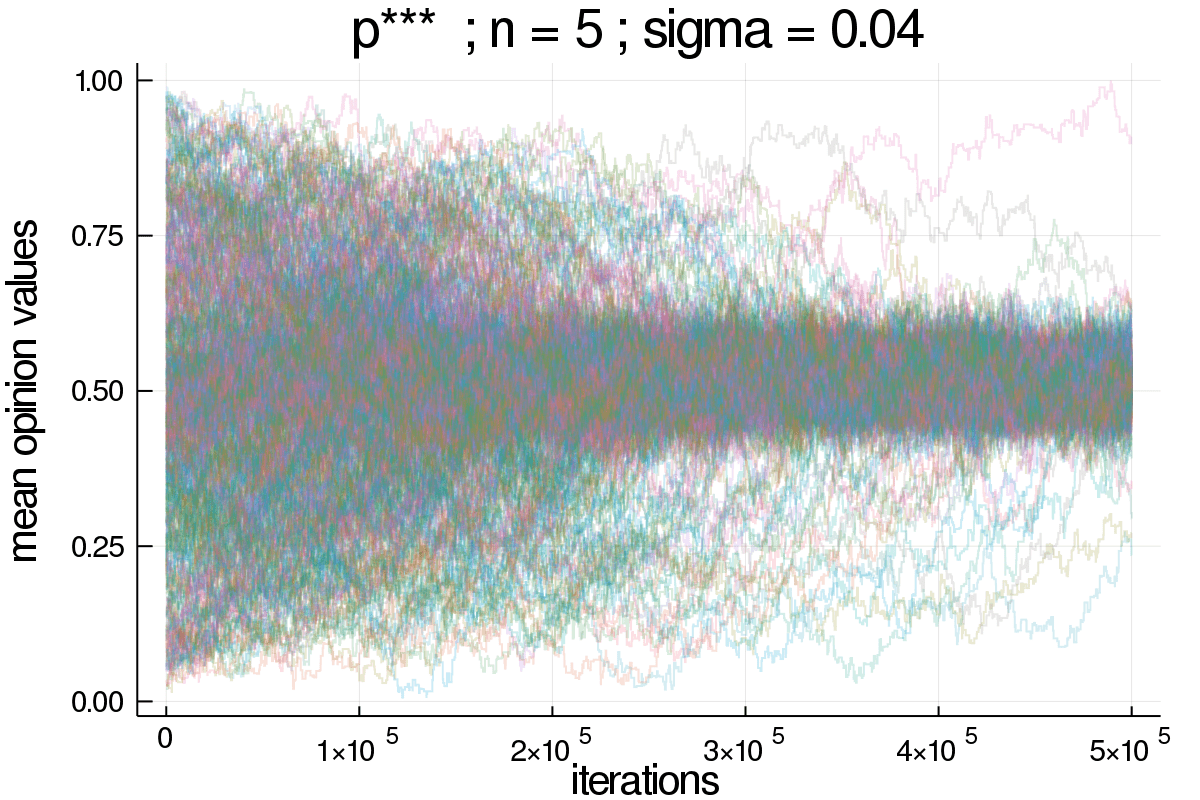
\includegraphics[width=\textwidth]{img/series/tseries2/Poodlcalculatepsssn5-rho005-sigma004-00intransrandom.png}
        % \caption{\(n\_issues = 1, \sigma = 0.02\) }
      \end{subfigure}
      % \begin{subfigure}[b]{0.48\textwidth}
      %   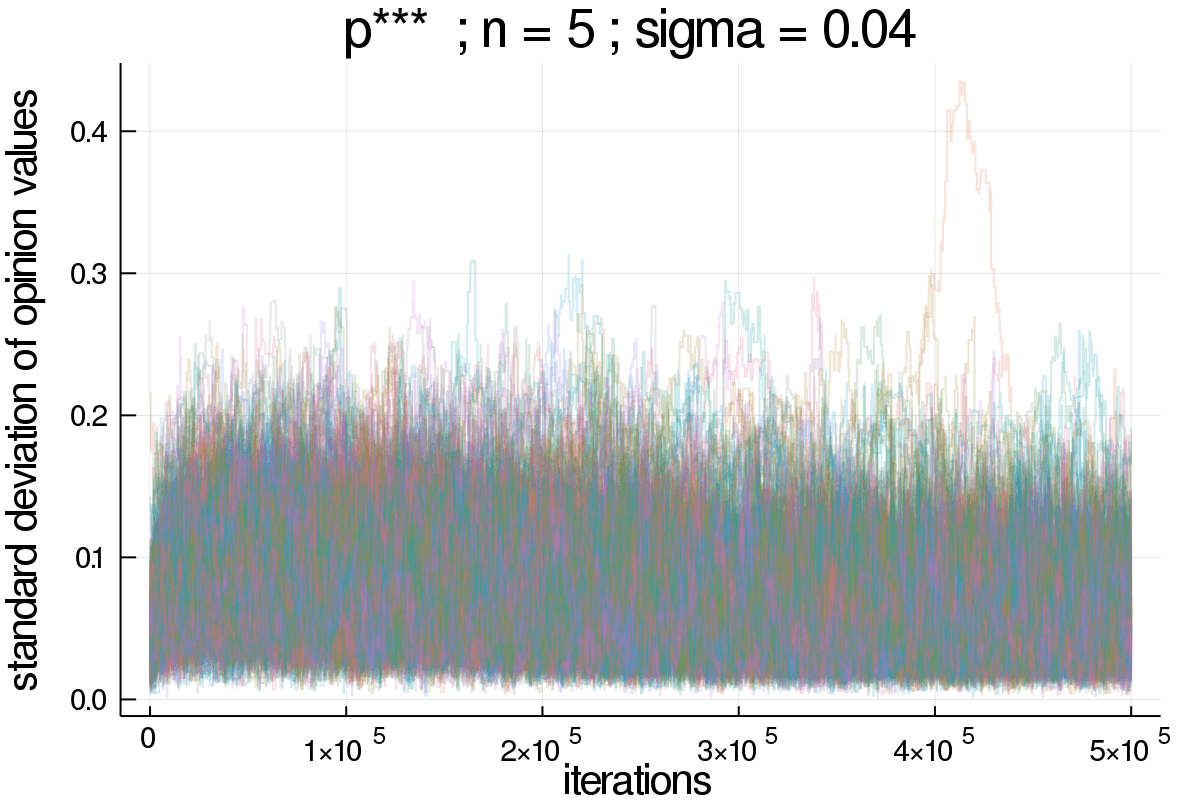
\includegraphics[width=\textwidth]{img/series/tseries2/Poodlcalculatepsssn5-rho005-sigma004-00intransrandom-std.png}
      % \end{subfigure}

      \begin{subfigure}[b]{0.48\textwidth}
        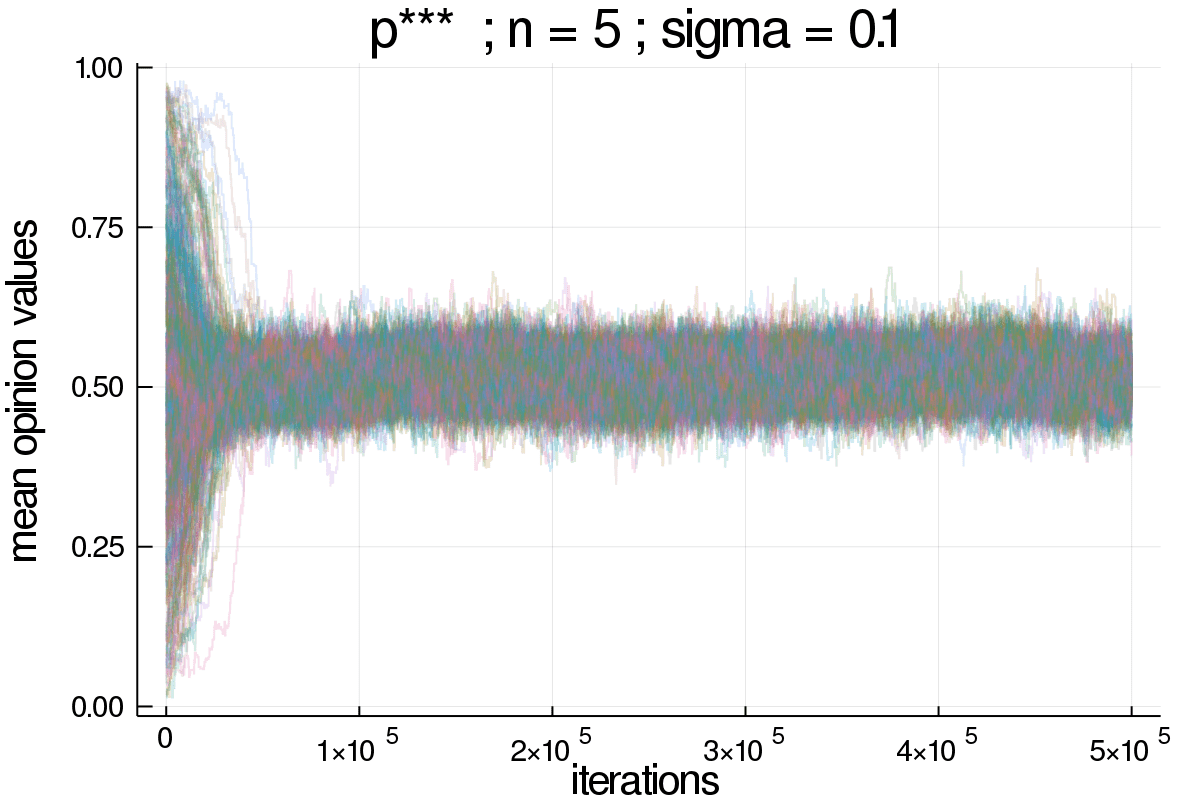
\includegraphics[width=\textwidth]{img/series/tseries2/Poodlcalculatepsssn5-rho005-sigma01-00intransrandom.png}
        % \caption{\(n\_issues = 7, \sigma = 0.1\)}
        % \caption{\(n\_issues = 1, \sigma = 0.02\) }
      \end{subfigure}
      % \begin{subfigure}[b]{0.48\textwidth}
      %   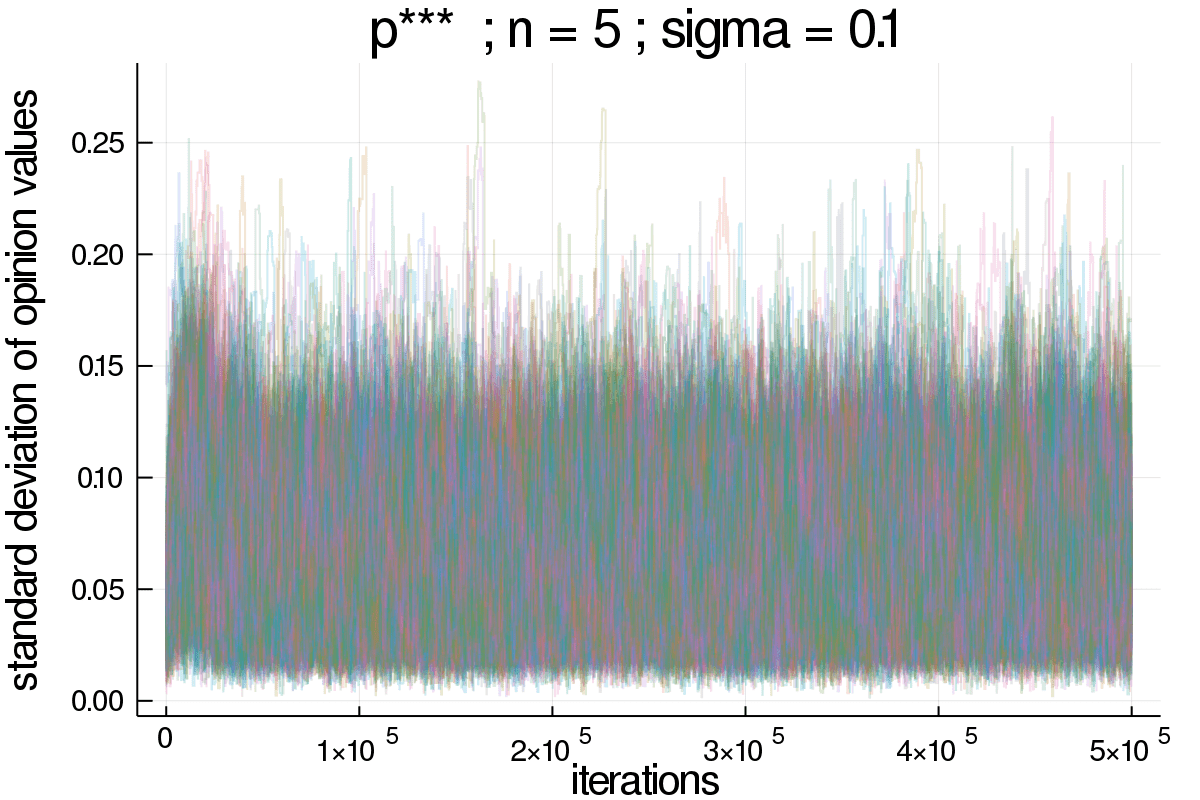
\includegraphics[width=\textwidth]{img/series/tseries2/Poodlcalculatepsssn5-rho005-sigma01-00intransrandom-std.png}
      %   % \caption{\(n\_issues = 7, \sigma = 0.1\)}
      % \end{subfigure}
      \caption{Time series for the parameterization: \(\rho = 0.05, N = 500,
        p\_intran = 0.0\)}
            \label{fig:tseries2}
          \end{figure}

          A possible reason we need to check is the fact we are measuring the
          mean opinion values \( x_i \). As \(\rho\) changes a single \(o_i\) at
          each iteration, that means a higher \(n\) should imply a lesser impact
          of \(\rho\) on the mean opinion of the agent. That could explain why,
          for a larger $n$, consensus might come easier. To test if that was
          what was actually happening, we ran the same scenarios but increasing
          \(\rho\) with \(n\), such that \(\rho_2 = \sqrt{n} * \rho_1 \). The
          effects of increasing \(\rho\) that way in the case of Figure
          \ref{fig:tseries2} can be seen at Figure \ref{fig:tseries3}. A
          comparison with Figure \ref{fig:tseries1} shows a larger spread around
          the consensus, suggesting there might be other effects here other than
          random fluctuations.


    \begin{figure}[H]
      \centering
      \begin{subfigure}[b]{0.48\textwidth}
      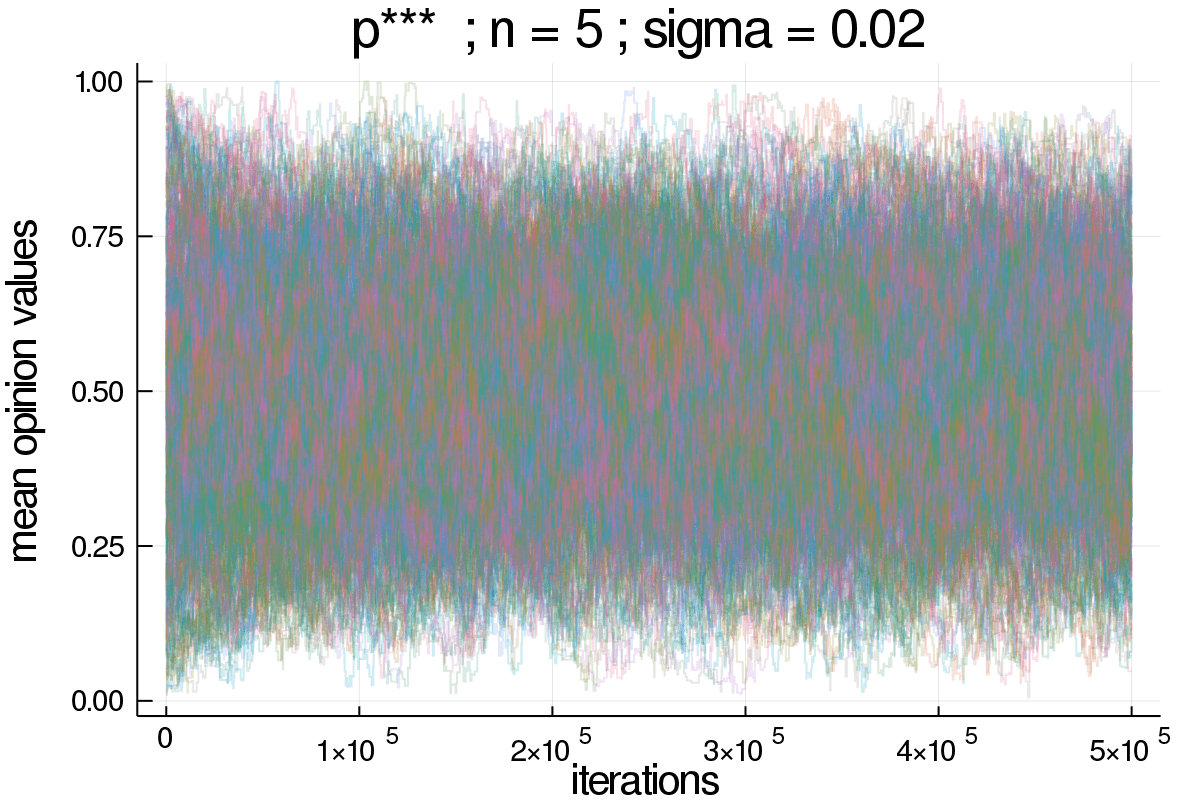
\includegraphics[width=0.9\textwidth]{img/series/tseries3/Poodlcalculatepsssn5-rho01118033988749895-sigma002-00intransrandom.png}
    \end{subfigure}
    %       \begin{subfigure}[b]{0.48\textwidth}
    %   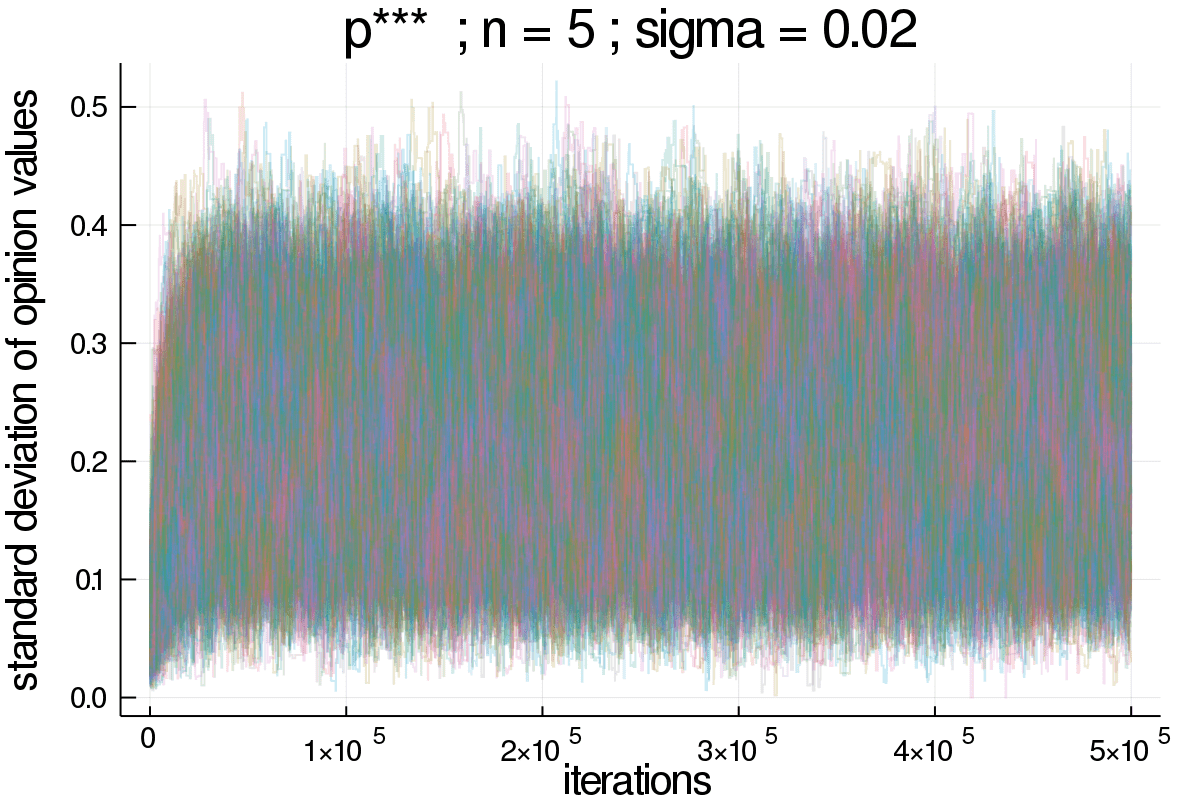
\includegraphics[width=0.9\textwidth]{img/series/tseries3/Poodlcalculatepsssn5-rho01118033988749895-sigma002-00intransrandom-std.png}
    % \end{subfigure}
    \begin{subfigure}[b]{0.48\textwidth}
      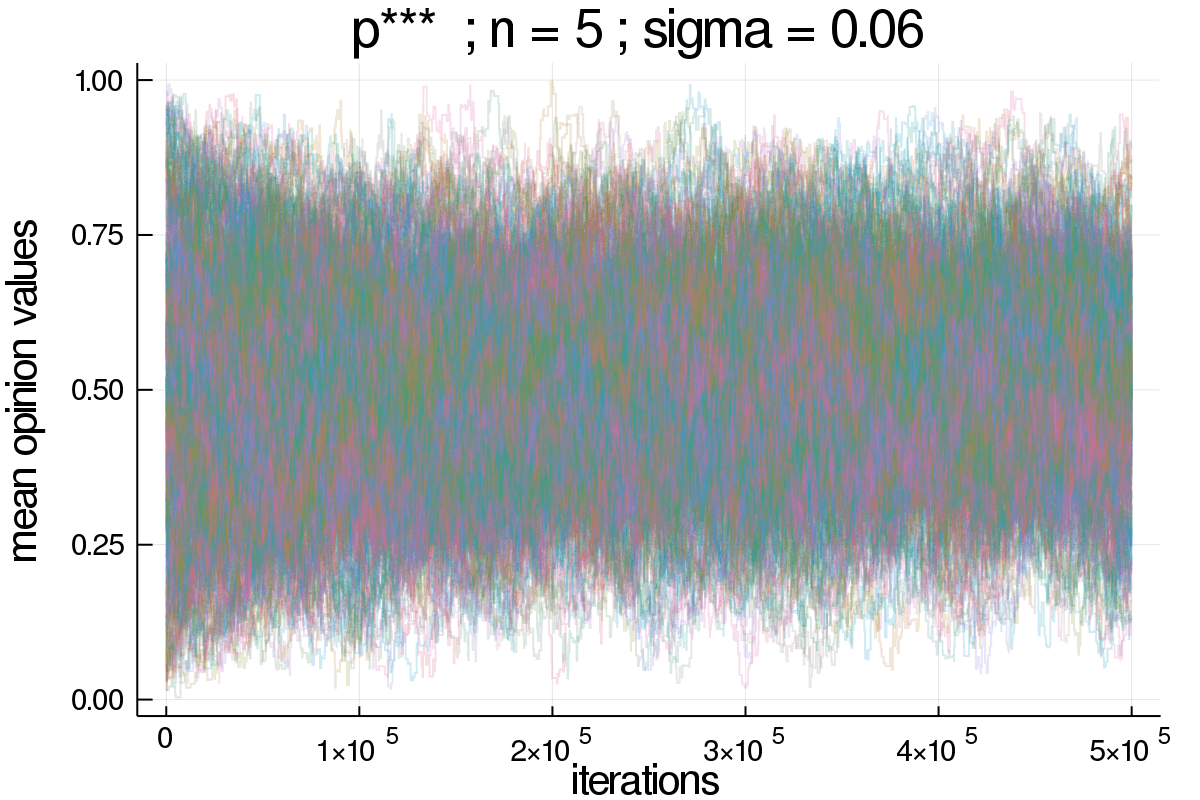
\includegraphics[width=0.9\textwidth]{img/series/tseries3/Poodlcalculatepsssn5-rho01118033988749895-sigma006-00intransrandom.png}
    \end{subfigure}
    % \begin{subfigure}[b]{0.48\textwidth}
    %   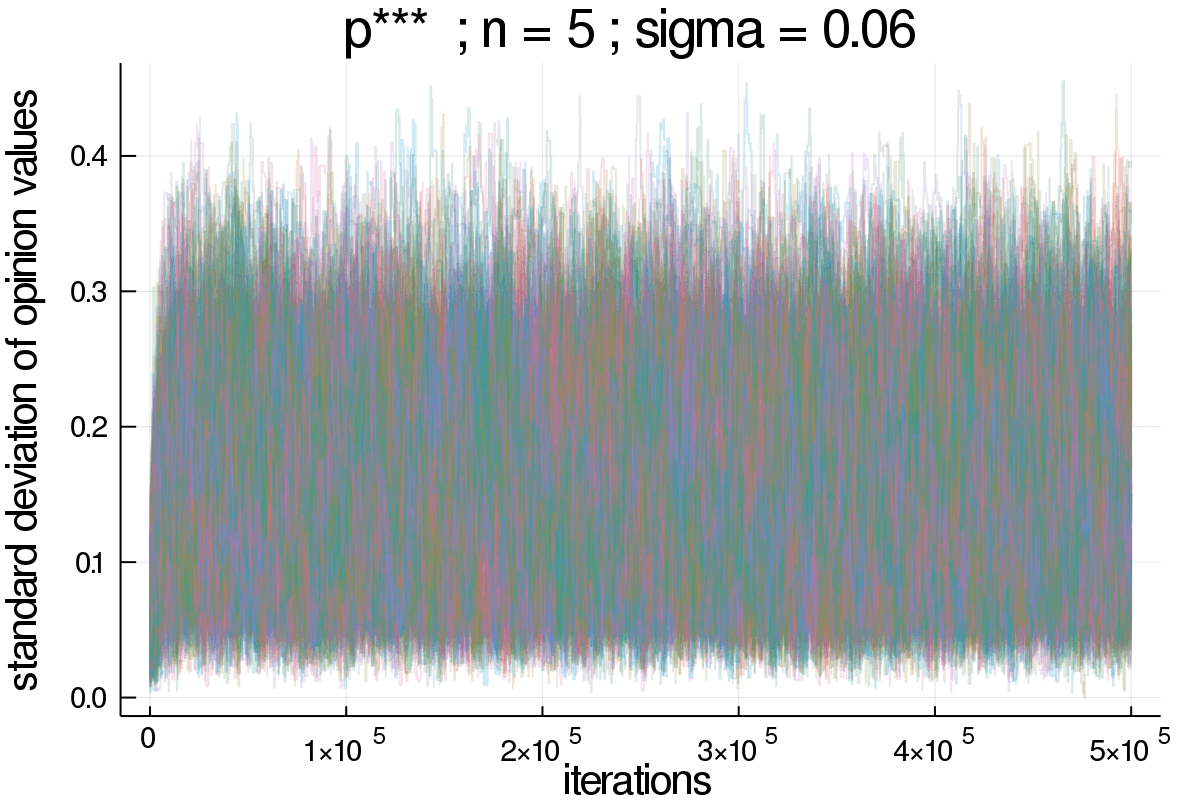
\includegraphics[width=0.9\textwidth]{img/series/tseries3/Poodlcalculatepsssn5-rho01118033988749895-sigma006-00intransrandom-std.png}
    % \end{subfigure}
      \begin{subfigure}[b]{0.48\textwidth}
      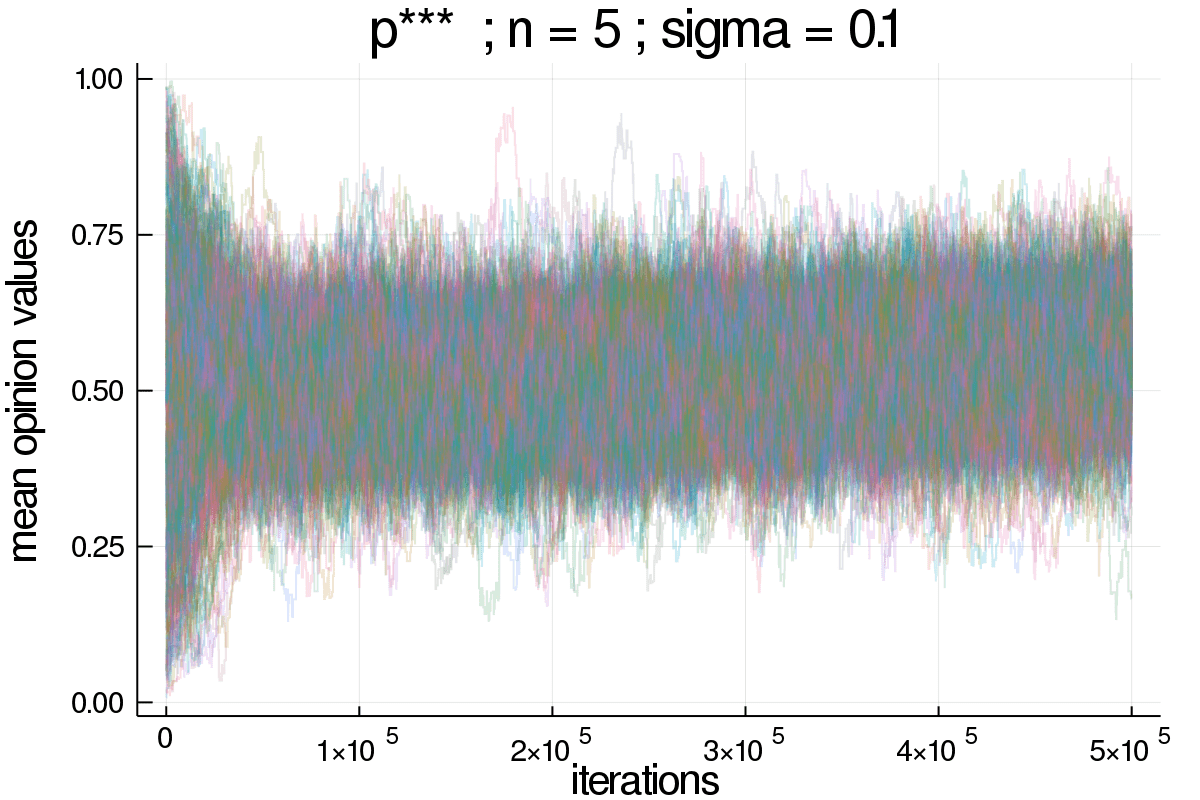
\includegraphics[width=0.9\textwidth]{img/series/tseries3/Poodlcalculatepsssn5-rho01118033988749895-sigma01-00intransrandom.png}
    \end{subfigure}
  % \begin{subfigure}[b]{0.48\textwidth}
  %     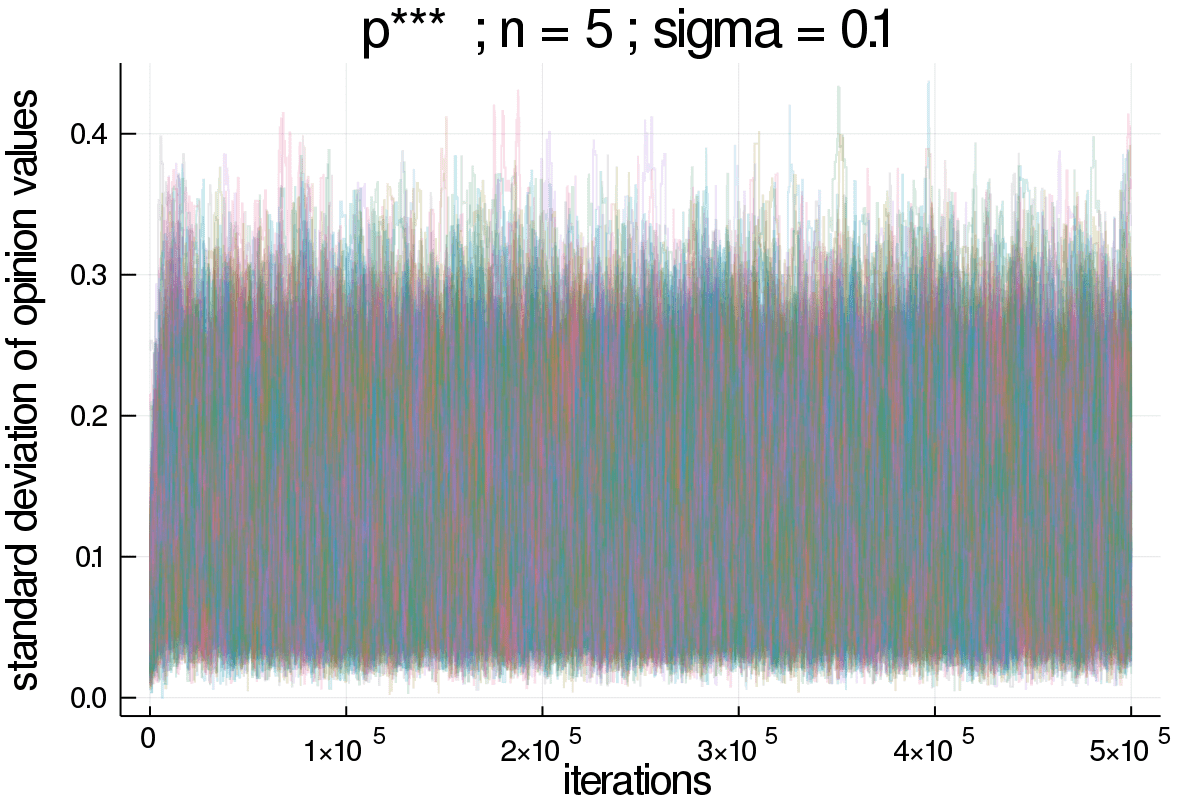
\includegraphics[width=0.9\textwidth]{img/series/tseries3/Poodlcalculatepsssn5-rho01118033988749895-sigma01-00intransrandom-std.png}
  %     \end{subfigure}

      \caption{Time series for the parameterization: \(\rho \approx 0.12, N =
        500, p\_intran = 0.0 \)}
      \label{fig:tseries3}
    \end{figure}

    Heretofore we've tested parameterizations with noise. To verify the
    influence of the existence of noise, we also ran cases with \(\rho\) close to
    zero,that is \(\rho = 10^{-5} \). The most obvious difference we can see is
    that the population mean opinion values converge to well defined values. In
    parameter combinations in which \(\sigma = 0.1\) the tendency is convergence
    to values close to 0.5. An interesting distinction between the cases in this
    parameterization is that \(p^{**}\) and \(p^{***}\) always converge to 0.5,
    independently of the number of issues. Alternatively, in the \(p^{*}\) case
    this happens when \(n=1\), but when we have \(n=5\) or \(10\) there are
    other values of convergence, more as we increase \(n\), even though the
    centralizing tendency remains.
    \begin{figure}[H]
      \centering
      \begin{subfigure}[b]{0.48\textwidth}
        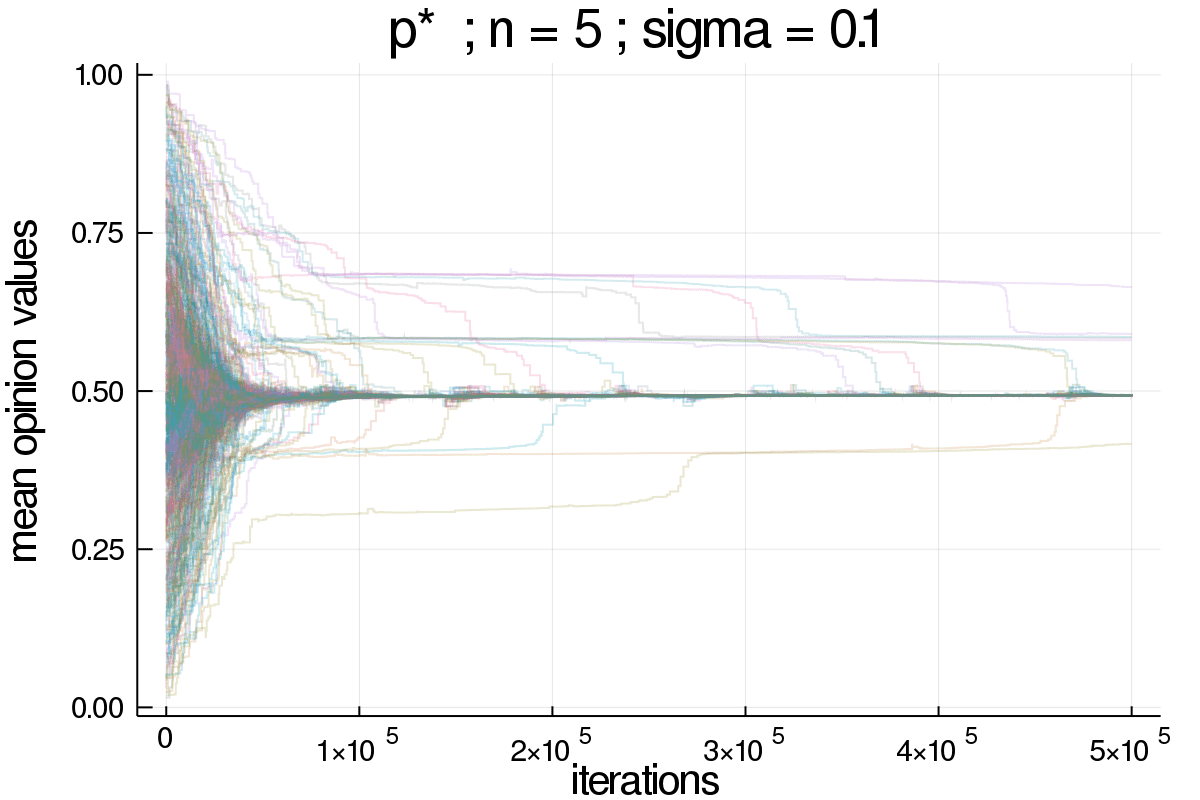
\includegraphics[width=\textwidth]{img/series/tseries4/Poodlcalculatepsn5-rho10e-5-sigma01-00intransrandom.png}
        % \caption{\textcolor{red}{'ill fix thix}}
      \end{subfigure}
      % \begin{subfigure}[b]{0.48\textwidth}
      %   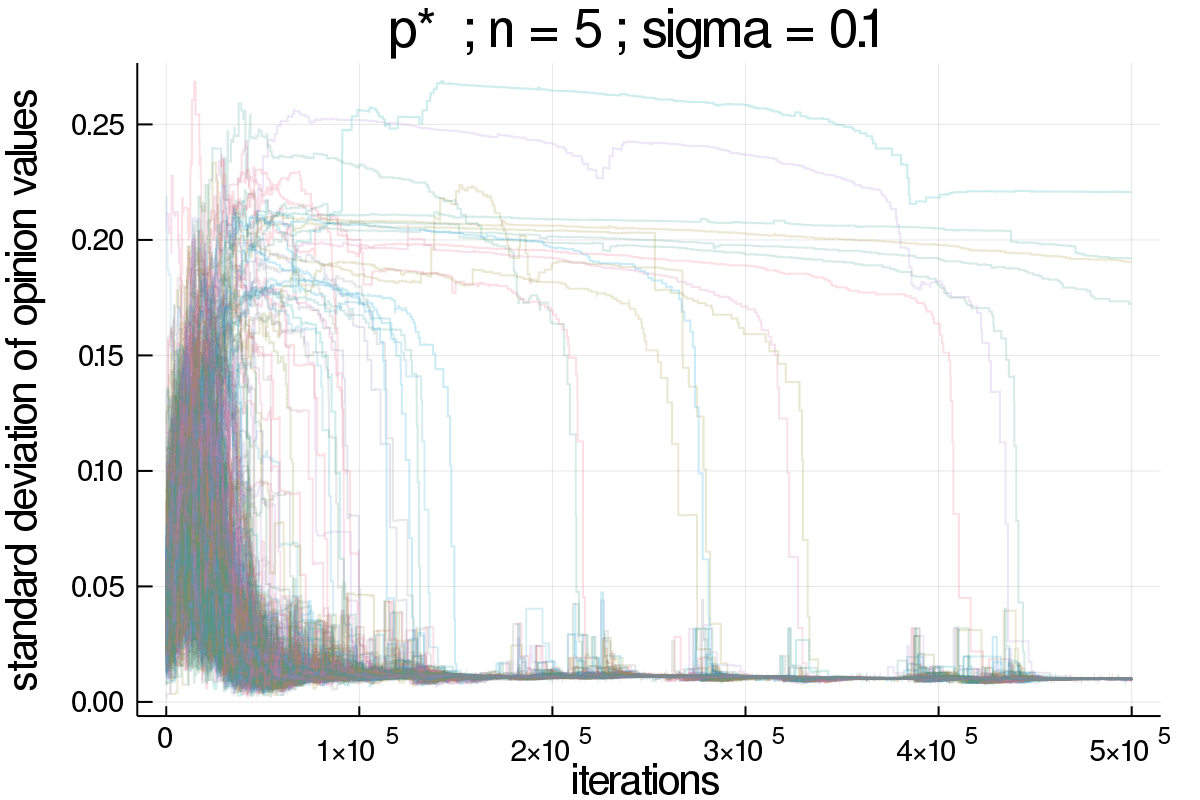
\includegraphics[width=\textwidth]{img/series/tseries4/Poodlcalculatepsn5-rho10e-5-sigma01-00intransrandom-std.png}
      %   % \caption{\textcolor{red}{'ill fix thix}}
      % \end{subfigure}
      \begin{subfigure}[b]{0.48\textwidth}
        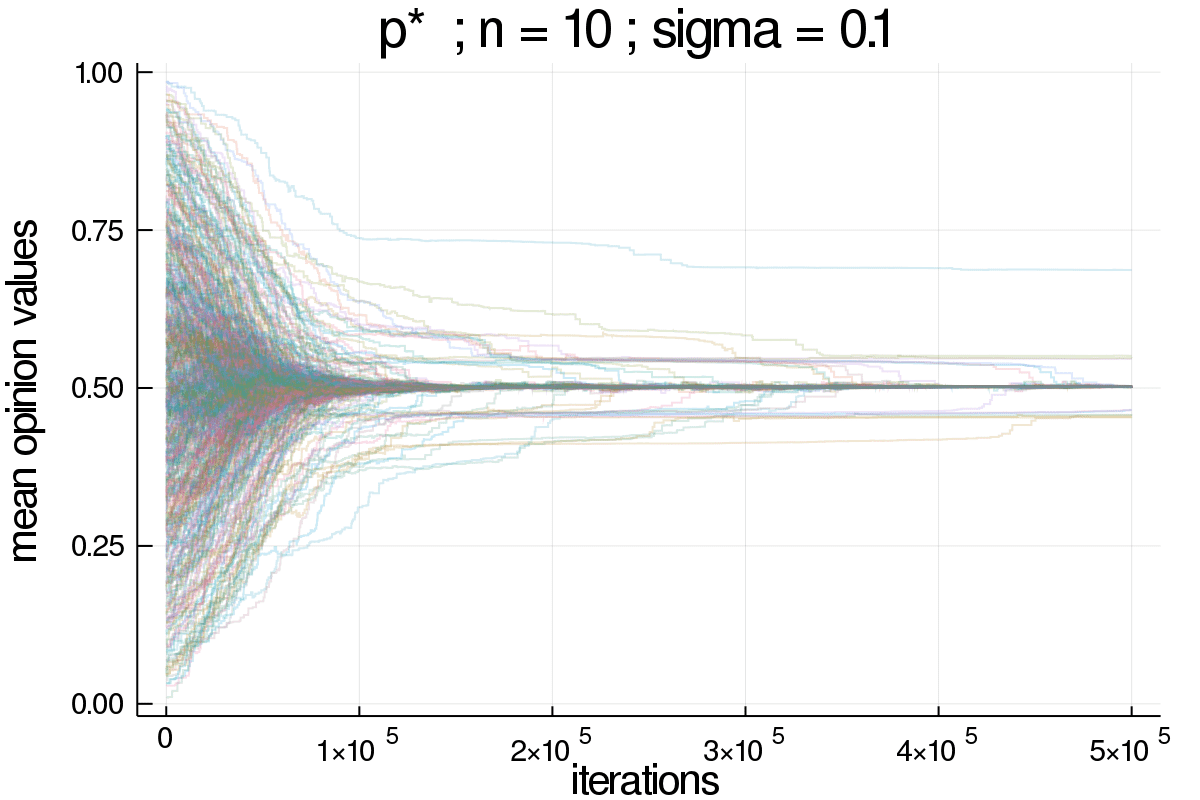
\includegraphics[width=\textwidth]{img/series/tseries4/Poodlcalculatepsn10-rho10e-5-sigma01-00intransrandom.png}
        % \caption{\(n\_issues = 1, \sigma = 0.02\) }
      \end{subfigure}
      % \begin{subfigure}[b]{0.48\textwidth}
      %   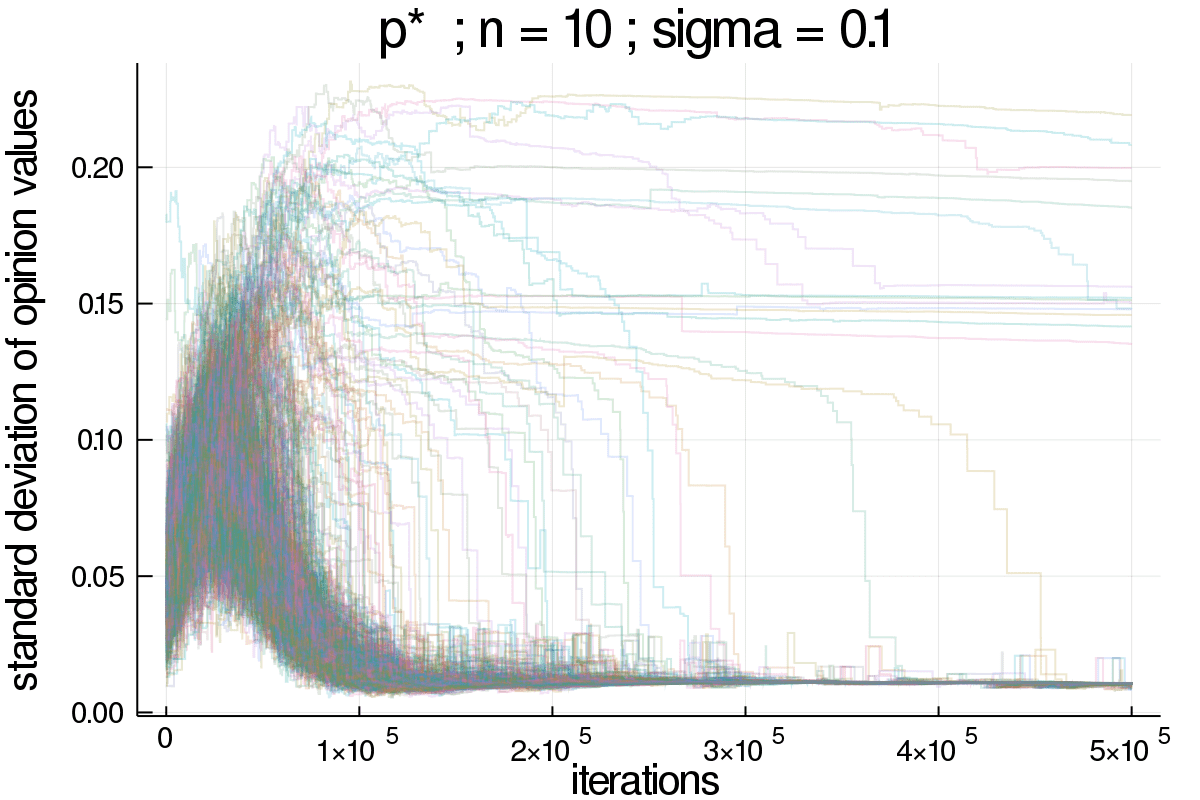
\includegraphics[width=\textwidth]{img/series/tseries4/Poodlcalculatepsn10-rho10e-5-sigma01-00intransrandom-std.png}
      %   % \caption{\(n\_issues = 1, \sigma = 0.02\) }
      % \end{subfigure}
      \begin{subfigure}[b]{0.48\textwidth}
        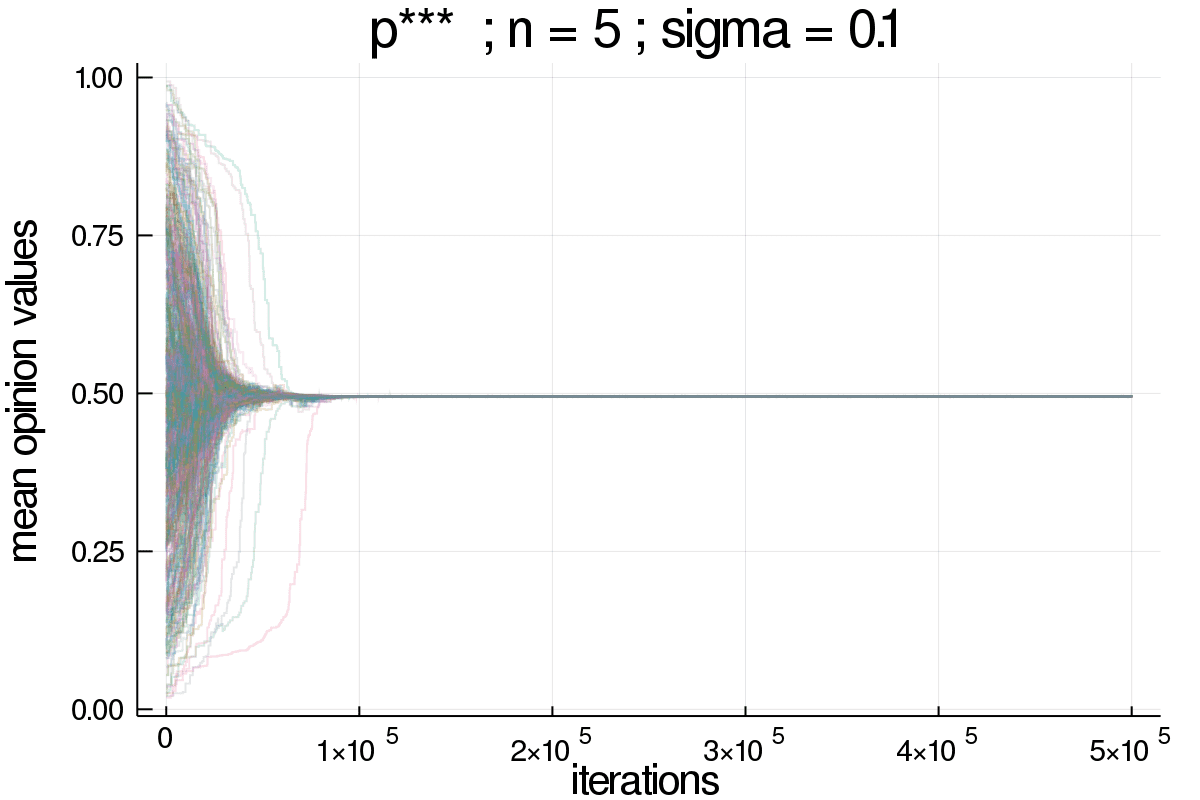
\includegraphics[width=\textwidth]{img/series/tseries4/Poodlcalculatepsssn5-rho10e-5-sigma01-00intransrandom.png}
        % \caption{\(n\_issues = 7, \sigma = 0.1\)}
      \end{subfigure}
      % \begin{subfigure}[b]{0.48\textwidth}
      %   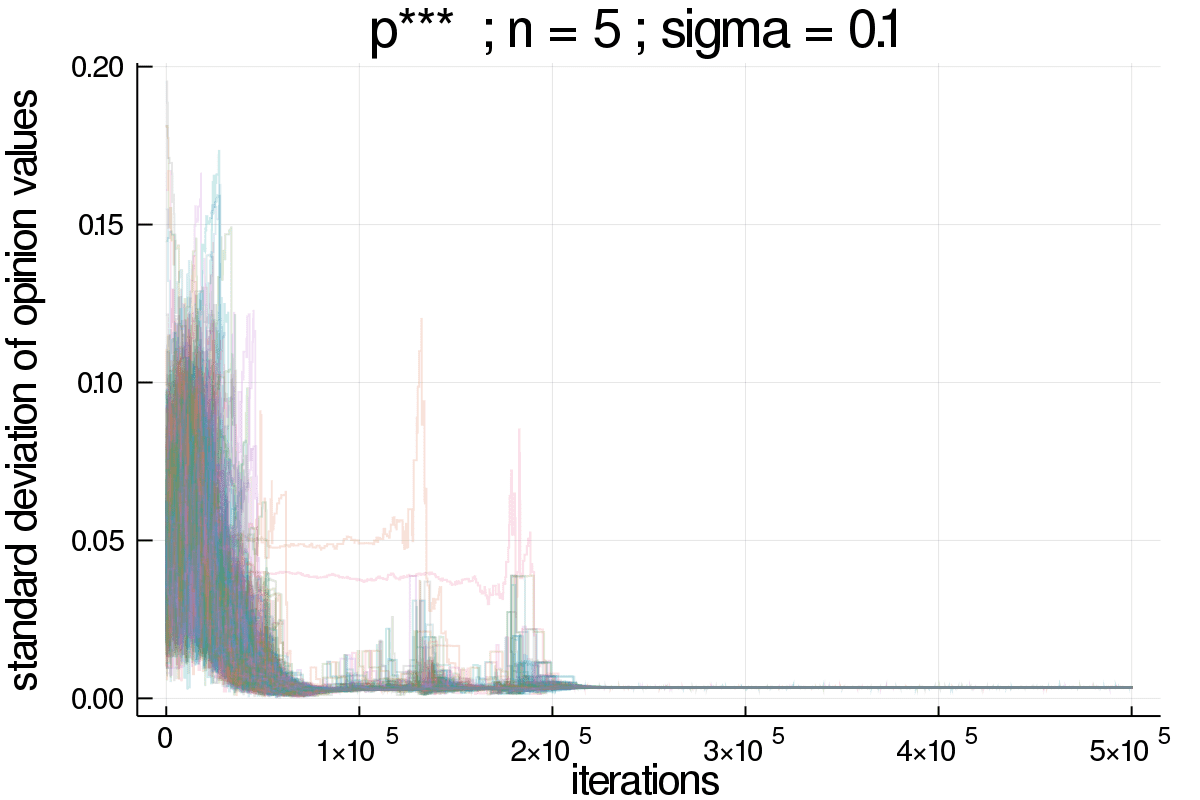
\includegraphics[width=\textwidth]{img/series/tseries4/Poodlcalculatepsssn5-rho10e-5-sigma01-00intransrandom-std.png}
      %   % \caption{\(n\_issues = 7, \sigma = 0.1\)}
      % \end{subfigure}
            \begin{subfigure}[b]{0.48\textwidth}
        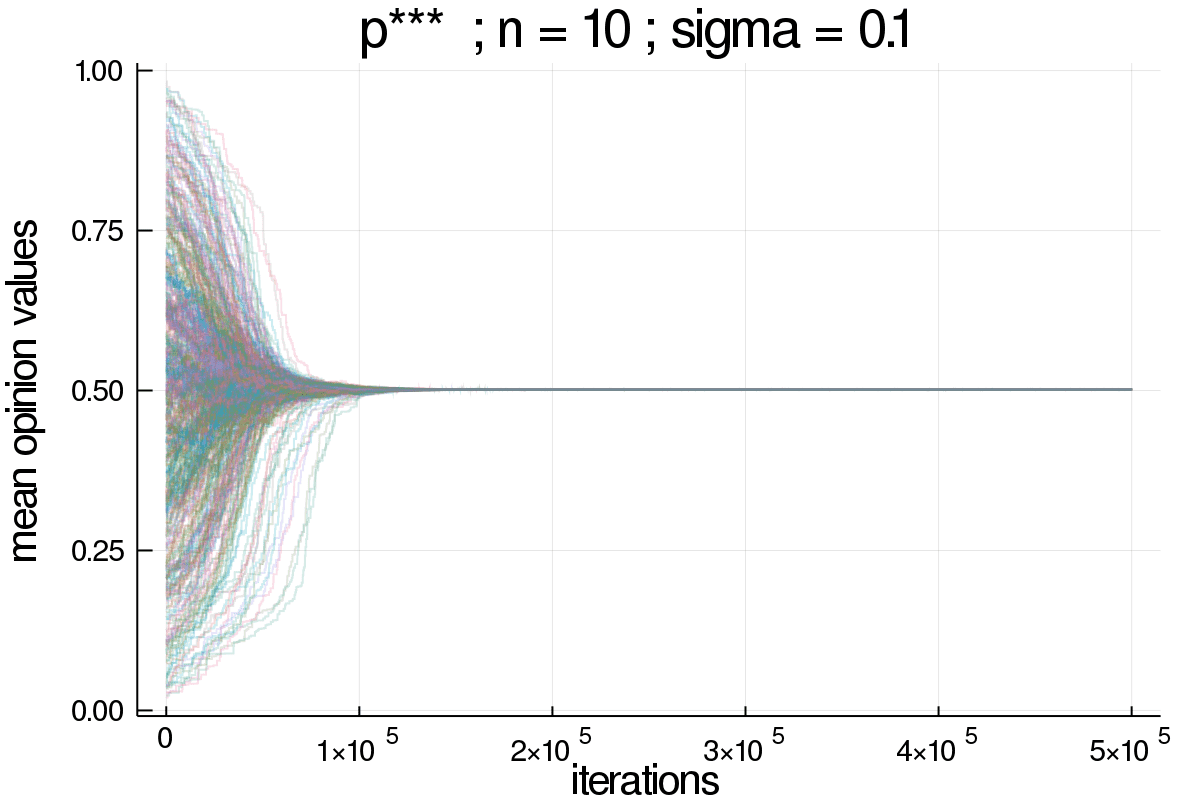
\includegraphics[width=\textwidth]{img/series/tseries4/Poodlcalculatepsssn10-rho10e-5-sigma01-00intransrandom.png}
        % \caption{\(n\_issues = 7, \sigma = 0.1\)}
      \end{subfigure}
      % \begin{subfigure}[b]{0.48\textwidth}
      %   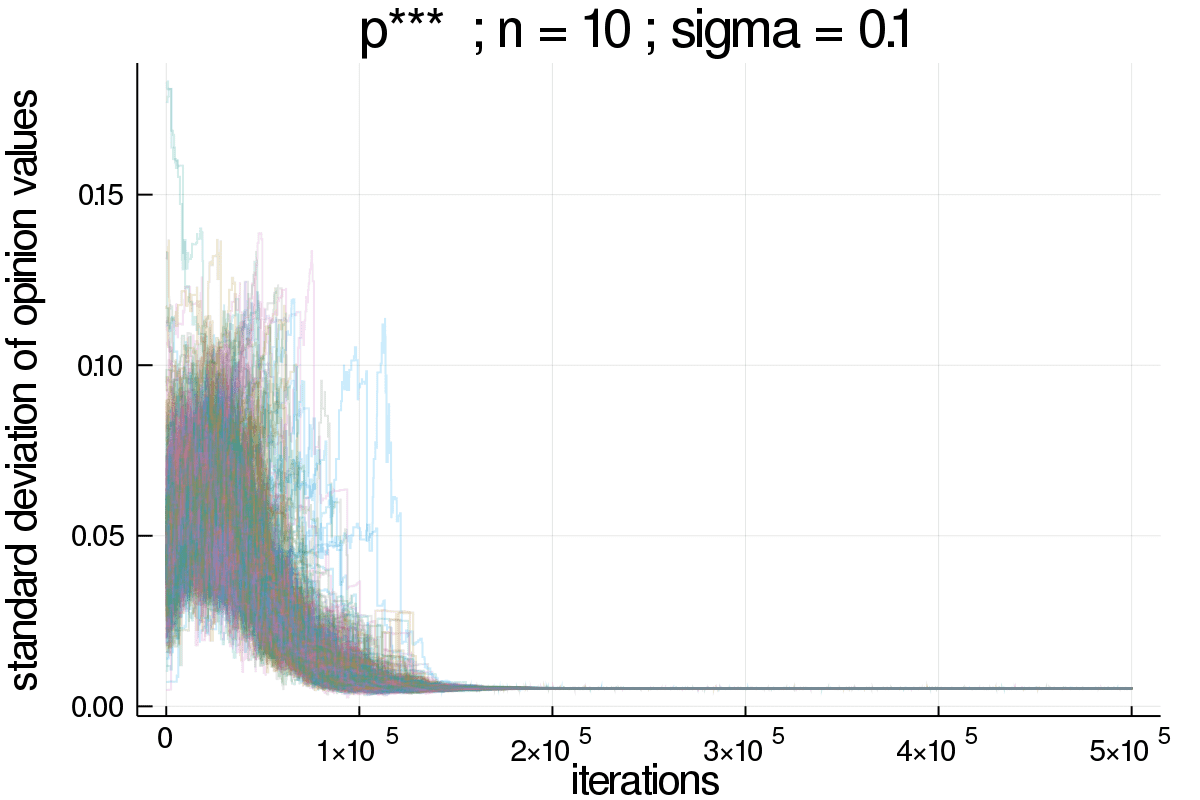
\includegraphics[width=\textwidth]{img/series/tseries4/Poodlcalculatepsssn10-rho10e-5-sigma01-00intransrandom-std.png}
      %   % \caption{\(n\_issues = 7, \sigma = 0.1\)}
      % \end{subfigure}
      \caption{Time series for the parameterization: \(\rho = 1e-5, N =
        500, p\_intran = 0.0 \)}
      \label{fig:tseries4}
    \end{figure}

    When \(\sigma\) is around \(0.02\) or \(0.04\), we observe another
    difference between cases: \(p^{*}\) has more convergence values than
    \(p^{**}\) and \(p^{***}\). Figure \ref{fig:tseries5} illustrates this
    system behavior for $\sigma=0.02$. We can also see that the standard
    deviations $s_i$ are very different for the \(p^{*}\) and \(p^{***}\) cases.
    While for \(p^{*}\), the values of $s_i$ range from small values around 0.02
    to much larger values, up tp 0.2, in the \(p^{***}\) scenario we see that
    $s_i$ tends to diminish with time, the majority of the observed values
    getting close to zero.

    \begin{figure}[H]
      \centering
      \begin{subfigure}[b]{0.48\textwidth}
        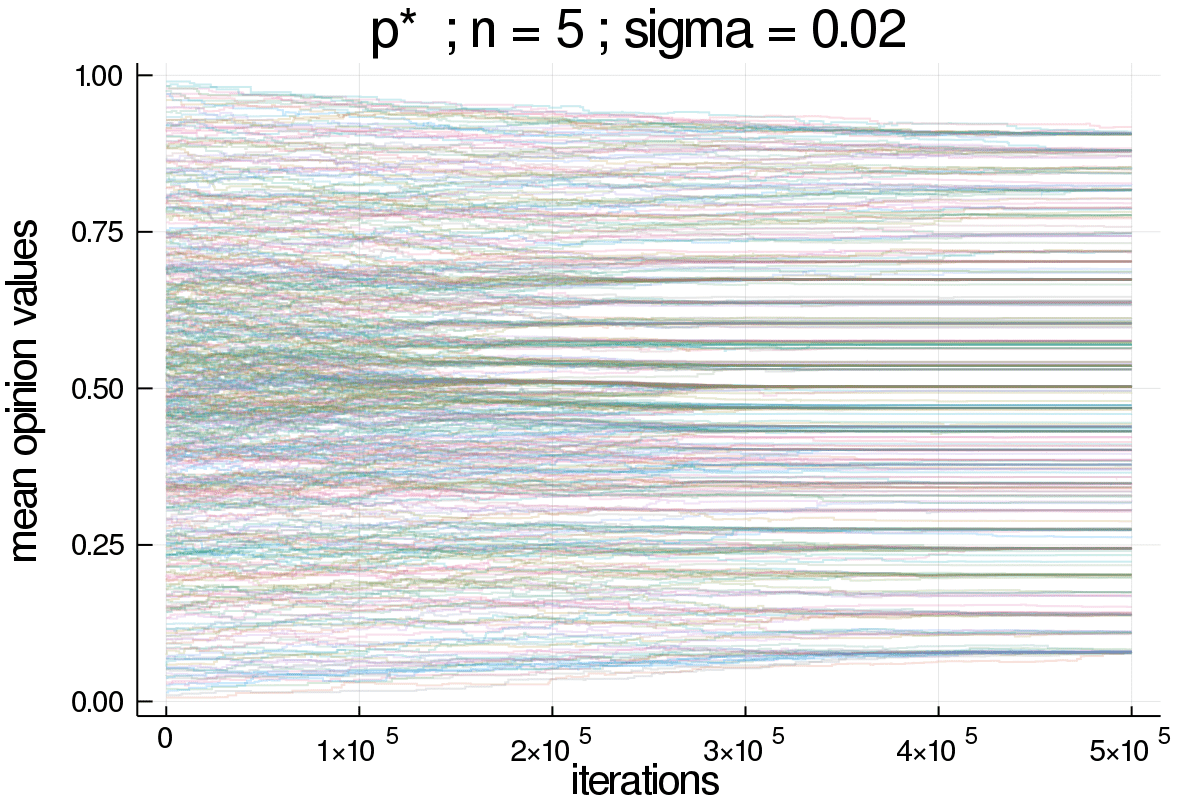
\includegraphics[width=\textwidth]{img/series/tseries5/Poodlcalculatepsn5-rho10e-5-sigma002-00intransrandom.png}
        % \caption{\textcolor{red}{'ill fix thix}}
      \end{subfigure}
      \begin{subfigure}[b]{0.48\textwidth}
        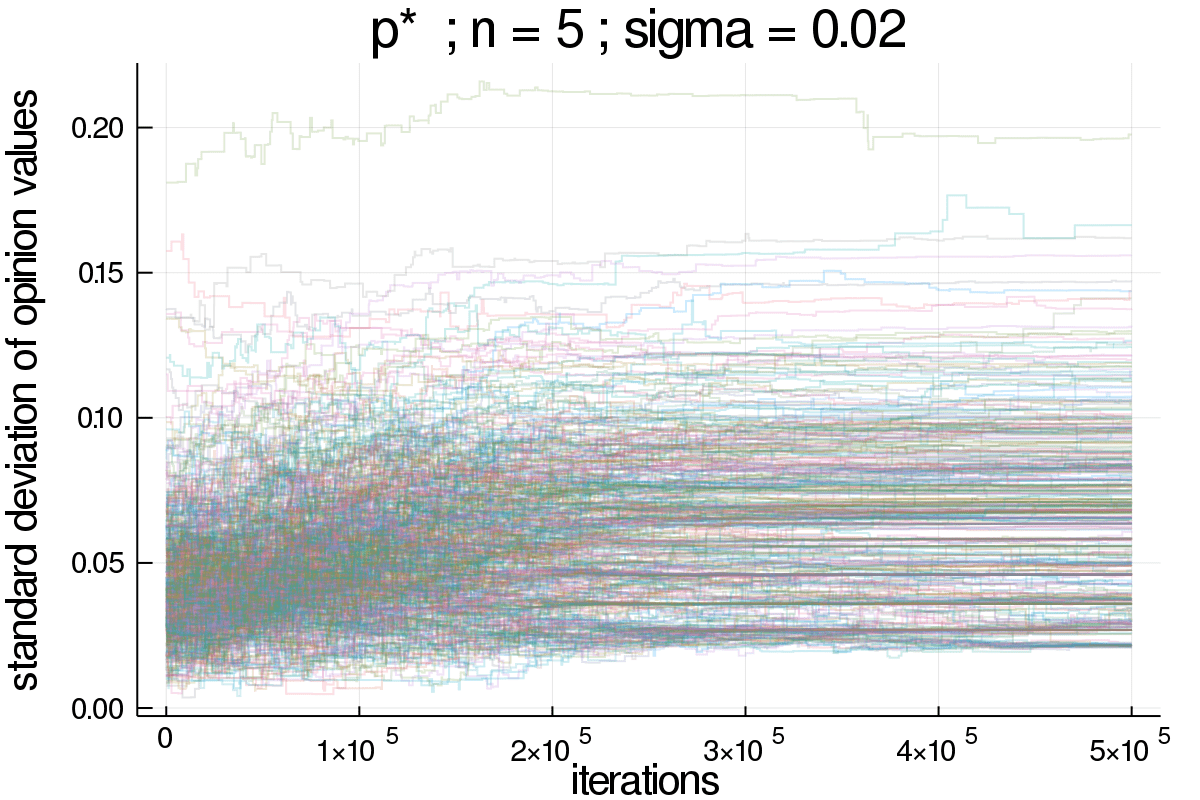
\includegraphics[width=\textwidth]{img/series/tseries5/Poodlcalculatepsn5-rho10e-5-sigma002-00intransrandom-std.png}
        % \caption{\textcolor{red}{'ill fix thix}}
        \end{subfigure}
      \begin{subfigure}[b]{0.48\textwidth}
        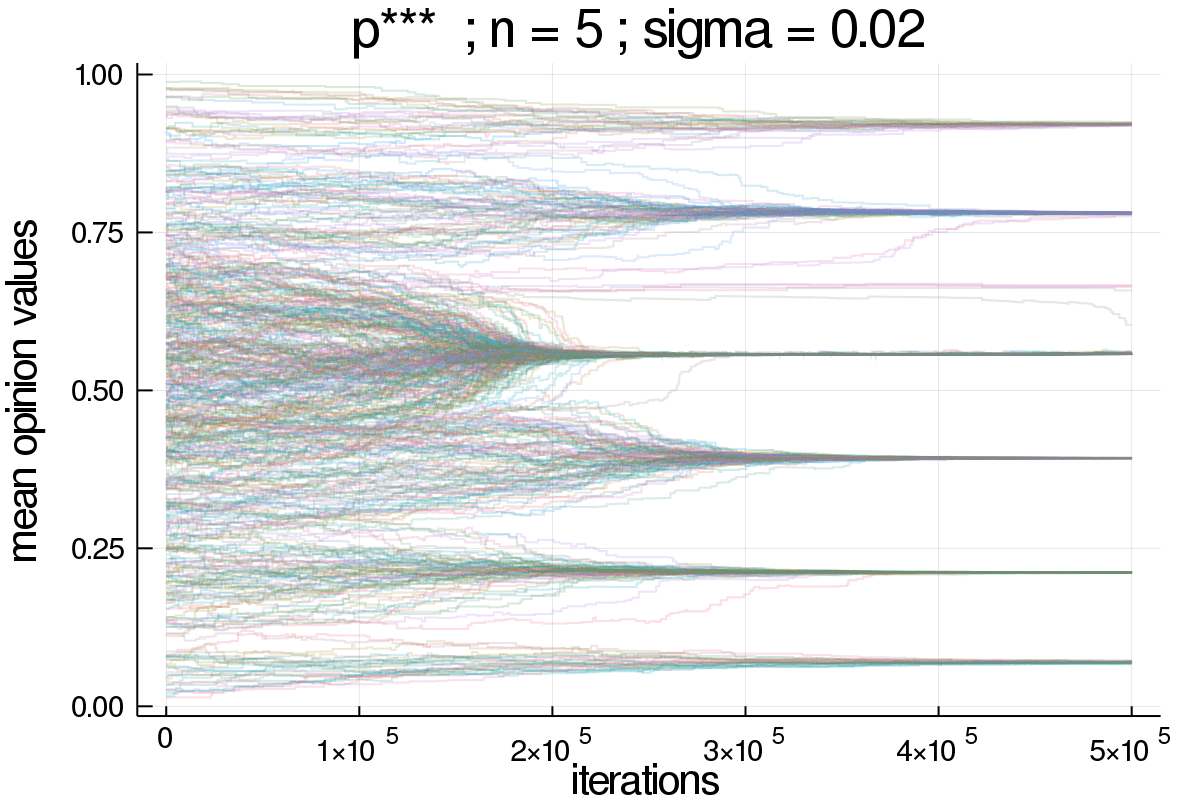
\includegraphics[width=\textwidth]{img/series/tseries5/Poodlcalculatepsssn5-rho10e-5-sigma002-00intransrandom.png}
        % \caption{\(n\_issues = 1, \sigma = 0.02\) }
      \end{subfigure}
      \begin{subfigure}[b]{0.48\textwidth}
        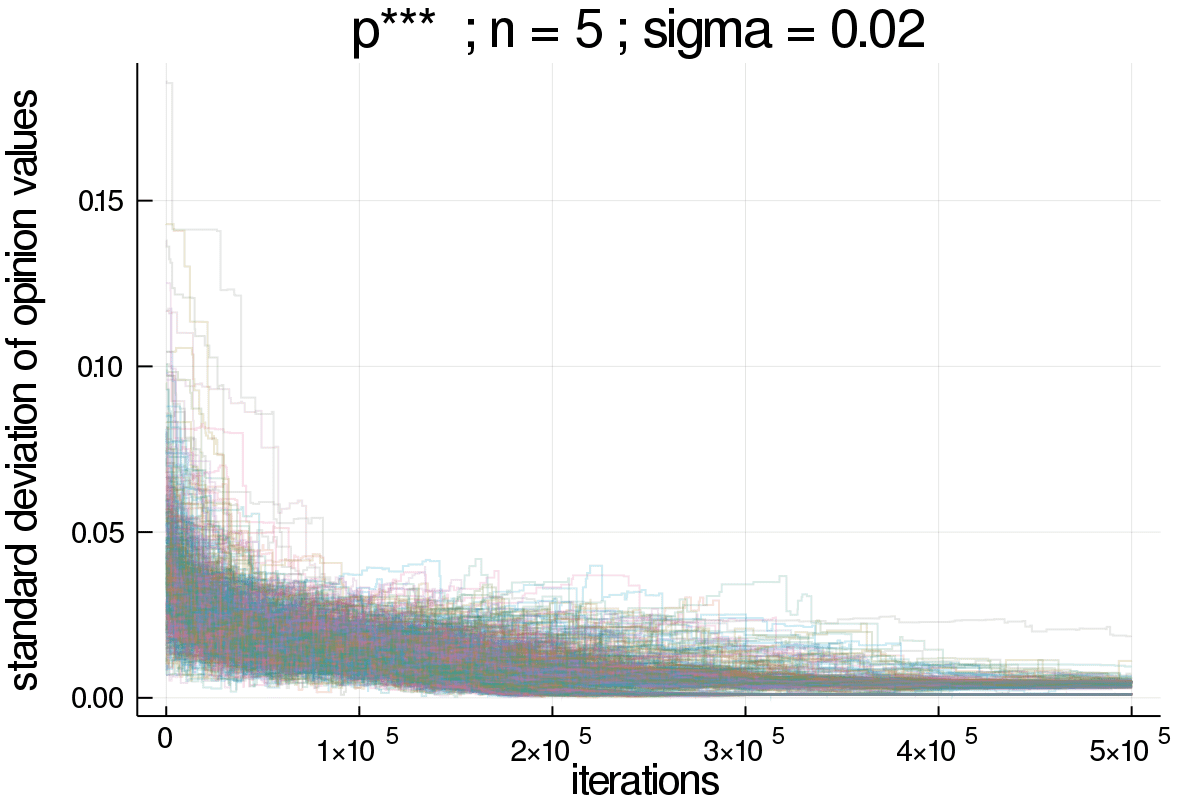
\includegraphics[width=\textwidth]{img/series/tseries5/Poodlcalculatepsssn5-rho10e-5-sigma002-00intransrandom-std.png}
        % \caption{\(n\_issues = 1, \sigma = 0.02\) }
      \end{subfigure}
      \caption{Time series for the parameterization: \(\rho = 1e-5, N =
        500, p\_intran = 0.0 \)}
  \label{fig:tseries5}
    \end{figure}

    The reason for that lies in how \(\Delta\) (that controls how much an agent
    will trust others) is calculated in each case: in the \(p^{**}\) and
    \(p^{***}\) cases the update rules make use of mean opinion values. That
    introduces a tendency for distinct issues opinions to move towards each
    other. The \(p^{*}\) update rule, however, works with single issue opinions.
    As the issues are uncoupled, that allows the agents to keep an ideologically
    more diverse profile.

    Another impact of the number of issues, as shown in Figure
    \ref{fig:tseries6}, is that a higher \(n\) leads to a longer time for the
    convergence. The reason is that we're only changing one
    opinion by iteration, so naturally a higher \(n\) means the agents will take
    longer to be influenced. The relationship here is roughly linear such that
    the plot the region at \(5 \times 10^5\) iterations when \(n = 10\) is very
    similar to the corresponding region at \(0.5 \times 10^5\) when \(n = 1\).

    \begin{figure}[H]
      \centering

      \begin{subfigure}[b]{0.49\textwidth}
        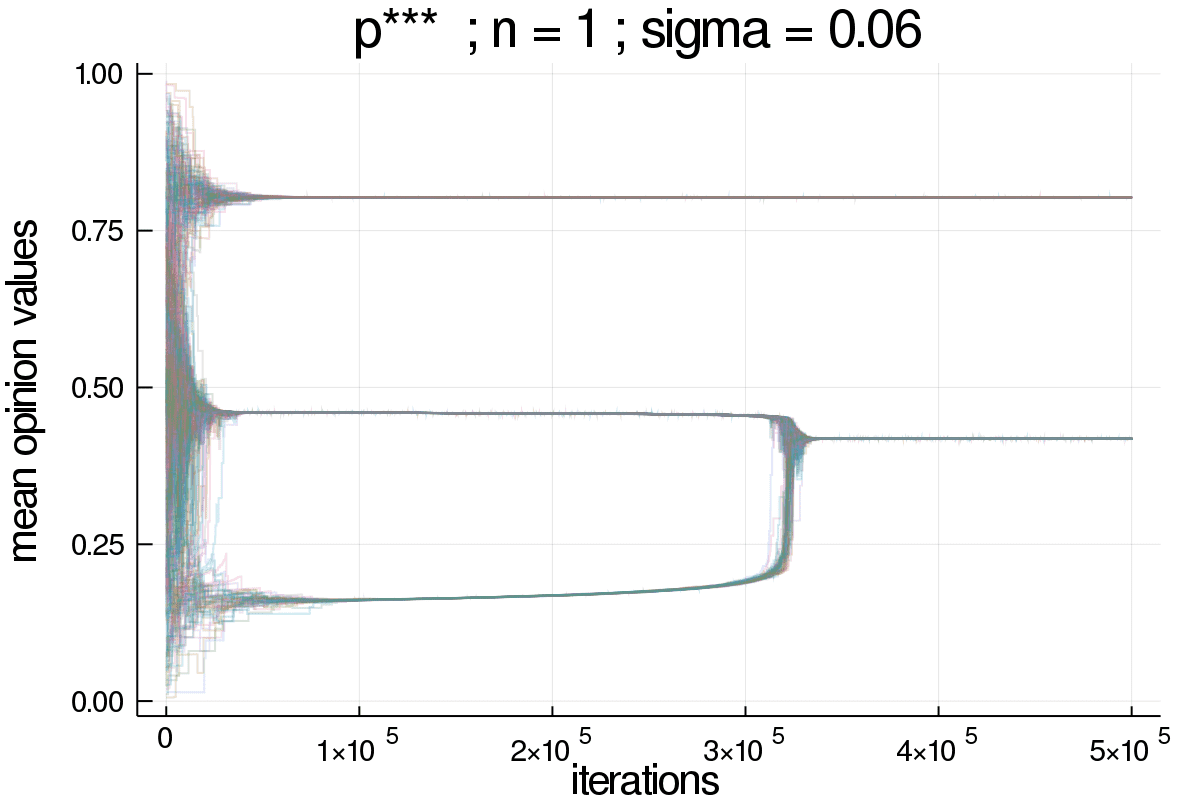
\includegraphics[width=\textwidth]{img/series/tseries6/Poodlcalculatepsssn1-rho10e-5-sigma006-00intransrandom.png}
        % \caption{\textcolor{red}{'ill fix thix}}
      \end{subfigure}

      \begin{subfigure}[b]{0.49\textwidth}
        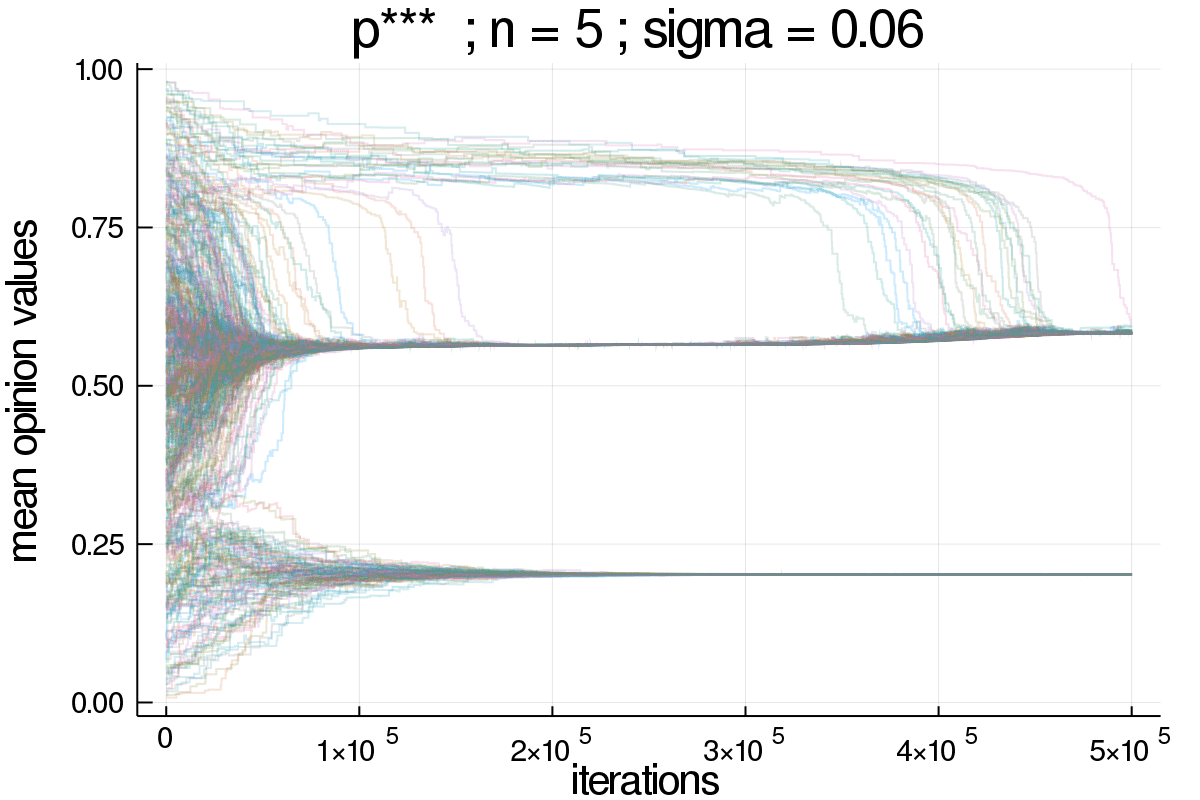
\includegraphics[width=\textwidth]{img/series/tseries6/Poodlcalculatepsssn5-rho10e-5-sigma006-00intransrandom.png}
        % \caption{\(n\_issues = 1, \sigma = 0.02\) }
      \end{subfigure}
      % \begin{subfigure}[b]{0.49\textwidth}
      %   \includegraphics[width=\textwidth]{img/series/tseries6/Poodlcalculatepsssn5-rho10e-5-sigma006-00intransrandom-std.png}
      %   % \caption{\(n\_issues = 1, \sigma = 0.02\) }
      % \end{subfigure}
            \begin{subfigure}[b]{0.49\textwidth}
        \includegraphics[width=\textwidth]{img/series/tseries6/Poodlcalculatepsssn10-rho10e-5-sigma006-00intransrandom.png}
        % \caption{\(n\_issues = 1, \sigma = 0.02\) }
      \end{subfigure}
      % \begin{subfigure}[b]{0.49\textwidth}
      %   \includegraphics[width=\textwidth]{img/series/tseries6/Poodlcalculatepsssn10-rho10e-5-sigma006-00intransrandom-std.png}
      %   % \caption{\(n\_issues = 1, \sigma = 0.02\) }
      % \end{subfigure}
      \caption{Time series for the parameterization: \(\rho = 1e-5, N = 500,
        p\_intran = 0.0 \).}
  \label{fig:tseries6}
    \end{figure}

    \section{Conclusions}

    Here, we have extended a previous model for continuous opinions
    \cite{martins08c} to include the case where agents have opinions on $n$
    issues. We explored the impact of the main parameters on the final results.
    The \(\sigma\) parameter, that determines how certain each agent is of his
    opinion, was observed to be a major influence in the outcome of the
    simulations and, therefore, plays the same qualitative role in the system
    dynamics that threshold values plays in Bounded Confidence models.
    Differently from Bounded Confidence models, the global sensitivity analysis
    shows that in our model its opinion certainty, and not trust, that is the
    main driver of the dynamics\footnote{However, the trust functions also
      matter as recapitulated below.}. The number of issues $n$ as well as the
    amount of noise $\rho$ were also shown by our sensitivity analysis to have
    important effects on the outcomes, while the initial general amount of trust
    $p$ as well as the number of agents $N$ seemed to matter quantitatively
    little.

    As the model is based on an update rule where opinions always move towards
    agreement (even if by a negligible amount), the tendency to central opinions
    is expected. That is especially true for the average values $x_i$. Since
    they are an average of several opinions, a strong tendency to central values
    is expected from simple statistical considerations. In order to see evidence
    of cases where the final opinions show a splitting between several final
    values, we do have to look at the individual opinions on each issue,
    $o_{ik}$. It is interesting to see that, at least for the regular trust
    function $p^*$, the final distributions for $o_{ik}$ show that specific
    opinions might become quite spread over the range of possible values.

    Testing different forms of trust functions also provided interesting
    results. A Bayesian analysis of the problem suggests the rational choice
    would be just comparing the opinions of the agents on the specific issue.
    That is, how much each agent $i$ trusts an agent $j$ should be a function of
    the distance between their opinions on the subject $k$ they are debating,
    that is, $o_{ik}-o_{jk}$. However, as humans do show a lot of ideologically
    motivated reasoning \cite{mercier11a,merciersperber11a,kahanetal11}, it
    makes sense to change how trust is calculated to a situation that is more
    compatible with experiments \cite{jerit2012partisan,
      nyhan2010corrections,reedy2014voters, flynn2017nature}. Two possibilities
    were considered here. In the first one, \( p^{**}\), the trust was dependent
    on the distance between the agent average estimates over all issues, that
    is, the trust function was a function of $x_{i}-x_{j}$. The second
    possibility, \( p^{***}\), considered that agent $i$ was observing $j$
    opinion only on issue $k$ and, therefore, could only compare that value to
    its own average, that is the trust function was a function of
    $o_{ik}-x_{j}$.

    Compared to the non-ideological case, both ideological trust functions
    showed a tendency that each agent would have it own opinions show less
    diversity over the set of issues. This could be easily observed by the
    larger proportion of smaller values of $s_i$. That effect was particularly
    stronger for \( p^{***}\). As the issues were always treated as
    independent, that tendency does correspond to observing some irrational
    consistency~\cite{jervis76a}. The tendency to consistency was not perfect,
    though, as large values of $s_i$ were also observed as much more common than
    those in the initial distributions. That suggests that, while the mechanism
    of ideological trust might play an important role in the existence of the
    irrational consistency effect, it probably can not account for the whole of
    it. Other effects, such as confirmation biases, are also probably important
    to describe the whole effect.

    Obviously, there is still much more work to be done. The article does not
    intend to reproduce faithfully any specific concrete phenomenon since its a
    ``credible world'' \cite{sugden2000credible, sugden2009credible} whose
    purpose is to investigate theoretically the relationship between parameters
    and system rules in an isolated artificial environment theoretically similar
    to the real world. We see this theoretical endeavor as part of a general
    research project which intends to understand concrete opinion dynamics
    occurring in human societies, through empirical and theoretical
    investigations. If we determine a specific concrete opinion
    system/phenomenon the model could be calibrated and validated with data and
    compared with other models. Furthermore, there are many possible extensions
    to the model. Salience, when one issue matters more than the others for an
    agent, is one these \cite{hinich1997analytical,basu2019bridging}.
    Investigating the role of filter algorithms, bots, media, strategic
    behavior, in opinion dynamics are others examples \cite{roth2019algorithmic,
      ding2010evolutionary}. Adding any of those elements would contribute to
    the dimensionality and complexity of the model \cite{de2005computational}
    Consequently, those extensions are beyond the scope of the paper.


\section{Acknowledgement}
The authors would like to thank Funda\c{c}\~ao de Amparo \`a Pesquisa do Estado
de S\~ao Paulo (FAPESP), for the support to this work, under grant 2014/00551-0.


%\bibliographystyle{unsrt}
\printbibliography

\end{document}

%%% Local Variables:
%%% mode: latex
%%% TeX-master: t
%%% End:
